% !TeX document-id = {beb7ced9-b3cd-42b2-b16a-3ed3c633a1d9}
\documentclass[]             % options: RDPonly, coveronly, nocover
{NASA}                       %   plus standard article class options
%\DeclareRobustCommand{\mmodels}{\mathrel{|}\joinrel\Relbar}

\usepackage[utf8]{inputenc}
\usepackage{csquotes}
\usepackage{setspace}
\usepackage{hyperref}
\usepackage{amsmath, amssymb, amscd, amsthm, amsfonts}
\usepackage{mathtools}
\usepackage{graphicx}
\usepackage{hyperref}
\usepackage{amsthm}
\usepackage[english]{babel}
\usepackage{stmaryrd}
\usepackage{proof}
\usepackage{tikz-cd}
\tikzcdset{scale cd/.style={every label/.append style={scale=#1},
    cells={nodes={scale=#1}}}}
% Added for subfigures
\usepackage{caption}
\usepackage{subcaption}
\usepackage{afterpage}

\newtheorem{theorem}{Theorem}[section]
\newtheorem{corollary}{Corollary}[theorem]
\newtheorem{lemma}[theorem]{Lemma}
\newtheorem{example}{Example}
\theoremstyle{definition}
\newtheorem{definition}{Definition}[section]

\newcommand{\B}{\mathbf{B}}
\newcommand{\w}{\mathbf{w}}
\newcommand{\citationneeded}{\footnote{\textbf{CITATION NEEDED}}}

\title{A Survey of Distributed Systems Challenges for Wildland
  Firefighting and Disaster Response}

\author{Lawrence Dunn and Alwyn E. Goodloe}

\AuthorAffiliation{Lawrence Dunn \\ Department of Computer and Information
  Science \\ University of Pennsylvania \\ Philadelphia, PA \\ Alwyn Goodloe\\                                          % for cover page
  NASA Langley Research Center, Hampton, Virginia
}
\NasaCenter{Langley Research Center\\Hampton, Virginia 23681-2199}
\Type{TM}                    % TM, TP, CR, CP, SP, TT
\SubjectCategory{64}         % two digit number
\LNumber{XXXXX}              % Langley L-number
\Number{XXXXXX}              % Report number
\Month{12}                   % two digit number
\Year{2022}                  % four digit number
\SubjectTerms{Distributed Systems, Formal Methods, Logic, }     % 4-5 comma separated words
\Pages{46}                   % all the pages from the front to back covers
\DatesCovered{}              % 10/2000--9/2002
\ContractNumber{}            % NAS1-12345
\GrantNumber{}               % NAG1-1234
\ProgramElementNumber{}
\ProjectNumber{}             % NCC1-123
\TaskNumber{}                % Task 123
\WorkUnitNumber{}            % 123-45-67-89
\SupplementaryNotes{}
\Acknowledgment{The work was conducted during a summer internship at the NASA Langley Research Center in the Safety-Critical Avionics Systems Branch focusing on distributed computing  issues arising in the Safety Demonstrator challenge in the NASA Aeronautics System Wide Safety (SWS) program.}

%Added for Pandoc
\providecommand{\tightlist}{%
  \setlength{\itemsep}{0pt}\setlength{\parskip}{0pt}}


\abstract{The System Wide Safety (SWS) program has been investigating
  how crewed and uncrewed aircraft can safely operate in shared
  airspace. Enforcing safety requirements for distributed agents
  requires coordination by passing messages over a communication
  network. Unfortunately, the operational environment will not admit
  reliable high-bandwidth communication between all agents,
  introducing theoretical and practical obstructions to global
  consistency that make it more difficult to maintain safety-related
  invariants. Taking disaster response scenarios, particularly
  wildfire suppression, as a motivating use case, this self-contained
  memo discusses some of the distributed systems challenges involved
  in system-wide safety through a pragmatic lens. We survey topics
  ranging from consistency models and network architectures to data
  replication and data fusion, in each case focusing on the practical
  relevance of topics in the literature to the sorts of scenarios and
  challenges we expect from our use case.  }

\begin{document}
\newpage
\setcounter{tocdepth}{2}
\tableofcontents
\newpage

\section{Introduction}\label{introduction}

Civil aviation has traditionally focused primarily on the efficient
and safe transportation of people and goods via the airspace. Despite
the inherent risks, the application of sound engineering practices and
conservative operating procedures has made flying the safest mode of
transport today. Now the desire not to compromise this safety makes it
difficult to integrate unmanned vehicles into the airspace, accomodate
emerging applications, and keep pace with unprecedented recent growth
in commercial aviation. To that end, the System Wide Safety (SWS)
project of the NASA Aeronautics' Airspace Operations and Safety
Program (AOSP) has been investigating technologies and methods by
which crewed and uncrewed aircraft may safely operate in shared
airspace.

This memo surveys topics in computing that are relevant to maintaining
system-wide safety across large, physically distributed data and
communication systems. It aims to be self-contained and accessible to
a technical audience without a deep background in distributed
systems. Our primary motivating use cases have been taken from civil
emergency response scenarios, especially wildfire suppression and
hurricane relief, primarily for three reasons. First, improved
technology for wildfire suppression, especially related to
communications and data sharing, is frequently cited as a national
priority \cite{pcast2023}.  Second, the rules for operating in the US
national airspace are typically relaxed during natural disasters and
relief efforts, so this is a suitable setting for testing new
technologies. Finally, this setting is an excellent microcosm for the
sorts of general challenges faced by other, non-emergency
applications.

If there is a central theme uniting the sections of this manuscript,
it is \emph{continuity} in the sense considered by
topology.\footnote{For a typical introductory textbook see
\cite{mendelson2012introduction}.} The systems we consider will be
subject to harsh operating conditions that limit how well they can
perform---for example, wireless communication is typically less
reliable during inclement weather. To build a system that is
predictable (clearly a prerequisite for safety), one must ensure the
system can perform reasonably well under a wide variety of adverse
conditions. In other words, the behavior of a safe system should in
some sense be a \emph{continuous} function of its inputs and
environment. This sort of robust design is particularly challenging
because distributed systems designers are forced to make delicate
tradeoffs between competing objectives, most famously between
performance and consistency, the topic of Section
\ref{sec:background}.

\subsection{Summaries of the sections}\label{summaries-of-the-sections}

Sections \ref{sec:disaster-response}--\ref{sec:desiderata} contain
background material on disaster response, distributed systems, and the
specifics of our use case. The critical takeaway of these sections is
that system-wide safety is, at least in part, a computer science
problem, indeed a software problem, and not ``just'' a matter of
engineering better hardware. Sections
\ref{sec:networking}--\ref{sec:data-fusion} survey particular topics
from the distributed systems literature, proceeding from lower-level
considerations to higher-level ones; these sections may be read
independently of each other. Below we summarize each section.

Section \ref{sec:disaster-response} starts with a pragmatic summary of
disaster response and some of the relevant computing challenges in
that setting. We aim to justify and explain the role of distributed
systems theory in system-wide safety by citing real examples
encountered in disaster response scenarios.

Section \ref{sec:background} is an introduction to distributed
systems, culminating in a illustrative result: the ``CAP'' theorem(s)
for the atomic and sequential consistency models (Theorems
\ref{thm:cap} and \ref{thm:cap-sequential}, respectively). CAP is
considered a ``negative'' result, meaning it proves something cannot
be done. The CAP theorem proves that strong consistency for a
distributed system makes systemwide network performance an upper bound
on the availability of a system to do useful work for clients, which
for our purposes is an unacceptable restriction. The practical
significance of CAP is that in emergency response environments, agents
will always act with incomplete information about the global system, a
key motivation for Section \ref{sec:continuous-consistency}.

Section \ref{sec:desiderata} refines our assumptions and identifies
desirable properties of systems for our use case. We use these points to
frame the discussion of systems and protocols in subsequent sections.

Section \ref{sec:networking} examines networking considerations. Our
vision of future emergency communication networks integrates concepts
from delay/disruption-tolerant networks (DTN) and mobile ad-hoc
networks (MANET) to provide digital communications that are robust to
a turbulent operational environment. We also examine the state of
software-defined networking (SDN). SDN is an emerging field that puts
networking protocols on the same footing as ordinary computer
programs. In theory, this should furnish computer networking with all
the benefits of modern software engineering, such as reprogrammable
hardware, rapid iteration, version control, and especially formal
verification.

Section \ref{sec:continuous-consistency} describes a hypothetical
application that might be used in a disruption-heavy network: a data
replication service built on Yu and Vahdat's theory of ``conits"
(short for ``consistency unit'') \cite{2002tact}. This framework
realizes a \emph{continuous} consistency model in the sense that, as
typically configured, it provides neither strong consistency nor
guaranteed high-availability, but rather a quantifiable and
controllable tradeoff between the two. The key idea is that many
applications can tolerate inconsistency among replicas of a data item
if an upper bound on the divergence between replicas is enforced. A
conit-based database replication framework would allow system
designers to define units of replicated data whose consistency is of
interest, enforce policies bounding inconsistency between replicas of
these items, and even dynamically tune these policies on the fly. We
believe that only a conit-based replication infrastructure can provide
the strict guarantees required for safety-related systems while also
tolerating the adverse environments and real-world limitations of the
systems we have in mind.

Section \ref{sec:data-fusion} concerns data fusion. Now and in the
future, agents in disaster scenarios will make decisions informed by
many different kinds of information. Efficient integration,
processing, filtering, and dissemination of this information will be
necessary to avoid ``swimming in sensors and drowning in data''
\cite{2010:magnuson}.  This task is especially challenging because
agents will often work with incomplete or out of date information, and
different sources of the same data may be contradictory, e.g. first
responders may receive contradictory reports about whether a structure
is occupied. One promising trend in this space, which we briefly
introduce in this section, is the development of sheaf theory as a
natural mathematical model for data fusion
\cite{2017robinsonCanonical}. Sheaf theory provides a rigorous
framework for discussing how heterogeneous sources of noisy data can
be integrated into a coherent picture, and can formally measure how
well this task has been achieved.

We conclude in Section \ref{sec:conclusion} by recapping some of the
main themes in this document and highlighting areas where design
decisions at various levels must be made to build a system that is
tuned to the exact conditions we can expect from real-world
scenarios. Such decisions might be informed by a combination of
simulation and experimentation in the field.

\section{Coordination Challenges in Disaster Response}
\label{sec:disaster-response}

This section explains aspects of disaster response scenarios that
motivate the other sections of this document. We describe how
real-world environments give rise to foundational challenges that must
be addressed through the application of distributed computing
principles. Even deploying the best communications equipment cannot
realistically avoid the fundamental problems raised when many agents
try to coordinate their actions over a widespread geographical area.

The operational environment of wildfire suppression, hurricane relief,
and other disaster scenarios is generally characterized by systemic
communications challenges. It is not surprising that a 2023 report on
wildland firefighting modernization by the President’s Council of
Advisors on Science and Technology (PCAST) cites ``the vulnerabilities
and shortfalls in wildland firefighter communications, connectivity,
and technology interoperability'' in their first of five
recommendations \cite{pcast2023}. These shortfalls can be attributed
to many factors inherent to disaster response: remote locations,
difficult terrain, damaged infrastructure, harsh weather, and limited
battery power, to name a few.

Agents in the field, such as first responders, generally experience
high packet loss, high error rates, and unpredictable latencies when
passing messages over the communication network(s). A conservative
view suggests expecting the worst performance at particularly
inopportune times. This is because conditions that prompt urgent
communication can be expected to correlate with those that make
communication difficult. For example, tautologically, a communications
network is the most \mbox{congested}, and therefore the least
available, precisely when everyone needs to use it. This phenomenon
was famously exhibited in the immediate aftermath of the September
$11^\textrm{th}$ terrorist attacks, where the sudden demand on
multiple communications networks virtually brought them all to a halt
(NEED CITATION).

From a systems perspective, an unreliable network presents a challenge
for protocols used to coordinate distributed agents. Coordinated
action requires enforcing some notion of consistency, i.e.~agreement,
across replicas of data shared between agents. We shall make this
somewhat vague notion more precise in Section \ref{sec:background},
but a simple example is that it is very important for everyone to
agree which firetrucks have been dispatched to which scenes, or which
radios have been reserved from the {\mbox{NIICD}} radio cache
\cite{radiocache} and for whom. The exact meaning of ``consistency''
can vary between applications. Generally, stronger consistency
requirements are more difficult to maintain than relaxed ones because
they require exchanging more information with other agents quickly,
putting a heavier burden on the network. When the network is slow,
system nodes (i.e. users or the devices they are using) that need to
communicate may have to wait for network to deliver their messages,
diminishing the efficacy of the system.

\subsection{Communication and Safety}
\label{communication-and-safety}

Many complications in the field are exacerbated by the basic fact that
the network is never perfectly reliable. Faced with a poor
communications environment, agents must choose between long delays in
sending or receiving information, or acting with only limited
knowledge. Typically they will experience some amount of both. Both
options are problematic and present safety challenges because
operational safety, by nature, requires agents to gather information
about their environment and react to it. This information is received
from distant sensors and other agents, who send it over the
network(s), so poor network performance is a real problem.

Consider firefighting airtankers for example, the largest class of
which are the Very Large Airtankers (VLATs), generally defined as
those carrying more than 8,000 gallons of water or fire retardant
(CITE). VLATs are commonly deployed to large wildfires in California,
and the largest can deposit around 20,000 gallons of fire retardant,
weighing about 170,000 pounds, in a single drop. Performed at a low
altitude, a drop from a VLAT can easily crush a ground vehicle
\cite{2019:stickney}, posing a danger to firefighters. A 2018 accident
led to the death of one firefighter and the injury of three others
when an 87-foot Douglas Fir tree was knocked down by an unexpectedly
forceful drop from a Boeing 747-400 Supertanker \cite{2018:calfire}.

Suppose that in the future, firefighters are equipped with GPS sensors
and digital transmitters---this could be an application on their
personal cell phones, or something running on dedicated equipment. A
seemingly reasonable policy would be to prohibit a VLAT from
performing a drop if its computers do not have up-to-date information
about the location of firefighters on the ground. The problem is that
obtaining this information may be difficult or impossible if heavy
smoke, a damaged radio tower, or a tall ridge prevents communications
between the air and ground. In these scenarios, rigid enforcement of
the safety policy would prevent airtankers from operating, making them
ineffective.

This scenario exemplifies a classic tradeoff between opposing goals:
system \emph{safety} and system \emph{availability} (or
\emph{liveness}), elaborated on in Section \ref{sec:background}. In the
distributed computing context, safety properties guarantee that a system
will not perform an action that violates a constraint. In this example,
a reasonable safety property could look like the following.

\begin{quote}
  $\textbf{P}_\textrm{safe}$: All ground agents are known to be at
  least 100 ft.\footnote{This figure comes from a recommendation
  (CITE).} outside the drop zone, and this information is current to
  within 30 seconds, or airtankers will not perform a drop.
\end{quote}

\noindent By contrast, liveness properties stipulate that the system
will certainly perform requested actions, typically within some time
bound. In our scenario, an expected liveness property might be the
following:

\begin{quote}
  $\textbf{P}_\textrm{live}$:
  Airtankers will perform a drop within 20 minutes of receiving a request.\footnote{20 minutes was cited as the response time within designated responsibility areas by the Chief of Flight Operations for Cal Fire https://www.youtube.com/watch?v=CWjfpMORGSQ}
\end{quote}

Safety and liveness are frequently dual mandates: safety, in the sense
used here, requires a system \textbf{never} to perform certain
actions, while liveness requires a system to \textbf{always} perform
certain actions. The tension between these ideals means the two often
cannot be guaranteed simultaneously. Such is the case in our example:
if firefighters are unable to broadcast their locations to the pilot,
then the pilot's are impeded to maintain \(\textbf{P}_\textrm{safe}\)
at the cost of \(\textbf{P}_\textrm{live}\), allowing the fire to
spread in the meantime.\footnote{A slight linguistic idiosyncrasy
exhibited here is that liveness properties---not just ``safety''
properties---can also be relevant to human safety. Thus, the narrow
technical meaning of safety properties for distributed systems does
not capture the whole meaning of System Wide Safety.}

Besides the safety/liveness tradeoff, the previous example exhibits
two other aspects of reasoning about distributed systems. We pause to
draw attention to them.

\paragraph{Epistemology}
Observe that the issue in the VLAT example does not simply disappear
if no ground personnel are actually within 100 feet of a drop
zone. That is, it is not simply a matter of whether a danger is
actually present. To guarantee \(\textbf{P}_\textrm{safe}\), an
airtanker's actions must be restricted when its computers do not
\emph{know} whether an action would violate
\(\textbf{P}_\textrm{safe}\)---knowledge of the fact, and not merely
the fact of it, is the crucial part. In philosophical terms, the logic
of distributed agents is inherently an \emph{epistemic} one (CITE),
meaning it must take into account not just what is true but what is
known. The need to share knowledge is what drives communication and
puts a burden on the network.

\paragraph{Discontinuity}
The properties $\mathbf{P}_\textrm{safe}$ and
$\mathbf{P}_\textrm{live}$ are Boolean-valued, i.e. they are discrete,
all-or-nothing propositions. The complexity of the operational
environment demands considering more flexible kinds of
properties. Suppose that agents are known to be $500$ feet outside the
drop zone, the extra margin meaning they are well away from any
danger, but this information is only current to within 45
seconds. Clearly this is good enough information to authorize a drop,
but strictly speaking it is a violation of
$\mathbf{P}_\textrm{safe}$. To make the example more extreme,
$\mathbf{P}_\textrm{safe}$ is violated even if the information is
current to within 31 seconds, so a mere extra second of delay makes
all the difference between whether the VLAT can operate, even though
the firefighters in question are clearly far outside the drop
zone. This is precisely the kind of \emph{discontinuity} in system
behavior that we aim to prevent, as it makes the system's behavior
difficult to predict, being so sensitive to the particulars of the
environment. Preventing this kind of discontinuity can be difficult
because we still want to provide rigorous guarantees about the
system's behavior, i.e. we cannot forgo enforcing properties like
$\mathbf{P}_\textrm{safe}$ altogether.

%In reality, a human controller would likely decide that
%the computer \emph{does} have enough information, and decide to
%override the policy. However, it is difficult to make assurances about
%a system if external actors are frequently in the habit of overruling
%its decisions.

\begin{figure}[h]
  \centering
  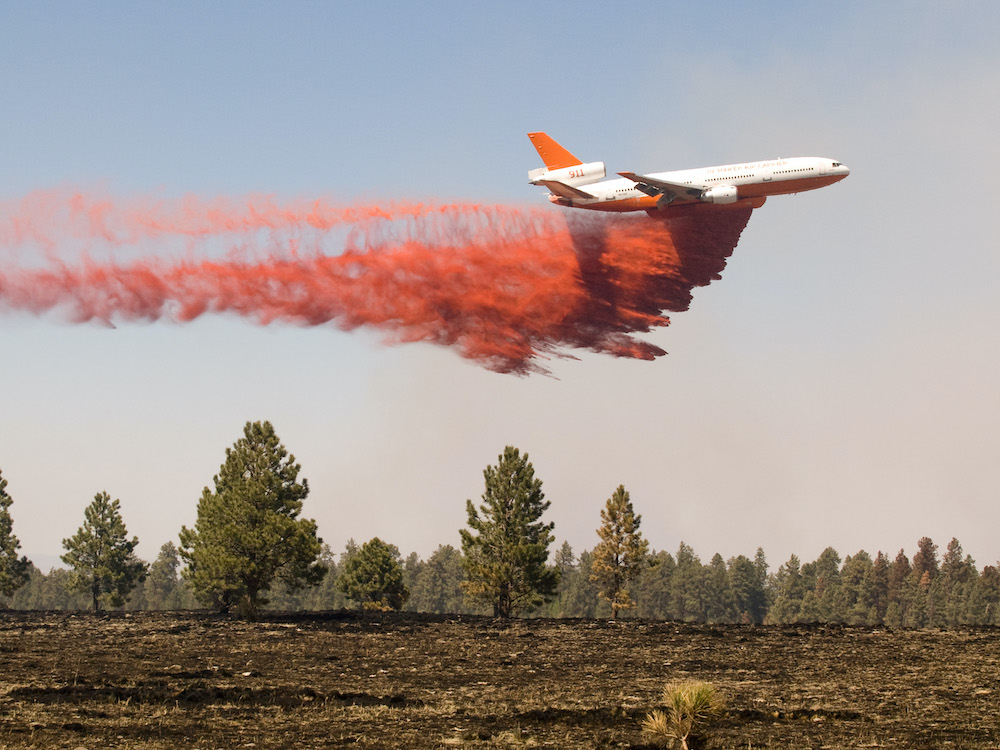
\includegraphics[scale=0.4]{images/dc10.jpg}
  \caption{A DC-10 airtanker, rated for 9,400 gallons, drops retardant above Greer, Arizona.}
\end{figure}

\begin{figure}[h]
  \centering
  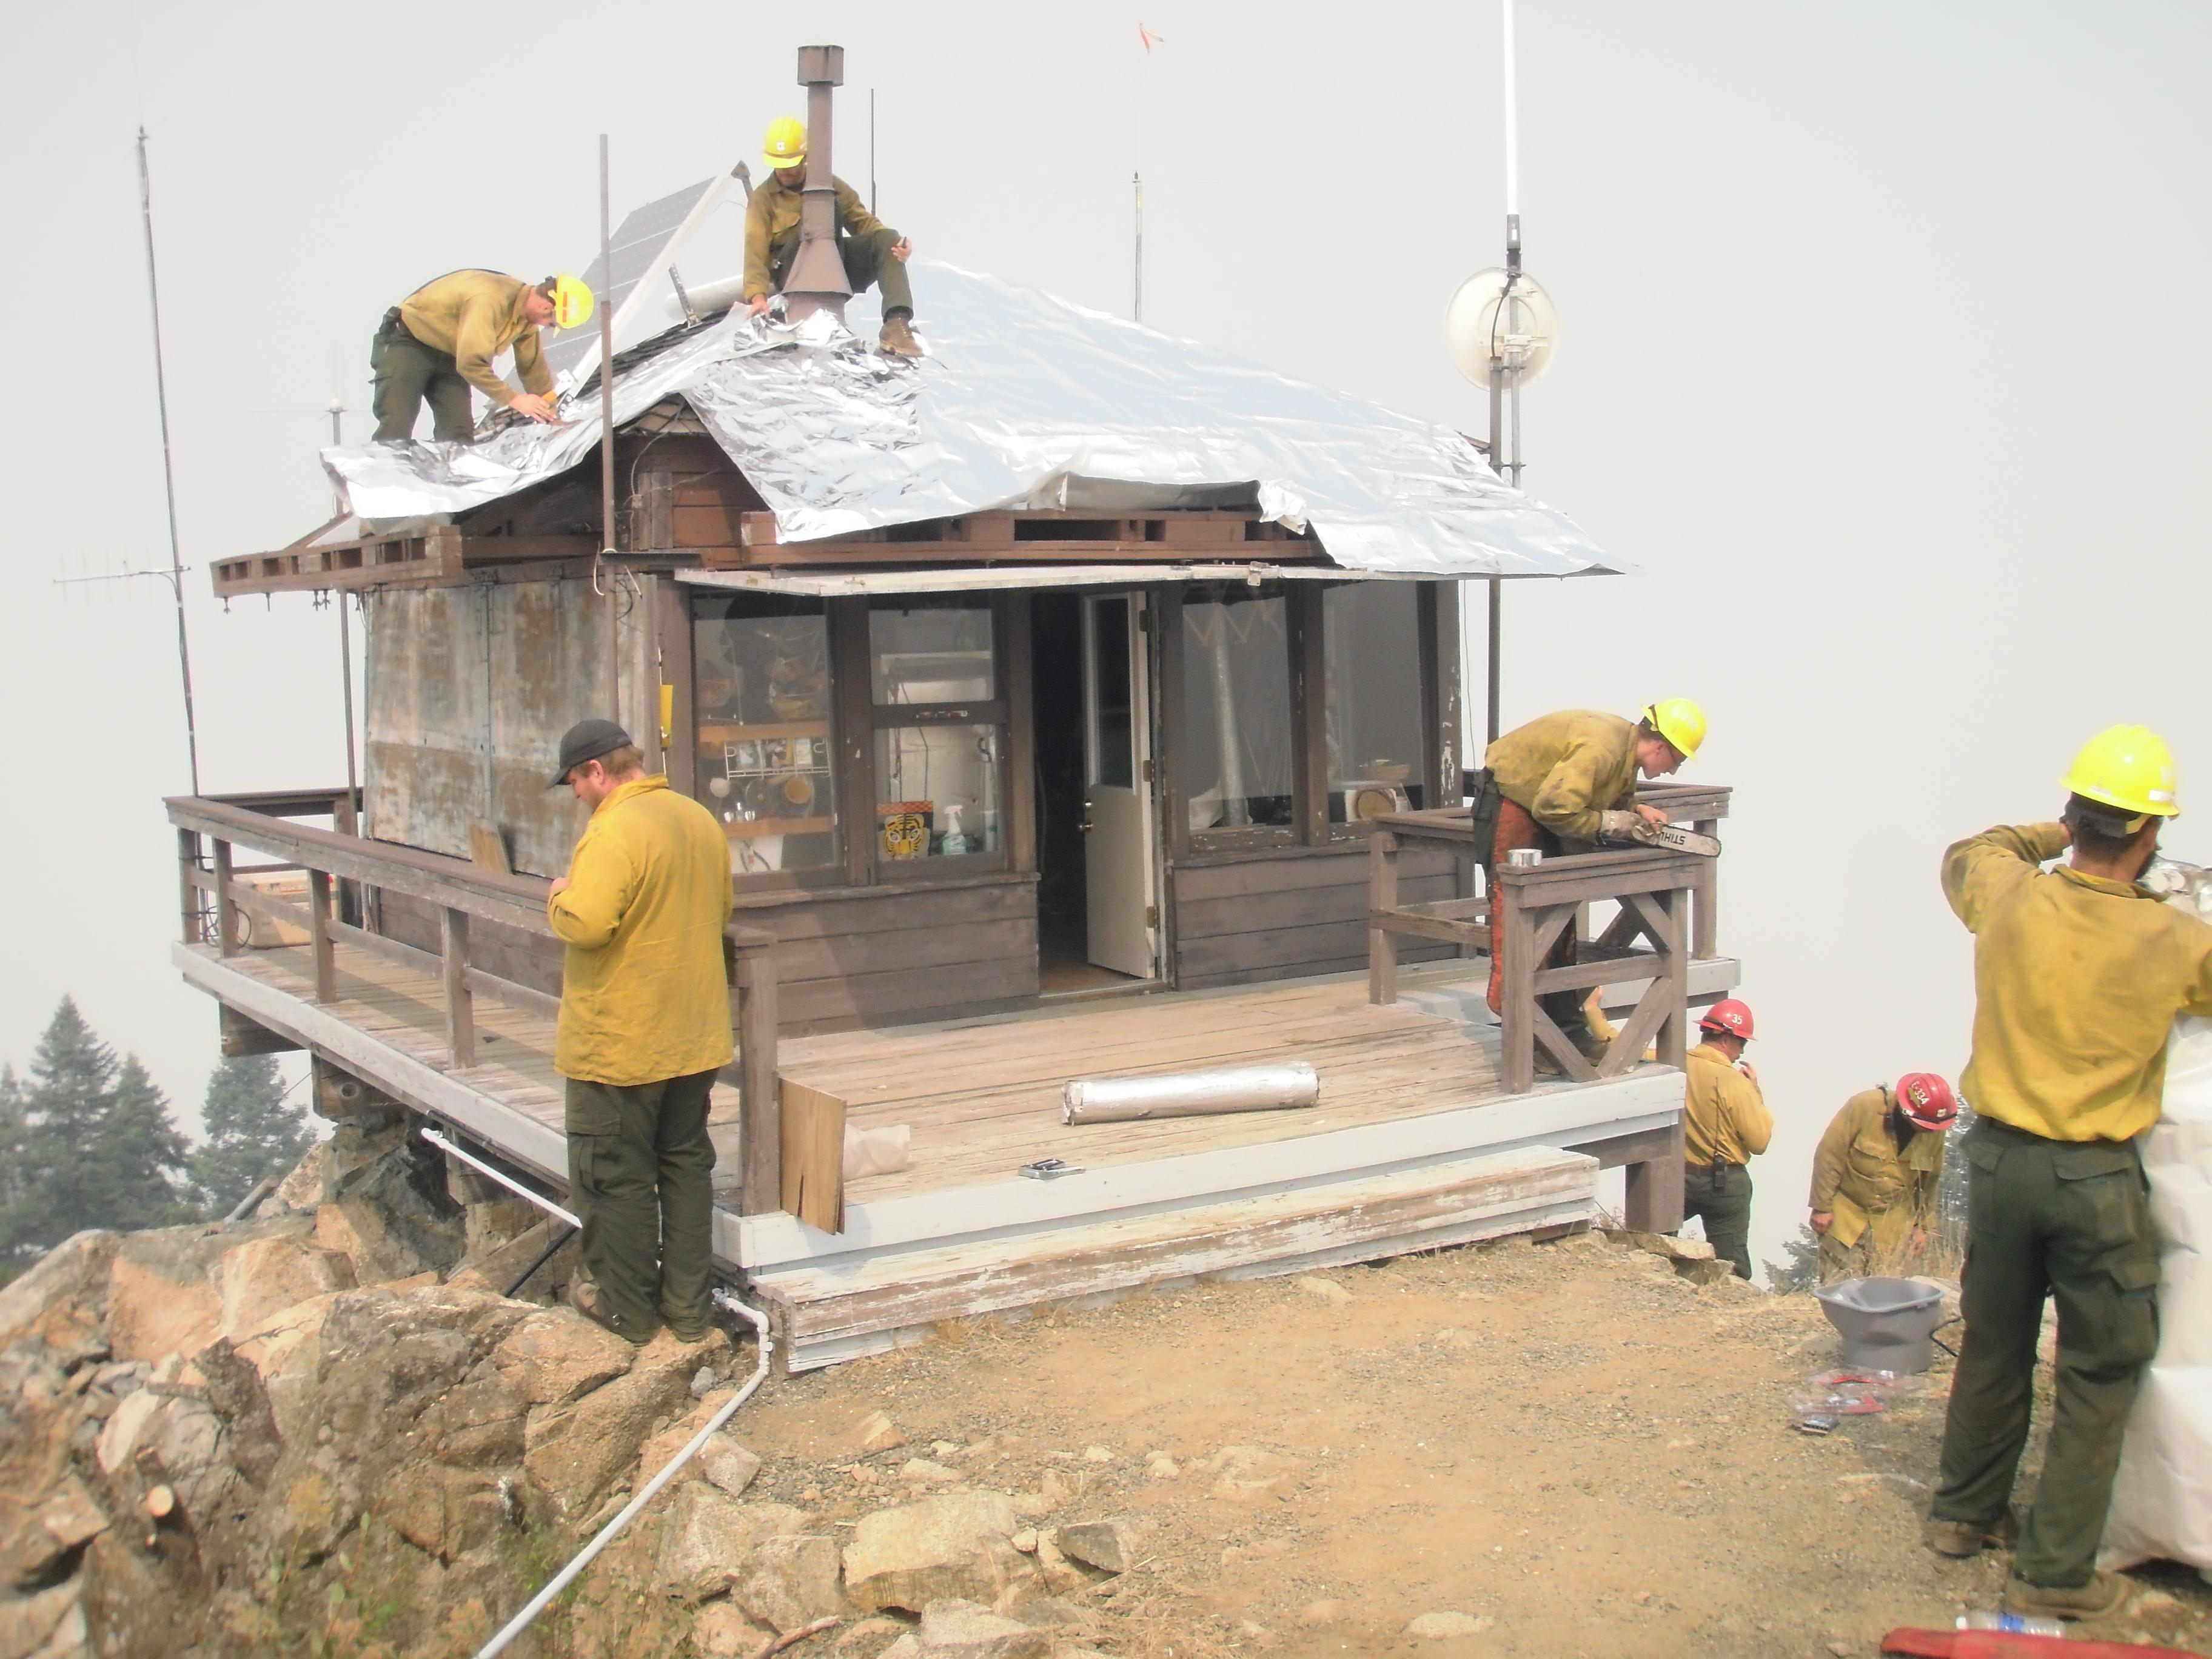
\includegraphics[scale=0.085]{images/ironside.jpg}
  \caption{The Ironside Mountain lookout station, destroyed in the 2021
    Monument fire, shown with protective foil on August
    $10^\textrm{th}$, 2015 during the 2015 River Complex fire. This
    particular fire burned 77,077 acres over 77 days.}
\end{figure}

\subsection{Communication Patterns in the Field}
\label{communication-in-practice}

Communication patterns in modern wildland firefighting are mostly
simple, even primitive in comparison to what laymen often expect.

In the examples below, we note a kind of ``geospatial locality of
reference'' that system designers should take into account. Generally
speaking, we expect that agents with a higher need to coordinate their
actions will tend to be located closer to each other, which in turn
correlates with an ability to communicate quickly and reliably. This
kind of principle motivates the sort of decentralized, ad-hoc networking
protocols considered in Section \ref{sec:networking}. It can also affect
the design of higher-level applications like the one in Section
\ref{sec:continuous-consistency}.

\paragraph{Communication on the ground}

In the field, communication between firefighters and other agents in
disaster response scenarios is often facilitated by handheld (analog)
radios, which are inherently limited in their battery life,\footnote{A
coordinator for NIFS reported that during peak demand, wildland
firefighters in the United States go through upwards of a combined
350,000 ``AA'' batteries in a day.} bandwidth, effective range, and
ability to work around environmental factors like foliage and smoke.

As an alternative to using a radio, it is common for wildland
firefighters in the field to communicate using the simplest of
technologies: shouting back and forth. Besides highlighting the fact
that sometimes simple things work, this is a clear manifestation of
geolocality of reference: firefighters mostly need to communicate when
they are working near each other, in some cases so nearby they can
communicate without network infrastructure.

Communicating over a long distance typically requires infrastructural
support, such as the use of cell towers and repeater
stations. Typically, disaster response environments have scarce
permanent infrastructure: perhaps a few repeaters mounted to a watch
tower for a wildland fire setting. Ad-hoc infrastructure, such as a
cell on wheels (COW) or cell on light truck (COLT), can sometimes be
deployed on an as-needed basis if the location allows for it. A common
issue is making sure that all equipment is properly configured, for
instance that all radios are listening on the correct frequencies,
particularly when different agencies and groups need to interoperate.

Use of centralized infrastructure comes at the cost of potential
widespread failure when the infrastructure fails. For example, in
California, the Ironside Mountain lookout/repeater station was destroyed
during the 2021 Monument Fire,\footnote{https://www.fire.ca.gov/incidents/2021/7/30/monument-fire/}
which burned approximately 184,142 acres over 88 days. The Ironside
Mountain station had strategic importance, being located on a tall
ridge. According to a video blog from a volunteer firefighter involved
in the incident (CITE), its loss prevented communication between
operators on different sides of the ridge, in networking parlance
creating a \emph{partition} that lasted until crews could ascend the
ridge to deploy a temporary station. This is exactly the kind of
scenario considered by Brewer's CAP theorem in Section
\ref{sec:background}.

\begin{quote}
  When {[}the Ironside Mountain lookout station{]} burned down the radio
  repeater went with it. And so communications were lost across the
  fire\ldots{} one side of the fire couldn't talk to the other side\ldots.
  So it was kind of a critical job to get that road cleared so that the
  radio crews could go back up there and set up a temporary radio tower.
\end{quote}

\paragraph{Vehicles on the ground}
Large numbers of ground vehicles are involved in wildfire
suppression. A large wildfire response can involve more than 50--100
firetrucks distributed over a large geographical area. Bulldozers and
similar vehicles are commonly used to control the landscape and
perimeter of the fire. An advantage of vehicles is that they can carry
heavier, which is to say better, communications equipment than a
human. For instance, a vehicle could be equipped with a satellite link
as well as a local wireless area network (WLAN) base station, serving
as a bridge between agents in the field and central coordinators
(e.g. incident commanders).

\paragraph{Communication in the air}

Wildland firefighting increasingly involves the use of helicopters and
fixed wing aircraft, but civil aviation has traditionally employed
simpler communication patterns than this use case demands. For instance,
aircraft equipped with Automatic Dependent Surveillance-Broadcast
(ADS-B) monitor their location using GPS and periodically broadcast this
information to air traffic controllers and nearby aircraft. This sort of
scheme has worked well in traditional applications, where pilots
typically only monitor the general locations of a few nearby aircraft.
The locality principle is exhibited here, too: aircraft have the highest
need to coordinate when they are physically close and therefore in range
of each other's ADS-B broadcasts.

In our setting, a large number or aircraft, easily a half dozen or
more, may need to operate in a small area, near complex terrain,
during adverse conditions, often at a low altitude.\footnote{Current
recommendations (WHOSE) call for VLATs to perform drops at 250
ft. above the tree canopy, while smaller aircraft may go lower.} In
other words, the demands are many and the margins for error are
small. This sort of use case requires more sophisticated coordination
schemes between airborne and ground-based elements than solutions like
ADS-B provide by themselves.

As aircraft generally have better line-of-site to ground crews than
ground crews have to each other, firefighters sometimes relay messages
to air-based units over radio, which in turn is relayed back down to
other ground units. The locality principle comes into play here too, but
this time in the reverse direction: this relay scheme allows knowledge
to travel farther, but the extended reach comes at the cost of
introducing delays and possible degradation of message quality, as in
the classic game of telephone.

In some cases, planes from the Civil Air Patrol\footnote{A civil
auxiliary of the U.S. Air Force. https://www.gocivilairpatrol.com/}
(CITE) have been equipped with radio repeaters and dispatched to
wildfires to provide service to ground-based units. In the future, this
sort of service could be provided, perhaps autonomously, by base
stations mounted to unmanned aerial vehicles (UAVs), which might perform
additional functions such as tracking the fire perimeter. More
generally, a future communication system should exploit every pass
messages between agents, even in the event of infrastructure failure, in
a transparent and decentralized fashion. For instance, firefighters may
use an ad-hoc network built from handheld devices, vehicle-mounted
devices, temporary structure, an devices attached to overhead aircraft.
In effect, this would be a high-tech modernization of the sort of
informal relay schemes operating today over traditional radio channels.

\subsection{Towards the Future}\label{towards-the-future}

\begin{itemize}
  \tightlist
\item
  CITE developed a prototype application for firefighters in the field.
\item
  Talk about other applications
\end{itemize}

Taking a broader view, agents in disaster response environments will
often be both producers and consumers of data, and this data will need
to processed for agents to make informed decisions. Our background
research indicated many different kinds of data that could be valuable
for responders. To give just a glimpse:

\begin{itemize}
  \tightlist
\item
  Free-form communication, especially recorded voice messages to be
  broadcast to many firefighters at once.
\item
  The exact or estimated location of firefighters, vehicles, victims,
  hazards, etc.
\item
  Medical information, perhaps collected from digital triage tags (CITE)
\item
  Data about current and predicted fire or weather patterns
\item
  Topographic information about the terrain, highlighting for instance
  the location of rivers and roads that could form a fire control line
\item
  Planned escape routes, safety zones, and landing zones
\item
  Availability and dispatching of resources, e.g.~ambulances,
  airtankers, or crews on standby
\end{itemize}

In a perfect environment, such information would be shared with all
necessary agents in whole and instantly. In reality, agents will be
presented with information that is sometimes incomplete, out of date, or
contradictory---all problems that are further exacerbated by an
unreliable network.

For instance, a central data fusion center may be used to detect and
alert responders to a fire that has accidentally moved beyond a control
line (known as \emph{slopover}). Such information would be of high
importance, and it would be worthwhile to expend network resources
conveying this information to the relevant parties. On the other hand, a
firefighter may not need the minute GPS position of every other
firefighter in the field: perhaps the exact location of teammates, and
the general location of other crews.

Warn firefighters when they are too far from an escape route or safety zone.

For developers, it is clear that this requires some coordination between
the application and the networking layers, as the latter must be given
enough information to make the most prudent use of limited resources.

\section{Introduction to Distributed Systems}
\label{sec:background}
In this section we attempt to summarize the main themes of distributed
systems theory and where this fits into the picture painted in Section
\ref{sec:disaster-response}. The primary reference we are following is
the excellent book by Kshemkalyani and Singhal
\cite{kshemkalyani_singhal_2008}, particularly chapters 1, 3, 6, and
12.

A distributed system, in the most general sense, is a collection of
independent entities that cooperate to solve a problem that cannot be
individually solved \cite{kshemkalyani_singhal_2008}. This memo is
concerned with distributed systems used by firefighters and other
disaster response agents. The components of our system could be
computers, smartphones, various types of sensors, or other kinds of
communication and networking equipment. These may be personal devices
carried by individuals, mounted to ground or air-based vehicles, or be
deployed as temporary or permanent infrastructure. The clients of
these devices could be civilians, firefighters, incident commanders,
or other agents involved in disaster response efforts. The devices
could also be autonomous. The kinds of tasks our system or its
components might handle include navigating safely in close proximity,
delivering resources to remote locations, suppressing fires, and
collecting, processing, and disseminating data about the environment.

\subsection{Message Passing and Logical Time}
\label{ssec:message-passing}

Singhal and Shivaratri \cite{10.5555/562065} offer the following
definition of a distributed computing system:

\begin{quote}
  ``A collection of computers that do not share common memory or a common
  physical clock, that communicate by message passing over a communication
  network, and where each computer has its own memory and runs its own
  operating system.''
\end{quote}
We shall consider a system consisting of a set \(\mathcal{P} =
\{P_i\}_{i\in I}\) of \emph{processes} executing on independent,
probably geographically dispersed computing and communication
devices. We consolidate the various kinds of devices under the generic
term \emph{nodes}. It is important to note that different kinds of
nodes can have different characteristics, such as capabilities and
intended uses, but for now we take a high-level view. A notable aspect
of what makes the system ``distributed'' is that the nodes must
communicate by message-passing, which must be facilitated by some kind
of network. This restriction is implied by absence of a common memory
(whereas processes running on the same machine can share information
by writing it to a common memory location).

A foundational assumption is that the network is unreliable. Section
\ref{sec:disaster-response} explained why this is certainly expected
in disaster scenarios. Delivering messages over the network is not
instantaneous---message packets must be sent over the air or through a
cable, and typically processed and forwarded by any number of
intermediate networking devices, and retransmitted in case of
unrecoverable errors during transit, all of which takes time. This
means that messages are passed with some unpredictable latency. In
this section, our main challenge is to provide ways for agents to
coordinate their actions despite the uncontrollable delays in
communication caused by the network and environment, which is to say
by the ``distributed'' aspect of the system.

\paragraph{Network Reliability}
In full generality, the latency involved in sending messages need not
even be finite, meaning the network may not deliver a packet at all,
i.e.~it may silently discard the packet without alerting the
sender. The same message may be also be delivered multiple times, and
different messages may arrive in any order. In the case of
\emph{Byzantine faults}\citationneeded, the network might even act
like a malicious adversary. In this section, being focused on
higher-level considerations, we shall assume that messages are
delivered exactly once, uncorrupted, but with an unpredictable
delay. Some, but not all, common so-called ``transport'' protocols
like TCP\citationneeded and LTP\citationneeded can provide this sort
of semi-reliable message delivery over a less reliable network. For
example, these protocols might tag outgoing messages with an sequence
of unique identifiers that allow the receiver to detect duplicates and
arrange messages in the ordered intended by the sender; commonly they
also add checksums used to verify message integrity, and transparently
handle retranmission when messages become corrupted. For now, one
could say we are working at a level of abstraction above the network
transport layer. (We shall take a closer look at these kinds of
low-level details in Section \ref{sec:networking}, where we relax our
assumptions about network reliability.) Note that reliability
mechanisms in transport-level protocols contribute to the latencies
involved in message passing, so they do not solve the problems under
consideration here, namely the difficulty of coordination when
messages are unpredictably delayed and when nodes do not have access
to sychronized clocks.

\subsubsection{FIFO and causal ordering}

Figures \ref{fig:message-latencies} and \ref{fig:message-latencies2}
show time diagrams for messages $\{m_i\}_{i=1}^N$ sent between three
processes $P_1$, $P_2$, and $P_3$. The $x$-axis of the diagram shows
the flow of physical time from left to right. Each process consists of
a worldline depicting the events occurring in that process. Each
message $m_i$ starts off as a message \emph{send} event
$m_i^\textrm{send}$ indicating the moment the message is sent over the
network by its originating process; its delivery generates a message
\emph{receive} event $m_i^\textrm{recv}$. The corresponding events are
connected by an arrow.  The subscripts on the messages only serve to
disambiguate them, but they are not part of the message contents and
have no semantic importance.

\begin{figure}[p]
  \centering \begin{pgfpicture}
\pgfpathrectangle{\pgfpointorigin}{\pgfqpoint{380.0000bp}{150.0000bp}}
\pgfusepath{use as bounding box}
\begin{pgfscope}
\pgfsetlinewidth{1.0000bp}
\definecolor{sc}{rgb}{0.0000,0.0000,0.0000}
\pgfsetstrokecolor{sc}
\pgfsetmiterjoin
\pgfsetbuttcap
\pgfpathqmoveto{70.0000bp}{75.0000bp}
\pgfpathqlineto{115.6430bp}{124.7924bp}
\pgfusepathqstroke
\end{pgfscope}
\begin{pgfscope}
\definecolor{fc}{rgb}{0.0000,0.0000,0.0000}
\pgfsetfillcolor{fc}
\pgfusepathqfill
\end{pgfscope}
\begin{pgfscope}
\definecolor{fc}{rgb}{0.0000,0.0000,0.0000}
\pgfsetfillcolor{fc}
\pgfusepathqfill
\end{pgfscope}
\begin{pgfscope}
\definecolor{fc}{rgb}{0.0000,0.0000,0.0000}
\pgfsetfillcolor{fc}
\pgfpathqmoveto{121.2895bp}{130.9522bp}
\pgfpathqlineto{112.3562bp}{125.9001bp}
\pgfpathqlineto{115.8207bp}{124.9862bp}
\pgfpathqlineto{117.0318bp}{121.6141bp}
\pgfpathqlineto{121.2895bp}{130.9522bp}
\pgfpathclose
\pgfusepathqfill
\end{pgfscope}
\begin{pgfscope}
\definecolor{fc}{rgb}{0.0000,0.0000,0.0000}
\pgfsetfillcolor{fc}
\pgfpathqmoveto{115.8207bp}{124.9862bp}
\pgfpathqlineto{115.6430bp}{124.7924bp}
\pgfpathqlineto{115.2745bp}{125.1303bp}
\pgfpathqlineto{115.8207bp}{124.9862bp}
\pgfpathqlineto{115.6430bp}{124.7924bp}
\pgfpathqlineto{116.0116bp}{124.4545bp}
\pgfpathqlineto{115.8207bp}{124.9862bp}
\pgfpathclose
\pgfusepathqfill
\end{pgfscope}
\begin{pgfscope}
\pgfsetlinewidth{1.0000bp}
\definecolor{sc}{rgb}{0.0000,0.0000,0.0000}
\pgfsetstrokecolor{sc}
\pgfsetmiterjoin
\pgfsetbuttcap
\pgfpathqmoveto{170.0000bp}{135.0000bp}
\pgfpathqlineto{215.6430bp}{85.2076bp}
\pgfusepathqstroke
\end{pgfscope}
\begin{pgfscope}
\definecolor{fc}{rgb}{0.0000,0.0000,0.0000}
\pgfsetfillcolor{fc}
\pgfusepathqfill
\end{pgfscope}
\begin{pgfscope}
\definecolor{fc}{rgb}{0.0000,0.0000,0.0000}
\pgfsetfillcolor{fc}
\pgfusepathqfill
\end{pgfscope}
\begin{pgfscope}
\definecolor{fc}{rgb}{0.0000,0.0000,0.0000}
\pgfsetfillcolor{fc}
\pgfpathqmoveto{221.2895bp}{79.0478bp}
\pgfpathqlineto{217.0318bp}{88.3859bp}
\pgfpathqlineto{215.8207bp}{85.0138bp}
\pgfpathqlineto{212.3562bp}{84.0999bp}
\pgfpathqlineto{221.2895bp}{79.0478bp}
\pgfpathclose
\pgfusepathqfill
\end{pgfscope}
\begin{pgfscope}
\definecolor{fc}{rgb}{0.0000,0.0000,0.0000}
\pgfsetfillcolor{fc}
\pgfpathqmoveto{215.8207bp}{85.0138bp}
\pgfpathqlineto{215.6430bp}{85.2076bp}
\pgfpathqlineto{216.0116bp}{85.5455bp}
\pgfpathqlineto{215.8207bp}{85.0138bp}
\pgfpathqlineto{215.6430bp}{85.2076bp}
\pgfpathqlineto{215.2745bp}{84.8697bp}
\pgfpathqlineto{215.8207bp}{85.0138bp}
\pgfpathclose
\pgfusepathqfill
\end{pgfscope}
\begin{pgfscope}
\pgfsetlinewidth{1.0000bp}
\definecolor{sc}{rgb}{0.0000,0.0000,0.0000}
\pgfsetstrokecolor{sc}
\pgfsetmiterjoin
\pgfsetbuttcap
\pgfpathqmoveto{140.0000bp}{15.0000bp}
\pgfpathqlineto{333.0496bp}{128.0046bp}
\pgfusepathqstroke
\end{pgfscope}
\begin{pgfscope}
\definecolor{fc}{rgb}{0.0000,0.0000,0.0000}
\pgfsetfillcolor{fc}
\pgfusepathqfill
\end{pgfscope}
\begin{pgfscope}
\definecolor{fc}{rgb}{0.0000,0.0000,0.0000}
\pgfsetfillcolor{fc}
\pgfusepathqfill
\end{pgfscope}
\begin{pgfscope}
\definecolor{fc}{rgb}{0.0000,0.0000,0.0000}
\pgfsetfillcolor{fc}
\pgfpathqmoveto{340.2610bp}{132.2260bp}
\pgfpathqlineto{330.2354bp}{130.0321bp}
\pgfpathqlineto{333.2764bp}{128.1374bp}
\pgfpathqlineto{333.4396bp}{124.5582bp}
\pgfpathqlineto{340.2610bp}{132.2260bp}
\pgfpathclose
\pgfusepathqfill
\end{pgfscope}
\begin{pgfscope}
\definecolor{fc}{rgb}{0.0000,0.0000,0.0000}
\pgfsetfillcolor{fc}
\pgfpathqmoveto{333.2764bp}{128.1374bp}
\pgfpathqlineto{333.0496bp}{128.0046bp}
\pgfpathqlineto{332.7970bp}{128.4361bp}
\pgfpathqlineto{333.2764bp}{128.1374bp}
\pgfpathqlineto{333.0496bp}{128.0046bp}
\pgfpathqlineto{333.3022bp}{127.5731bp}
\pgfpathqlineto{333.2764bp}{128.1374bp}
\pgfpathclose
\pgfusepathqfill
\end{pgfscope}
\begin{pgfscope}
\pgfsetlinewidth{1.0000bp}
\definecolor{sc}{rgb}{0.0000,0.0000,0.0000}
\pgfsetstrokecolor{sc}
\pgfsetmiterjoin
\pgfsetbuttcap
\pgfpathqmoveto{285.0000bp}{75.0000bp}
\pgfpathqlineto{339.8249bp}{24.3924bp}
\pgfusepathqstroke
\end{pgfscope}
\begin{pgfscope}
\definecolor{fc}{rgb}{0.0000,0.0000,0.0000}
\pgfsetfillcolor{fc}
\pgfusepathqfill
\end{pgfscope}
\begin{pgfscope}
\definecolor{fc}{rgb}{0.0000,0.0000,0.0000}
\pgfsetfillcolor{fc}
\pgfusepathqfill
\end{pgfscope}
\begin{pgfscope}
\definecolor{fc}{rgb}{0.0000,0.0000,0.0000}
\pgfsetfillcolor{fc}
\pgfpathqmoveto{345.9651bp}{18.7246bp}
\pgfpathqlineto{340.9441bp}{27.6753bp}
\pgfpathqlineto{340.0181bp}{24.2141bp}
\pgfpathqlineto{336.6419bp}{23.0146bp}
\pgfpathqlineto{345.9651bp}{18.7246bp}
\pgfpathclose
\pgfusepathqfill
\end{pgfscope}
\begin{pgfscope}
\definecolor{fc}{rgb}{0.0000,0.0000,0.0000}
\pgfsetfillcolor{fc}
\pgfpathqmoveto{340.0181bp}{24.2141bp}
\pgfpathqlineto{339.8249bp}{24.3924bp}
\pgfpathqlineto{340.1641bp}{24.7598bp}
\pgfpathqlineto{340.0181bp}{24.2141bp}
\pgfpathqlineto{339.8249bp}{24.3924bp}
\pgfpathqlineto{339.4858bp}{24.0250bp}
\pgfpathqlineto{340.0181bp}{24.2141bp}
\pgfpathclose
\pgfusepathqfill
\end{pgfscope}
\begin{pgfscope}
\pgfsetlinewidth{1.0000bp}
\definecolor{sc}{rgb}{0.0000,0.0000,0.0000}
\pgfsetstrokecolor{sc}
\pgfsetmiterjoin
\pgfsetbuttcap
\pgfpathqmoveto{80.0000bp}{135.0000bp}
\pgfpathqlineto{277.9772bp}{21.8702bp}
\pgfusepathqstroke
\end{pgfscope}
\begin{pgfscope}
\definecolor{fc}{rgb}{0.0000,0.0000,0.0000}
\pgfsetfillcolor{fc}
\pgfusepathqfill
\end{pgfscope}
\begin{pgfscope}
\definecolor{fc}{rgb}{0.0000,0.0000,0.0000}
\pgfsetfillcolor{fc}
\pgfusepathqfill
\end{pgfscope}
\begin{pgfscope}
\definecolor{fc}{rgb}{0.0000,0.0000,0.0000}
\pgfsetfillcolor{fc}
\pgfpathqmoveto{285.2323bp}{17.7244bp}
\pgfpathqlineto{278.3312bp}{25.3205bp}
\pgfpathqlineto{278.2054bp}{21.7398bp}
\pgfpathqlineto{275.1843bp}{19.8134bp}
\pgfpathqlineto{285.2323bp}{17.7244bp}
\pgfpathclose
\pgfusepathqfill
\end{pgfscope}
\begin{pgfscope}
\definecolor{fc}{rgb}{0.0000,0.0000,0.0000}
\pgfsetfillcolor{fc}
\pgfpathqmoveto{278.2054bp}{21.7398bp}
\pgfpathqlineto{277.9772bp}{21.8702bp}
\pgfpathqlineto{278.2252bp}{22.3043bp}
\pgfpathqlineto{278.2054bp}{21.7398bp}
\pgfpathqlineto{277.9772bp}{21.8702bp}
\pgfpathqlineto{277.7291bp}{21.4361bp}
\pgfpathqlineto{278.2054bp}{21.7398bp}
\pgfpathclose
\pgfusepathqfill
\end{pgfscope}
\begin{pgfscope}
\pgfsetlinewidth{1.0000bp}
\definecolor{sc}{rgb}{0.0000,0.0000,0.0000}
\pgfsetstrokecolor{sc}
\pgfsetmiterjoin
\pgfsetbuttcap
\pgfpathqmoveto{30.0000bp}{15.0000bp}
\pgfpathqlineto{374.5088bp}{15.0000bp}
\pgfusepathqstroke
\end{pgfscope}
\begin{pgfscope}
\definecolor{fc}{rgb}{0.0000,0.0000,0.0000}
\pgfsetfillcolor{fc}
\pgfusepathqfill
\end{pgfscope}
\begin{pgfscope}
\definecolor{fc}{rgb}{0.0000,0.0000,0.0000}
\pgfsetfillcolor{fc}
\pgfusepathqfill
\end{pgfscope}
\begin{pgfscope}
\definecolor{fc}{rgb}{0.0000,0.0000,0.0000}
\pgfsetfillcolor{fc}
\pgfpathqmoveto{380.0000bp}{15.0000bp}
\pgfpathqlineto{374.5088bp}{18.1703bp}
\pgfpathqlineto{374.5088bp}{11.8297bp}
\pgfpathqlineto{380.0000bp}{15.0000bp}
\pgfpathclose
\pgfusepathqfill
\end{pgfscope}
\begin{pgfscope}
\definecolor{fc}{rgb}{0.0000,0.0000,0.0000}
\pgfsetfillcolor{fc}
\pgfusepathqfill
\end{pgfscope}
\begin{pgfscope}
\definecolor{fc}{rgb}{0.0000,0.0000,0.0000}
\pgfsetfillcolor{fc}
\pgfsetfillopacity{0.0000}
\pgfpathqmoveto{30.0000bp}{5.0000bp}
\pgfpathqlineto{30.0000bp}{25.0000bp}
\pgfpathqlineto{0.0000bp}{25.0000bp}
\pgfpathqlineto{-0.0000bp}{5.0000bp}
\pgfpathqlineto{30.0000bp}{5.0000bp}
\pgfpathclose
\pgfusepathqfill
\end{pgfscope}
\begin{pgfscope}
\definecolor{fc}{rgb}{0.0000,0.0000,0.0000}
\pgfsetfillcolor{fc}
\pgftransformshift{\pgfqpoint{15.0000bp}{15.0000bp}}
\pgftransformscale{0.6250}
\pgftext[]{$P_3$}
\end{pgfscope}
\begin{pgfscope}
\definecolor{fc}{rgb}{1.0000,1.0000,1.0000}
\pgfsetfillcolor{fc}
\pgfpathqmoveto{300.0000bp}{0.0000bp}
\pgfpathqlineto{300.0000bp}{10.0000bp}
\pgfpathqlineto{280.0000bp}{10.0000bp}
\pgfpathqlineto{280.0000bp}{0.0000bp}
\pgfpathqlineto{300.0000bp}{0.0000bp}
\pgfpathclose
\pgfusepathqfill
\end{pgfscope}
\begin{pgfscope}
\definecolor{fc}{rgb}{0.0000,0.0000,0.0000}
\pgfsetfillcolor{fc}
\pgftransformshift{\pgfqpoint{290.0000bp}{5.0000bp}}
\pgftransformscale{0.6250}
\pgftext[]{$m_2^\textrm{recv}$}
\end{pgfscope}
\begin{pgfscope}
\definecolor{fc}{rgb}{0.0000,0.0000,0.0000}
\pgfsetfillcolor{fc}
\pgfpathqmoveto{293.0000bp}{15.0000bp}
\pgfpathqcurveto{293.0000bp}{16.6569bp}{291.6569bp}{18.0000bp}{290.0000bp}{18.0000bp}
\pgfpathqcurveto{288.3431bp}{18.0000bp}{287.0000bp}{16.6569bp}{287.0000bp}{15.0000bp}
\pgfpathqcurveto{287.0000bp}{13.3431bp}{288.3431bp}{12.0000bp}{290.0000bp}{12.0000bp}
\pgfpathqcurveto{291.6569bp}{12.0000bp}{293.0000bp}{13.3431bp}{293.0000bp}{15.0000bp}
\pgfpathclose
\pgfusepathqfill
\end{pgfscope}
\begin{pgfscope}
\definecolor{fc}{rgb}{1.0000,1.0000,1.0000}
\pgfsetfillcolor{fc}
\pgfpathqmoveto{360.0000bp}{0.0000bp}
\pgfpathqlineto{360.0000bp}{10.0000bp}
\pgfpathqlineto{340.0000bp}{10.0000bp}
\pgfpathqlineto{340.0000bp}{0.0000bp}
\pgfpathqlineto{360.0000bp}{0.0000bp}
\pgfpathclose
\pgfusepathqfill
\end{pgfscope}
\begin{pgfscope}
\definecolor{fc}{rgb}{0.0000,0.0000,0.0000}
\pgfsetfillcolor{fc}
\pgftransformshift{\pgfqpoint{350.0000bp}{5.0000bp}}
\pgftransformscale{0.6250}
\pgftext[]{$m_5^\textrm{recv}$}
\end{pgfscope}
\begin{pgfscope}
\definecolor{fc}{rgb}{0.0000,0.0000,0.0000}
\pgfsetfillcolor{fc}
\pgfpathqmoveto{353.0000bp}{15.0000bp}
\pgfpathqcurveto{353.0000bp}{16.6569bp}{351.6569bp}{18.0000bp}{350.0000bp}{18.0000bp}
\pgfpathqcurveto{348.3431bp}{18.0000bp}{347.0000bp}{16.6569bp}{347.0000bp}{15.0000bp}
\pgfpathqcurveto{347.0000bp}{13.3431bp}{348.3431bp}{12.0000bp}{350.0000bp}{12.0000bp}
\pgfpathqcurveto{351.6569bp}{12.0000bp}{353.0000bp}{13.3431bp}{353.0000bp}{15.0000bp}
\pgfpathclose
\pgfusepathqfill
\end{pgfscope}
\begin{pgfscope}
\definecolor{fc}{rgb}{1.0000,1.0000,1.0000}
\pgfsetfillcolor{fc}
\pgfpathqmoveto{150.0000bp}{0.0000bp}
\pgfpathqlineto{150.0000bp}{10.0000bp}
\pgfpathqlineto{130.0000bp}{10.0000bp}
\pgfpathqlineto{130.0000bp}{0.0000bp}
\pgfpathqlineto{150.0000bp}{0.0000bp}
\pgfpathclose
\pgfusepathqfill
\end{pgfscope}
\begin{pgfscope}
\definecolor{fc}{rgb}{0.0000,0.0000,0.0000}
\pgfsetfillcolor{fc}
\pgftransformshift{\pgfqpoint{140.0000bp}{5.0000bp}}
\pgftransformscale{0.6250}
\pgftext[]{$m_3^\textrm{send}$}
\end{pgfscope}
\begin{pgfscope}
\definecolor{fc}{rgb}{0.0000,0.0000,0.0000}
\pgfsetfillcolor{fc}
\pgfpathqmoveto{143.0000bp}{15.0000bp}
\pgfpathqcurveto{143.0000bp}{16.6569bp}{141.6569bp}{18.0000bp}{140.0000bp}{18.0000bp}
\pgfpathqcurveto{138.3431bp}{18.0000bp}{137.0000bp}{16.6569bp}{137.0000bp}{15.0000bp}
\pgfpathqcurveto{137.0000bp}{13.3431bp}{138.3431bp}{12.0000bp}{140.0000bp}{12.0000bp}
\pgfpathqcurveto{141.6569bp}{12.0000bp}{143.0000bp}{13.3431bp}{143.0000bp}{15.0000bp}
\pgfpathclose
\pgfusepathqfill
\end{pgfscope}
\begin{pgfscope}
\pgfsetlinewidth{1.0000bp}
\definecolor{sc}{rgb}{0.0000,0.0000,0.0000}
\pgfsetstrokecolor{sc}
\pgfsetmiterjoin
\pgfsetbuttcap
\pgfpathqmoveto{30.0000bp}{75.0000bp}
\pgfpathqlineto{374.5088bp}{75.0000bp}
\pgfusepathqstroke
\end{pgfscope}
\begin{pgfscope}
\definecolor{fc}{rgb}{0.0000,0.0000,0.0000}
\pgfsetfillcolor{fc}
\pgfusepathqfill
\end{pgfscope}
\begin{pgfscope}
\definecolor{fc}{rgb}{0.0000,0.0000,0.0000}
\pgfsetfillcolor{fc}
\pgfusepathqfill
\end{pgfscope}
\begin{pgfscope}
\definecolor{fc}{rgb}{0.0000,0.0000,0.0000}
\pgfsetfillcolor{fc}
\pgfpathqmoveto{380.0000bp}{75.0000bp}
\pgfpathqlineto{374.5088bp}{78.1703bp}
\pgfpathqlineto{374.5088bp}{71.8297bp}
\pgfpathqlineto{380.0000bp}{75.0000bp}
\pgfpathclose
\pgfusepathqfill
\end{pgfscope}
\begin{pgfscope}
\definecolor{fc}{rgb}{0.0000,0.0000,0.0000}
\pgfsetfillcolor{fc}
\pgfusepathqfill
\end{pgfscope}
\begin{pgfscope}
\definecolor{fc}{rgb}{0.0000,0.0000,0.0000}
\pgfsetfillcolor{fc}
\pgfsetfillopacity{0.0000}
\pgfpathqmoveto{30.0000bp}{65.0000bp}
\pgfpathqlineto{30.0000bp}{85.0000bp}
\pgfpathqlineto{0.0000bp}{85.0000bp}
\pgfpathqlineto{-0.0000bp}{65.0000bp}
\pgfpathqlineto{30.0000bp}{65.0000bp}
\pgfpathclose
\pgfusepathqfill
\end{pgfscope}
\begin{pgfscope}
\definecolor{fc}{rgb}{0.0000,0.0000,0.0000}
\pgfsetfillcolor{fc}
\pgftransformshift{\pgfqpoint{15.0000bp}{75.0000bp}}
\pgftransformscale{0.6250}
\pgftext[]{$P_2$}
\end{pgfscope}
\begin{pgfscope}
\definecolor{fc}{rgb}{1.0000,1.0000,1.0000}
\pgfsetfillcolor{fc}
\pgfpathqmoveto{241.0000bp}{80.0000bp}
\pgfpathqlineto{241.0000bp}{90.0000bp}
\pgfpathqlineto{221.0000bp}{90.0000bp}
\pgfpathqlineto{221.0000bp}{80.0000bp}
\pgfpathqlineto{241.0000bp}{80.0000bp}
\pgfpathclose
\pgfusepathqfill
\end{pgfscope}
\begin{pgfscope}
\definecolor{fc}{rgb}{0.0000,0.0000,0.0000}
\pgfsetfillcolor{fc}
\pgftransformshift{\pgfqpoint{231.0000bp}{85.0000bp}}
\pgftransformscale{0.6250}
\pgftext[]{$m_4^\textrm{recv}$}
\end{pgfscope}
\begin{pgfscope}
\definecolor{fc}{rgb}{0.0000,0.0000,0.0000}
\pgfsetfillcolor{fc}
\pgfpathqmoveto{228.0000bp}{75.0000bp}
\pgfpathqcurveto{228.0000bp}{76.6569bp}{226.6569bp}{78.0000bp}{225.0000bp}{78.0000bp}
\pgfpathqcurveto{223.3431bp}{78.0000bp}{222.0000bp}{76.6569bp}{222.0000bp}{75.0000bp}
\pgfpathqcurveto{222.0000bp}{73.3431bp}{223.3431bp}{72.0000bp}{225.0000bp}{72.0000bp}
\pgfpathqcurveto{226.6569bp}{72.0000bp}{228.0000bp}{73.3431bp}{228.0000bp}{75.0000bp}
\pgfpathclose
\pgfusepathqfill
\end{pgfscope}
\begin{pgfscope}
\definecolor{fc}{rgb}{1.0000,1.0000,1.0000}
\pgfsetfillcolor{fc}
\pgfpathqmoveto{300.0000bp}{80.0000bp}
\pgfpathqlineto{300.0000bp}{90.0000bp}
\pgfpathqlineto{280.0000bp}{90.0000bp}
\pgfpathqlineto{280.0000bp}{80.0000bp}
\pgfpathqlineto{300.0000bp}{80.0000bp}
\pgfpathclose
\pgfusepathqfill
\end{pgfscope}
\begin{pgfscope}
\definecolor{fc}{rgb}{0.0000,0.0000,0.0000}
\pgfsetfillcolor{fc}
\pgftransformshift{\pgfqpoint{290.0000bp}{85.0000bp}}
\pgftransformscale{0.6250}
\pgftext[]{$m_5^\textrm{send}$}
\end{pgfscope}
\begin{pgfscope}
\definecolor{fc}{rgb}{0.0000,0.0000,0.0000}
\pgfsetfillcolor{fc}
\pgfpathqmoveto{288.0000bp}{75.0000bp}
\pgfpathqcurveto{288.0000bp}{76.6569bp}{286.6569bp}{78.0000bp}{285.0000bp}{78.0000bp}
\pgfpathqcurveto{283.3431bp}{78.0000bp}{282.0000bp}{76.6569bp}{282.0000bp}{75.0000bp}
\pgfpathqcurveto{282.0000bp}{73.3431bp}{283.3431bp}{72.0000bp}{285.0000bp}{72.0000bp}
\pgfpathqcurveto{286.6569bp}{72.0000bp}{288.0000bp}{73.3431bp}{288.0000bp}{75.0000bp}
\pgfpathclose
\pgfusepathqfill
\end{pgfscope}
\begin{pgfscope}
\definecolor{fc}{rgb}{1.0000,1.0000,1.0000}
\pgfsetfillcolor{fc}
\pgfpathqmoveto{80.0000bp}{60.0000bp}
\pgfpathqlineto{80.0000bp}{70.0000bp}
\pgfpathqlineto{60.0000bp}{70.0000bp}
\pgfpathqlineto{60.0000bp}{60.0000bp}
\pgfpathqlineto{80.0000bp}{60.0000bp}
\pgfpathclose
\pgfusepathqfill
\end{pgfscope}
\begin{pgfscope}
\definecolor{fc}{rgb}{0.0000,0.0000,0.0000}
\pgfsetfillcolor{fc}
\pgftransformshift{\pgfqpoint{70.0000bp}{65.0000bp}}
\pgftransformscale{0.6250}
\pgftext[]{$m_1^\textrm{send}$}
\end{pgfscope}
\begin{pgfscope}
\definecolor{fc}{rgb}{0.0000,0.0000,0.0000}
\pgfsetfillcolor{fc}
\pgfpathqmoveto{73.0000bp}{75.0000bp}
\pgfpathqcurveto{73.0000bp}{76.6569bp}{71.6569bp}{78.0000bp}{70.0000bp}{78.0000bp}
\pgfpathqcurveto{68.3431bp}{78.0000bp}{67.0000bp}{76.6569bp}{67.0000bp}{75.0000bp}
\pgfpathqcurveto{67.0000bp}{73.3431bp}{68.3431bp}{72.0000bp}{70.0000bp}{72.0000bp}
\pgfpathqcurveto{71.6569bp}{72.0000bp}{73.0000bp}{73.3431bp}{73.0000bp}{75.0000bp}
\pgfpathclose
\pgfusepathqfill
\end{pgfscope}
\begin{pgfscope}
\pgfsetlinewidth{1.0000bp}
\definecolor{sc}{rgb}{0.0000,0.0000,0.0000}
\pgfsetstrokecolor{sc}
\pgfsetmiterjoin
\pgfsetbuttcap
\pgfpathqmoveto{30.0000bp}{135.0000bp}
\pgfpathqlineto{374.5088bp}{135.0000bp}
\pgfusepathqstroke
\end{pgfscope}
\begin{pgfscope}
\definecolor{fc}{rgb}{0.0000,0.0000,0.0000}
\pgfsetfillcolor{fc}
\pgfusepathqfill
\end{pgfscope}
\begin{pgfscope}
\definecolor{fc}{rgb}{0.0000,0.0000,0.0000}
\pgfsetfillcolor{fc}
\pgfusepathqfill
\end{pgfscope}
\begin{pgfscope}
\definecolor{fc}{rgb}{0.0000,0.0000,0.0000}
\pgfsetfillcolor{fc}
\pgfpathqmoveto{380.0000bp}{135.0000bp}
\pgfpathqlineto{374.5088bp}{138.1703bp}
\pgfpathqlineto{374.5088bp}{131.8297bp}
\pgfpathqlineto{380.0000bp}{135.0000bp}
\pgfpathclose
\pgfusepathqfill
\end{pgfscope}
\begin{pgfscope}
\definecolor{fc}{rgb}{0.0000,0.0000,0.0000}
\pgfsetfillcolor{fc}
\pgfusepathqfill
\end{pgfscope}
\begin{pgfscope}
\definecolor{fc}{rgb}{0.0000,0.0000,0.0000}
\pgfsetfillcolor{fc}
\pgfsetfillopacity{0.0000}
\pgfpathqmoveto{30.0000bp}{125.0000bp}
\pgfpathqlineto{30.0000bp}{145.0000bp}
\pgfpathqlineto{0.0000bp}{145.0000bp}
\pgfpathqlineto{-0.0000bp}{125.0000bp}
\pgfpathqlineto{30.0000bp}{125.0000bp}
\pgfpathclose
\pgfusepathqfill
\end{pgfscope}
\begin{pgfscope}
\definecolor{fc}{rgb}{0.0000,0.0000,0.0000}
\pgfsetfillcolor{fc}
\pgftransformshift{\pgfqpoint{15.0000bp}{135.0000bp}}
\pgftransformscale{0.6250}
\pgftext[]{$P_1$}
\end{pgfscope}
\begin{pgfscope}
\definecolor{fc}{rgb}{1.0000,1.0000,1.0000}
\pgfsetfillcolor{fc}
\pgfpathqmoveto{355.0000bp}{140.0000bp}
\pgfpathqlineto{355.0000bp}{150.0000bp}
\pgfpathqlineto{335.0000bp}{150.0000bp}
\pgfpathqlineto{335.0000bp}{140.0000bp}
\pgfpathqlineto{355.0000bp}{140.0000bp}
\pgfpathclose
\pgfusepathqfill
\end{pgfscope}
\begin{pgfscope}
\definecolor{fc}{rgb}{0.0000,0.0000,0.0000}
\pgfsetfillcolor{fc}
\pgftransformshift{\pgfqpoint{345.0000bp}{145.0000bp}}
\pgftransformscale{0.6250}
\pgftext[]{$m_3^\textrm{recv}$}
\end{pgfscope}
\begin{pgfscope}
\definecolor{fc}{rgb}{0.0000,0.0000,0.0000}
\pgfsetfillcolor{fc}
\pgfpathqmoveto{348.0000bp}{135.0000bp}
\pgfpathqcurveto{348.0000bp}{136.6569bp}{346.6569bp}{138.0000bp}{345.0000bp}{138.0000bp}
\pgfpathqcurveto{343.3431bp}{138.0000bp}{342.0000bp}{136.6569bp}{342.0000bp}{135.0000bp}
\pgfpathqcurveto{342.0000bp}{133.3431bp}{343.3431bp}{132.0000bp}{345.0000bp}{132.0000bp}
\pgfpathqcurveto{346.6569bp}{132.0000bp}{348.0000bp}{133.3431bp}{348.0000bp}{135.0000bp}
\pgfpathclose
\pgfusepathqfill
\end{pgfscope}
\begin{pgfscope}
\definecolor{fc}{rgb}{1.0000,1.0000,1.0000}
\pgfsetfillcolor{fc}
\pgfpathqmoveto{180.0000bp}{140.0000bp}
\pgfpathqlineto{180.0000bp}{150.0000bp}
\pgfpathqlineto{160.0000bp}{150.0000bp}
\pgfpathqlineto{160.0000bp}{140.0000bp}
\pgfpathqlineto{180.0000bp}{140.0000bp}
\pgfpathclose
\pgfusepathqfill
\end{pgfscope}
\begin{pgfscope}
\definecolor{fc}{rgb}{0.0000,0.0000,0.0000}
\pgfsetfillcolor{fc}
\pgftransformshift{\pgfqpoint{170.0000bp}{145.0000bp}}
\pgftransformscale{0.6250}
\pgftext[]{$m_4^\textrm{send}$}
\end{pgfscope}
\begin{pgfscope}
\definecolor{fc}{rgb}{0.0000,0.0000,0.0000}
\pgfsetfillcolor{fc}
\pgfpathqmoveto{173.0000bp}{135.0000bp}
\pgfpathqcurveto{173.0000bp}{136.6569bp}{171.6569bp}{138.0000bp}{170.0000bp}{138.0000bp}
\pgfpathqcurveto{168.3431bp}{138.0000bp}{167.0000bp}{136.6569bp}{167.0000bp}{135.0000bp}
\pgfpathqcurveto{167.0000bp}{133.3431bp}{168.3431bp}{132.0000bp}{170.0000bp}{132.0000bp}
\pgfpathqcurveto{171.6569bp}{132.0000bp}{173.0000bp}{133.3431bp}{173.0000bp}{135.0000bp}
\pgfpathclose
\pgfusepathqfill
\end{pgfscope}
\begin{pgfscope}
\definecolor{fc}{rgb}{1.0000,1.0000,1.0000}
\pgfsetfillcolor{fc}
\pgfpathqmoveto{135.0000bp}{140.0000bp}
\pgfpathqlineto{135.0000bp}{150.0000bp}
\pgfpathqlineto{115.0000bp}{150.0000bp}
\pgfpathqlineto{115.0000bp}{140.0000bp}
\pgfpathqlineto{135.0000bp}{140.0000bp}
\pgfpathclose
\pgfusepathqfill
\end{pgfscope}
\begin{pgfscope}
\definecolor{fc}{rgb}{0.0000,0.0000,0.0000}
\pgfsetfillcolor{fc}
\pgftransformshift{\pgfqpoint{125.0000bp}{145.0000bp}}
\pgftransformscale{0.6250}
\pgftext[]{$m_1^\textrm{recv}$}
\end{pgfscope}
\begin{pgfscope}
\definecolor{fc}{rgb}{0.0000,0.0000,0.0000}
\pgfsetfillcolor{fc}
\pgfpathqmoveto{128.0000bp}{135.0000bp}
\pgfpathqcurveto{128.0000bp}{136.6569bp}{126.6569bp}{138.0000bp}{125.0000bp}{138.0000bp}
\pgfpathqcurveto{123.3431bp}{138.0000bp}{122.0000bp}{136.6569bp}{122.0000bp}{135.0000bp}
\pgfpathqcurveto{122.0000bp}{133.3431bp}{123.3431bp}{132.0000bp}{125.0000bp}{132.0000bp}
\pgfpathqcurveto{126.6569bp}{132.0000bp}{128.0000bp}{133.3431bp}{128.0000bp}{135.0000bp}
\pgfpathclose
\pgfusepathqfill
\end{pgfscope}
\begin{pgfscope}
\definecolor{fc}{rgb}{1.0000,1.0000,1.0000}
\pgfsetfillcolor{fc}
\pgfpathqmoveto{90.0000bp}{140.0000bp}
\pgfpathqlineto{90.0000bp}{150.0000bp}
\pgfpathqlineto{70.0000bp}{150.0000bp}
\pgfpathqlineto{70.0000bp}{140.0000bp}
\pgfpathqlineto{90.0000bp}{140.0000bp}
\pgfpathclose
\pgfusepathqfill
\end{pgfscope}
\begin{pgfscope}
\definecolor{fc}{rgb}{0.0000,0.0000,0.0000}
\pgfsetfillcolor{fc}
\pgftransformshift{\pgfqpoint{80.0000bp}{145.0000bp}}
\pgftransformscale{0.6250}
\pgftext[]{$m_2^\textrm{send}$}
\end{pgfscope}
\begin{pgfscope}
\definecolor{fc}{rgb}{0.0000,0.0000,0.0000}
\pgfsetfillcolor{fc}
\pgfpathqmoveto{83.0000bp}{135.0000bp}
\pgfpathqcurveto{83.0000bp}{136.6569bp}{81.6569bp}{138.0000bp}{80.0000bp}{138.0000bp}
\pgfpathqcurveto{78.3431bp}{138.0000bp}{77.0000bp}{136.6569bp}{77.0000bp}{135.0000bp}
\pgfpathqcurveto{77.0000bp}{133.3431bp}{78.3431bp}{132.0000bp}{80.0000bp}{132.0000bp}
\pgfpathqcurveto{81.6569bp}{132.0000bp}{83.0000bp}{133.3431bp}{83.0000bp}{135.0000bp}
\pgfpathclose
\pgfusepathqfill
\end{pgfscope}
\end{pgfpicture}

  \caption{Time diagram depicting latencies in message-passing}
  \label{fig:message-latencies}
\end{figure}

\begin{figure}[p]
  \centering \begin{pgfpicture}
\pgfpathrectangle{\pgfpointorigin}{\pgfqpoint{418.0000bp}{165.0000bp}}
\pgfusepath{use as bounding box}
\begin{pgfscope}
\pgfsetlinewidth{1.0000bp}
\definecolor{sc}{rgb}{0.0000,0.0000,0.0000}
\pgfsetstrokecolor{sc}
\pgfsetmiterjoin
\pgfsetbuttcap
\pgfpathqmoveto{53.0000bp}{21.5000bp}
\pgfpathqlineto{328.9253bp}{135.6760bp}
\pgfusepathqstroke
\end{pgfscope}
\begin{pgfscope}
\definecolor{fc}{rgb}{0.0000,0.0000,0.0000}
\pgfsetfillcolor{fc}
\pgfusepathqfill
\end{pgfscope}
\begin{pgfscope}
\definecolor{fc}{rgb}{0.0000,0.0000,0.0000}
\pgfsetfillcolor{fc}
\pgfusepathqfill
\end{pgfscope}
\begin{pgfscope}
\definecolor{fc}{rgb}{0.0000,0.0000,0.0000}
\pgfsetfillcolor{fc}
\pgfpathqmoveto{337.4187bp}{139.1905bp}
\pgfpathqlineto{326.1308bp}{138.3062bp}
\pgfpathqlineto{329.1682bp}{135.7765bp}
\pgfpathqlineto{328.8063bp}{131.8402bp}
\pgfpathqlineto{337.4187bp}{139.1905bp}
\pgfpathclose
\pgfusepathqfill
\end{pgfscope}
\begin{pgfscope}
\definecolor{fc}{rgb}{0.0000,0.0000,0.0000}
\pgfsetfillcolor{fc}
\pgfpathqmoveto{329.1682bp}{135.7765bp}
\pgfpathqlineto{328.9253bp}{135.6760bp}
\pgfpathqlineto{328.7342bp}{136.1380bp}
\pgfpathqlineto{329.1682bp}{135.7765bp}
\pgfpathqlineto{328.9253bp}{135.6760bp}
\pgfpathqlineto{329.1165bp}{135.2140bp}
\pgfpathqlineto{329.1682bp}{135.7765bp}
\pgfpathclose
\pgfusepathqfill
\end{pgfscope}
\begin{pgfscope}
\pgfsetlinewidth{1.0000bp}
\definecolor{sc}{rgb}{0.0000,0.0000,0.0000}
\pgfsetstrokecolor{sc}
\pgfsetmiterjoin
\pgfsetbuttcap
\pgfpathqmoveto{73.0000bp}{141.5000bp}
\pgfpathqlineto{88.1832bp}{95.9504bp}
\pgfusepathqstroke
\end{pgfscope}
\begin{pgfscope}
\definecolor{fc}{rgb}{0.0000,0.0000,0.0000}
\pgfsetfillcolor{fc}
\pgfusepathqfill
\end{pgfscope}
\begin{pgfscope}
\definecolor{fc}{rgb}{0.0000,0.0000,0.0000}
\pgfsetfillcolor{fc}
\pgfusepathqfill
\end{pgfscope}
\begin{pgfscope}
\definecolor{fc}{rgb}{0.0000,0.0000,0.0000}
\pgfsetfillcolor{fc}
\pgfpathqmoveto{91.0899bp}{87.2303bp}
\pgfpathqlineto{91.0039bp}{98.5525bp}
\pgfpathqlineto{88.2663bp}{95.7010bp}
\pgfpathqlineto{84.3654bp}{96.3396bp}
\pgfpathqlineto{91.0899bp}{87.2303bp}
\pgfpathclose
\pgfusepathqfill
\end{pgfscope}
\begin{pgfscope}
\definecolor{fc}{rgb}{0.0000,0.0000,0.0000}
\pgfsetfillcolor{fc}
\pgfpathqmoveto{88.2663bp}{95.7010bp}
\pgfpathqlineto{88.1832bp}{95.9504bp}
\pgfpathqlineto{88.6575bp}{96.1085bp}
\pgfpathqlineto{88.2663bp}{95.7010bp}
\pgfpathqlineto{88.1832bp}{95.9504bp}
\pgfpathqlineto{87.7089bp}{95.7923bp}
\pgfpathqlineto{88.2663bp}{95.7010bp}
\pgfpathclose
\pgfusepathqfill
\end{pgfscope}
\begin{pgfscope}
\pgfsetlinewidth{1.0000bp}
\definecolor{sc}{rgb}{0.0000,0.0000,0.0000}
\pgfsetstrokecolor{sc}
\pgfsetmiterjoin
\pgfsetbuttcap
\pgfpathqmoveto{113.0000bp}{81.5000bp}
\pgfpathqlineto{128.1832bp}{127.0496bp}
\pgfusepathqstroke
\end{pgfscope}
\begin{pgfscope}
\definecolor{fc}{rgb}{0.0000,0.0000,0.0000}
\pgfsetfillcolor{fc}
\pgfusepathqfill
\end{pgfscope}
\begin{pgfscope}
\definecolor{fc}{rgb}{0.0000,0.0000,0.0000}
\pgfsetfillcolor{fc}
\pgfusepathqfill
\end{pgfscope}
\begin{pgfscope}
\definecolor{fc}{rgb}{0.0000,0.0000,0.0000}
\pgfsetfillcolor{fc}
\pgfpathqmoveto{131.0899bp}{135.7697bp}
\pgfpathqlineto{124.3654bp}{126.6604bp}
\pgfpathqlineto{128.2663bp}{127.2990bp}
\pgfpathqlineto{131.0039bp}{124.4475bp}
\pgfpathqlineto{131.0899bp}{135.7697bp}
\pgfpathclose
\pgfusepathqfill
\end{pgfscope}
\begin{pgfscope}
\definecolor{fc}{rgb}{0.0000,0.0000,0.0000}
\pgfsetfillcolor{fc}
\pgfpathqmoveto{128.2663bp}{127.2990bp}
\pgfpathqlineto{128.1832bp}{127.0496bp}
\pgfpathqlineto{127.7089bp}{127.2077bp}
\pgfpathqlineto{128.2663bp}{127.2990bp}
\pgfpathqlineto{128.1832bp}{127.0496bp}
\pgfpathqlineto{128.6575bp}{126.8915bp}
\pgfpathqlineto{128.2663bp}{127.2990bp}
\pgfpathclose
\pgfusepathqfill
\end{pgfscope}
\begin{pgfscope}
\pgfsetlinewidth{1.0000bp}
\definecolor{sc}{rgb}{0.0000,0.0000,0.0000}
\pgfsetstrokecolor{sc}
\pgfsetmiterjoin
\pgfsetbuttcap
\pgfpathqmoveto{153.0000bp}{141.5000bp}
\pgfpathqlineto{168.1832bp}{95.9504bp}
\pgfusepathqstroke
\end{pgfscope}
\begin{pgfscope}
\definecolor{fc}{rgb}{0.0000,0.0000,0.0000}
\pgfsetfillcolor{fc}
\pgfusepathqfill
\end{pgfscope}
\begin{pgfscope}
\definecolor{fc}{rgb}{0.0000,0.0000,0.0000}
\pgfsetfillcolor{fc}
\pgfusepathqfill
\end{pgfscope}
\begin{pgfscope}
\definecolor{fc}{rgb}{0.0000,0.0000,0.0000}
\pgfsetfillcolor{fc}
\pgfpathqmoveto{171.0899bp}{87.2303bp}
\pgfpathqlineto{171.0039bp}{98.5525bp}
\pgfpathqlineto{168.2663bp}{95.7010bp}
\pgfpathqlineto{164.3654bp}{96.3396bp}
\pgfpathqlineto{171.0899bp}{87.2303bp}
\pgfpathclose
\pgfusepathqfill
\end{pgfscope}
\begin{pgfscope}
\definecolor{fc}{rgb}{0.0000,0.0000,0.0000}
\pgfsetfillcolor{fc}
\pgfpathqmoveto{168.2663bp}{95.7010bp}
\pgfpathqlineto{168.1832bp}{95.9504bp}
\pgfpathqlineto{168.6575bp}{96.1085bp}
\pgfpathqlineto{168.2663bp}{95.7010bp}
\pgfpathqlineto{168.1832bp}{95.9504bp}
\pgfpathqlineto{167.7089bp}{95.7923bp}
\pgfpathqlineto{168.2663bp}{95.7010bp}
\pgfpathclose
\pgfusepathqfill
\end{pgfscope}
\begin{pgfscope}
\pgfsetlinewidth{1.0000bp}
\definecolor{sc}{rgb}{0.0000,0.0000,0.0000}
\pgfsetstrokecolor{sc}
\pgfsetmiterjoin
\pgfsetbuttcap
\pgfpathqmoveto{243.0000bp}{81.5000bp}
\pgfpathqlineto{258.1832bp}{127.0496bp}
\pgfusepathqstroke
\end{pgfscope}
\begin{pgfscope}
\definecolor{fc}{rgb}{0.0000,0.0000,0.0000}
\pgfsetfillcolor{fc}
\pgfusepathqfill
\end{pgfscope}
\begin{pgfscope}
\definecolor{fc}{rgb}{0.0000,0.0000,0.0000}
\pgfsetfillcolor{fc}
\pgfusepathqfill
\end{pgfscope}
\begin{pgfscope}
\definecolor{fc}{rgb}{0.0000,0.0000,0.0000}
\pgfsetfillcolor{fc}
\pgfpathqmoveto{261.0899bp}{135.7697bp}
\pgfpathqlineto{254.3654bp}{126.6604bp}
\pgfpathqlineto{258.2663bp}{127.2990bp}
\pgfpathqlineto{261.0039bp}{124.4475bp}
\pgfpathqlineto{261.0899bp}{135.7697bp}
\pgfpathclose
\pgfusepathqfill
\end{pgfscope}
\begin{pgfscope}
\definecolor{fc}{rgb}{0.0000,0.0000,0.0000}
\pgfsetfillcolor{fc}
\pgfpathqmoveto{258.2663bp}{127.2990bp}
\pgfpathqlineto{258.1832bp}{127.0496bp}
\pgfpathqlineto{257.7089bp}{127.2077bp}
\pgfpathqlineto{258.2663bp}{127.2990bp}
\pgfpathqlineto{258.1832bp}{127.0496bp}
\pgfpathqlineto{258.6575bp}{126.8915bp}
\pgfpathqlineto{258.2663bp}{127.2990bp}
\pgfpathclose
\pgfusepathqfill
\end{pgfscope}
\begin{pgfscope}
\pgfsetlinewidth{1.0000bp}
\definecolor{sc}{rgb}{0.0000,0.0000,0.0000}
\pgfsetstrokecolor{sc}
\pgfsetmiterjoin
\pgfsetbuttcap
\pgfpathqmoveto{283.0000bp}{141.5000bp}
\pgfpathqlineto{298.1832bp}{95.9504bp}
\pgfusepathqstroke
\end{pgfscope}
\begin{pgfscope}
\definecolor{fc}{rgb}{0.0000,0.0000,0.0000}
\pgfsetfillcolor{fc}
\pgfusepathqfill
\end{pgfscope}
\begin{pgfscope}
\definecolor{fc}{rgb}{0.0000,0.0000,0.0000}
\pgfsetfillcolor{fc}
\pgfusepathqfill
\end{pgfscope}
\begin{pgfscope}
\definecolor{fc}{rgb}{0.0000,0.0000,0.0000}
\pgfsetfillcolor{fc}
\pgfpathqmoveto{301.0899bp}{87.2303bp}
\pgfpathqlineto{301.0039bp}{98.5525bp}
\pgfpathqlineto{298.2663bp}{95.7010bp}
\pgfpathqlineto{294.3654bp}{96.3396bp}
\pgfpathqlineto{301.0899bp}{87.2303bp}
\pgfpathclose
\pgfusepathqfill
\end{pgfscope}
\begin{pgfscope}
\definecolor{fc}{rgb}{0.0000,0.0000,0.0000}
\pgfsetfillcolor{fc}
\pgfpathqmoveto{298.2663bp}{95.7010bp}
\pgfpathqlineto{298.1832bp}{95.9504bp}
\pgfpathqlineto{298.6575bp}{96.1085bp}
\pgfpathqlineto{298.2663bp}{95.7010bp}
\pgfpathqlineto{298.1832bp}{95.9504bp}
\pgfpathqlineto{297.7089bp}{95.7923bp}
\pgfpathqlineto{298.2663bp}{95.7010bp}
\pgfpathclose
\pgfusepathqfill
\end{pgfscope}
\begin{pgfscope}
\pgfsetlinewidth{1.0000bp}
\definecolor{sc}{rgb}{0.0000,0.0000,0.0000}
\pgfsetstrokecolor{sc}
\pgfsetmiterjoin
\pgfsetbuttcap
\pgfpathqmoveto{33.0000bp}{21.5000bp}
\pgfpathqlineto{376.9597bp}{21.5000bp}
\pgfusepathqstroke
\end{pgfscope}
\begin{pgfscope}
\definecolor{fc}{rgb}{0.0000,0.0000,0.0000}
\pgfsetfillcolor{fc}
\pgfusepathqfill
\end{pgfscope}
\begin{pgfscope}
\definecolor{fc}{rgb}{0.0000,0.0000,0.0000}
\pgfsetfillcolor{fc}
\pgfusepathqfill
\end{pgfscope}
\begin{pgfscope}
\definecolor{fc}{rgb}{0.0000,0.0000,0.0000}
\pgfsetfillcolor{fc}
\pgfpathqmoveto{383.0000bp}{21.5000bp}
\pgfpathqlineto{376.9597bp}{24.9874bp}
\pgfpathqlineto{376.9597bp}{18.0126bp}
\pgfpathqlineto{383.0000bp}{21.5000bp}
\pgfpathclose
\pgfusepathqfill
\end{pgfscope}
\begin{pgfscope}
\definecolor{fc}{rgb}{0.0000,0.0000,0.0000}
\pgfsetfillcolor{fc}
\pgfusepathqfill
\end{pgfscope}
\begin{pgfscope}
\definecolor{fc}{rgb}{0.0000,0.0000,0.0000}
\pgfsetfillcolor{fc}
\pgfsetfillopacity{0.0000}
\pgfpathqmoveto{33.0000bp}{11.5000bp}
\pgfpathqlineto{33.0000bp}{31.5000bp}
\pgfpathqlineto{3.0000bp}{31.5000bp}
\pgfpathqlineto{3.0000bp}{11.5000bp}
\pgfpathqlineto{33.0000bp}{11.5000bp}
\pgfpathclose
\pgfusepathqfill
\end{pgfscope}
\begin{pgfscope}
\definecolor{fc}{rgb}{0.0000,0.0000,0.0000}
\pgfsetfillcolor{fc}
\pgftransformshift{\pgfqpoint{18.0000bp}{21.5000bp}}
\pgftransformscale{0.6250}
\pgftext[]{$P_3$}
\end{pgfscope}
\begin{pgfscope}
\definecolor{fc}{rgb}{1.0000,1.0000,1.0000}
\pgfsetfillcolor{fc}
\pgfpathqmoveto{63.0000bp}{6.5000bp}
\pgfpathqlineto{63.0000bp}{16.5000bp}
\pgfpathqlineto{43.0000bp}{16.5000bp}
\pgfpathqlineto{43.0000bp}{6.5000bp}
\pgfpathqlineto{63.0000bp}{6.5000bp}
\pgfpathclose
\pgfusepathqfill
\end{pgfscope}
\begin{pgfscope}
\definecolor{fc}{rgb}{0.0000,0.0000,0.0000}
\pgfsetfillcolor{fc}
\pgftransformshift{\pgfqpoint{53.0000bp}{11.5000bp}}
\pgftransformscale{0.6250}
\pgftext[]{$m_1^\textrm{send}$}
\end{pgfscope}
\begin{pgfscope}
\definecolor{fc}{rgb}{0.0000,0.0000,0.0000}
\pgfsetfillcolor{fc}
\pgfpathqmoveto{56.0000bp}{21.5000bp}
\pgfpathqcurveto{56.0000bp}{23.1569bp}{54.6569bp}{24.5000bp}{53.0000bp}{24.5000bp}
\pgfpathqcurveto{51.3431bp}{24.5000bp}{50.0000bp}{23.1569bp}{50.0000bp}{21.5000bp}
\pgfpathqcurveto{50.0000bp}{19.8431bp}{51.3431bp}{18.5000bp}{53.0000bp}{18.5000bp}
\pgfpathqcurveto{54.6569bp}{18.5000bp}{56.0000bp}{19.8431bp}{56.0000bp}{21.5000bp}
\pgfpathclose
\pgfusepathqfill
\end{pgfscope}
\begin{pgfscope}
\pgfsetlinewidth{1.0000bp}
\definecolor{sc}{rgb}{0.0000,0.0000,0.0000}
\pgfsetstrokecolor{sc}
\pgfsetmiterjoin
\pgfsetbuttcap
\pgfpathqmoveto{33.0000bp}{81.5000bp}
\pgfpathqlineto{376.9597bp}{81.5000bp}
\pgfusepathqstroke
\end{pgfscope}
\begin{pgfscope}
\definecolor{fc}{rgb}{0.0000,0.0000,0.0000}
\pgfsetfillcolor{fc}
\pgfusepathqfill
\end{pgfscope}
\begin{pgfscope}
\definecolor{fc}{rgb}{0.0000,0.0000,0.0000}
\pgfsetfillcolor{fc}
\pgfusepathqfill
\end{pgfscope}
\begin{pgfscope}
\definecolor{fc}{rgb}{0.0000,0.0000,0.0000}
\pgfsetfillcolor{fc}
\pgfpathqmoveto{383.0000bp}{81.5000bp}
\pgfpathqlineto{376.9597bp}{84.9874bp}
\pgfpathqlineto{376.9597bp}{78.0126bp}
\pgfpathqlineto{383.0000bp}{81.5000bp}
\pgfpathclose
\pgfusepathqfill
\end{pgfscope}
\begin{pgfscope}
\definecolor{fc}{rgb}{0.0000,0.0000,0.0000}
\pgfsetfillcolor{fc}
\pgfusepathqfill
\end{pgfscope}
\begin{pgfscope}
\definecolor{fc}{rgb}{0.0000,0.0000,0.0000}
\pgfsetfillcolor{fc}
\pgfsetfillopacity{0.0000}
\pgfpathqmoveto{33.0000bp}{71.5000bp}
\pgfpathqlineto{33.0000bp}{91.5000bp}
\pgfpathqlineto{3.0000bp}{91.5000bp}
\pgfpathqlineto{3.0000bp}{71.5000bp}
\pgfpathqlineto{33.0000bp}{71.5000bp}
\pgfpathclose
\pgfusepathqfill
\end{pgfscope}
\begin{pgfscope}
\definecolor{fc}{rgb}{0.0000,0.0000,0.0000}
\pgfsetfillcolor{fc}
\pgftransformshift{\pgfqpoint{18.0000bp}{81.5000bp}}
\pgftransformscale{0.6250}
\pgftext[]{$P_2$}
\end{pgfscope}
\begin{pgfscope}
\definecolor{fc}{rgb}{1.0000,1.0000,1.0000}
\pgfsetfillcolor{fc}
\pgfpathqmoveto{313.0000bp}{66.5000bp}
\pgfpathqlineto{313.0000bp}{76.5000bp}
\pgfpathqlineto{293.0000bp}{76.5000bp}
\pgfpathqlineto{293.0000bp}{66.5000bp}
\pgfpathqlineto{313.0000bp}{66.5000bp}
\pgfpathclose
\pgfusepathqfill
\end{pgfscope}
\begin{pgfscope}
\definecolor{fc}{rgb}{0.0000,0.0000,0.0000}
\pgfsetfillcolor{fc}
\pgftransformshift{\pgfqpoint{303.0000bp}{71.5000bp}}
\pgftransformscale{0.6250}
\pgftext[]{$m_6^\textrm{recv}$}
\end{pgfscope}
\begin{pgfscope}
\definecolor{fc}{rgb}{0.0000,0.0000,0.0000}
\pgfsetfillcolor{fc}
\pgfpathqmoveto{306.0000bp}{81.5000bp}
\pgfpathqcurveto{306.0000bp}{83.1569bp}{304.6569bp}{84.5000bp}{303.0000bp}{84.5000bp}
\pgfpathqcurveto{301.3431bp}{84.5000bp}{300.0000bp}{83.1569bp}{300.0000bp}{81.5000bp}
\pgfpathqcurveto{300.0000bp}{79.8431bp}{301.3431bp}{78.5000bp}{303.0000bp}{78.5000bp}
\pgfpathqcurveto{304.6569bp}{78.5000bp}{306.0000bp}{79.8431bp}{306.0000bp}{81.5000bp}
\pgfpathclose
\pgfusepathqfill
\end{pgfscope}
\begin{pgfscope}
\definecolor{fc}{rgb}{1.0000,1.0000,1.0000}
\pgfsetfillcolor{fc}
\pgfpathqmoveto{253.0000bp}{66.5000bp}
\pgfpathqlineto{253.0000bp}{76.5000bp}
\pgfpathqlineto{233.0000bp}{76.5000bp}
\pgfpathqlineto{233.0000bp}{66.5000bp}
\pgfpathqlineto{253.0000bp}{66.5000bp}
\pgfpathclose
\pgfusepathqfill
\end{pgfscope}
\begin{pgfscope}
\definecolor{fc}{rgb}{0.0000,0.0000,0.0000}
\pgfsetfillcolor{fc}
\pgftransformshift{\pgfqpoint{243.0000bp}{71.5000bp}}
\pgftransformscale{0.6250}
\pgftext[]{$m_5^\textrm{send}$}
\end{pgfscope}
\begin{pgfscope}
\definecolor{fc}{rgb}{0.0000,0.0000,0.0000}
\pgfsetfillcolor{fc}
\pgfpathqmoveto{246.0000bp}{81.5000bp}
\pgfpathqcurveto{246.0000bp}{83.1569bp}{244.6569bp}{84.5000bp}{243.0000bp}{84.5000bp}
\pgfpathqcurveto{241.3431bp}{84.5000bp}{240.0000bp}{83.1569bp}{240.0000bp}{81.5000bp}
\pgfpathqcurveto{240.0000bp}{79.8431bp}{241.3431bp}{78.5000bp}{243.0000bp}{78.5000bp}
\pgfpathqcurveto{244.6569bp}{78.5000bp}{246.0000bp}{79.8431bp}{246.0000bp}{81.5000bp}
\pgfpathclose
\pgfusepathqfill
\end{pgfscope}
\begin{pgfscope}
\definecolor{fc}{rgb}{1.0000,1.0000,1.0000}
\pgfsetfillcolor{fc}
\pgfpathqmoveto{183.0000bp}{66.5000bp}
\pgfpathqlineto{183.0000bp}{76.5000bp}
\pgfpathqlineto{163.0000bp}{76.5000bp}
\pgfpathqlineto{163.0000bp}{66.5000bp}
\pgfpathqlineto{183.0000bp}{66.5000bp}
\pgfpathclose
\pgfusepathqfill
\end{pgfscope}
\begin{pgfscope}
\definecolor{fc}{rgb}{0.0000,0.0000,0.0000}
\pgfsetfillcolor{fc}
\pgftransformshift{\pgfqpoint{173.0000bp}{71.5000bp}}
\pgftransformscale{0.6250}
\pgftext[]{$m_4^\textrm{recv}$}
\end{pgfscope}
\begin{pgfscope}
\definecolor{fc}{rgb}{0.0000,0.0000,0.0000}
\pgfsetfillcolor{fc}
\pgfpathqmoveto{176.0000bp}{81.5000bp}
\pgfpathqcurveto{176.0000bp}{83.1569bp}{174.6569bp}{84.5000bp}{173.0000bp}{84.5000bp}
\pgfpathqcurveto{171.3431bp}{84.5000bp}{170.0000bp}{83.1569bp}{170.0000bp}{81.5000bp}
\pgfpathqcurveto{170.0000bp}{79.8431bp}{171.3431bp}{78.5000bp}{173.0000bp}{78.5000bp}
\pgfpathqcurveto{174.6569bp}{78.5000bp}{176.0000bp}{79.8431bp}{176.0000bp}{81.5000bp}
\pgfpathclose
\pgfusepathqfill
\end{pgfscope}
\begin{pgfscope}
\definecolor{fc}{rgb}{1.0000,1.0000,1.0000}
\pgfsetfillcolor{fc}
\pgfpathqmoveto{123.0000bp}{66.5000bp}
\pgfpathqlineto{123.0000bp}{76.5000bp}
\pgfpathqlineto{103.0000bp}{76.5000bp}
\pgfpathqlineto{103.0000bp}{66.5000bp}
\pgfpathqlineto{123.0000bp}{66.5000bp}
\pgfpathclose
\pgfusepathqfill
\end{pgfscope}
\begin{pgfscope}
\definecolor{fc}{rgb}{0.0000,0.0000,0.0000}
\pgfsetfillcolor{fc}
\pgftransformshift{\pgfqpoint{113.0000bp}{71.5000bp}}
\pgftransformscale{0.6250}
\pgftext[]{$m_3^\textrm{send}$}
\end{pgfscope}
\begin{pgfscope}
\definecolor{fc}{rgb}{0.0000,0.0000,0.0000}
\pgfsetfillcolor{fc}
\pgfpathqmoveto{116.0000bp}{81.5000bp}
\pgfpathqcurveto{116.0000bp}{83.1569bp}{114.6569bp}{84.5000bp}{113.0000bp}{84.5000bp}
\pgfpathqcurveto{111.3431bp}{84.5000bp}{110.0000bp}{83.1569bp}{110.0000bp}{81.5000bp}
\pgfpathqcurveto{110.0000bp}{79.8431bp}{111.3431bp}{78.5000bp}{113.0000bp}{78.5000bp}
\pgfpathqcurveto{114.6569bp}{78.5000bp}{116.0000bp}{79.8431bp}{116.0000bp}{81.5000bp}
\pgfpathclose
\pgfusepathqfill
\end{pgfscope}
\begin{pgfscope}
\definecolor{fc}{rgb}{1.0000,1.0000,1.0000}
\pgfsetfillcolor{fc}
\pgfpathqmoveto{103.0000bp}{66.5000bp}
\pgfpathqlineto{103.0000bp}{76.5000bp}
\pgfpathqlineto{83.0000bp}{76.5000bp}
\pgfpathqlineto{83.0000bp}{66.5000bp}
\pgfpathqlineto{103.0000bp}{66.5000bp}
\pgfpathclose
\pgfusepathqfill
\end{pgfscope}
\begin{pgfscope}
\definecolor{fc}{rgb}{0.0000,0.0000,0.0000}
\pgfsetfillcolor{fc}
\pgftransformshift{\pgfqpoint{93.0000bp}{71.5000bp}}
\pgftransformscale{0.6250}
\pgftext[]{$m_2^\textrm{recv}$}
\end{pgfscope}
\begin{pgfscope}
\definecolor{fc}{rgb}{0.0000,0.0000,0.0000}
\pgfsetfillcolor{fc}
\pgfpathqmoveto{96.0000bp}{81.5000bp}
\pgfpathqcurveto{96.0000bp}{83.1569bp}{94.6569bp}{84.5000bp}{93.0000bp}{84.5000bp}
\pgfpathqcurveto{91.3431bp}{84.5000bp}{90.0000bp}{83.1569bp}{90.0000bp}{81.5000bp}
\pgfpathqcurveto{90.0000bp}{79.8431bp}{91.3431bp}{78.5000bp}{93.0000bp}{78.5000bp}
\pgfpathqcurveto{94.6569bp}{78.5000bp}{96.0000bp}{79.8431bp}{96.0000bp}{81.5000bp}
\pgfpathclose
\pgfusepathqfill
\end{pgfscope}
\begin{pgfscope}
\pgfsetlinewidth{1.0000bp}
\definecolor{sc}{rgb}{0.0000,0.0000,0.0000}
\pgfsetstrokecolor{sc}
\pgfsetmiterjoin
\pgfsetbuttcap
\pgfpathqmoveto{33.0000bp}{141.5000bp}
\pgfpathqlineto{376.9597bp}{141.5000bp}
\pgfusepathqstroke
\end{pgfscope}
\begin{pgfscope}
\definecolor{fc}{rgb}{0.0000,0.0000,0.0000}
\pgfsetfillcolor{fc}
\pgfusepathqfill
\end{pgfscope}
\begin{pgfscope}
\definecolor{fc}{rgb}{0.0000,0.0000,0.0000}
\pgfsetfillcolor{fc}
\pgfusepathqfill
\end{pgfscope}
\begin{pgfscope}
\definecolor{fc}{rgb}{0.0000,0.0000,0.0000}
\pgfsetfillcolor{fc}
\pgfpathqmoveto{383.0000bp}{141.5000bp}
\pgfpathqlineto{376.9597bp}{144.9874bp}
\pgfpathqlineto{376.9597bp}{138.0126bp}
\pgfpathqlineto{383.0000bp}{141.5000bp}
\pgfpathclose
\pgfusepathqfill
\end{pgfscope}
\begin{pgfscope}
\definecolor{fc}{rgb}{0.0000,0.0000,0.0000}
\pgfsetfillcolor{fc}
\pgfusepathqfill
\end{pgfscope}
\begin{pgfscope}
\definecolor{fc}{rgb}{0.0000,0.0000,0.0000}
\pgfsetfillcolor{fc}
\pgfsetfillopacity{0.0000}
\pgfpathqmoveto{33.0000bp}{131.5000bp}
\pgfpathqlineto{33.0000bp}{151.5000bp}
\pgfpathqlineto{3.0000bp}{151.5000bp}
\pgfpathqlineto{3.0000bp}{131.5000bp}
\pgfpathqlineto{33.0000bp}{131.5000bp}
\pgfpathclose
\pgfusepathqfill
\end{pgfscope}
\begin{pgfscope}
\definecolor{fc}{rgb}{0.0000,0.0000,0.0000}
\pgfsetfillcolor{fc}
\pgftransformshift{\pgfqpoint{18.0000bp}{141.5000bp}}
\pgftransformscale{0.6250}
\pgftext[]{$P_1$}
\end{pgfscope}
\begin{pgfscope}
\definecolor{fc}{rgb}{1.0000,1.0000,1.0000}
\pgfsetfillcolor{fc}
\pgfpathqmoveto{353.0000bp}{146.5000bp}
\pgfpathqlineto{353.0000bp}{156.5000bp}
\pgfpathqlineto{333.0000bp}{156.5000bp}
\pgfpathqlineto{333.0000bp}{146.5000bp}
\pgfpathqlineto{353.0000bp}{146.5000bp}
\pgfpathclose
\pgfusepathqfill
\end{pgfscope}
\begin{pgfscope}
\definecolor{fc}{rgb}{0.0000,0.0000,0.0000}
\pgfsetfillcolor{fc}
\pgftransformshift{\pgfqpoint{343.0000bp}{151.5000bp}}
\pgftransformscale{0.6250}
\pgftext[]{$m_1^\textrm{recv}$}
\end{pgfscope}
\begin{pgfscope}
\definecolor{fc}{rgb}{0.0000,0.0000,0.0000}
\pgfsetfillcolor{fc}
\pgfpathqmoveto{346.0000bp}{141.5000bp}
\pgfpathqcurveto{346.0000bp}{143.1569bp}{344.6569bp}{144.5000bp}{343.0000bp}{144.5000bp}
\pgfpathqcurveto{341.3431bp}{144.5000bp}{340.0000bp}{143.1569bp}{340.0000bp}{141.5000bp}
\pgfpathqcurveto{340.0000bp}{139.8431bp}{341.3431bp}{138.5000bp}{343.0000bp}{138.5000bp}
\pgfpathqcurveto{344.6569bp}{138.5000bp}{346.0000bp}{139.8431bp}{346.0000bp}{141.5000bp}
\pgfpathclose
\pgfusepathqfill
\end{pgfscope}
\begin{pgfscope}
\definecolor{fc}{rgb}{1.0000,1.0000,1.0000}
\pgfsetfillcolor{fc}
\pgfpathqmoveto{293.0000bp}{146.5000bp}
\pgfpathqlineto{293.0000bp}{156.5000bp}
\pgfpathqlineto{273.0000bp}{156.5000bp}
\pgfpathqlineto{273.0000bp}{146.5000bp}
\pgfpathqlineto{293.0000bp}{146.5000bp}
\pgfpathclose
\pgfusepathqfill
\end{pgfscope}
\begin{pgfscope}
\definecolor{fc}{rgb}{0.0000,0.0000,0.0000}
\pgfsetfillcolor{fc}
\pgftransformshift{\pgfqpoint{283.0000bp}{151.5000bp}}
\pgftransformscale{0.6250}
\pgftext[]{$m_6^\textrm{send}$}
\end{pgfscope}
\begin{pgfscope}
\definecolor{fc}{rgb}{0.0000,0.0000,0.0000}
\pgfsetfillcolor{fc}
\pgfpathqmoveto{286.0000bp}{141.5000bp}
\pgfpathqcurveto{286.0000bp}{143.1569bp}{284.6569bp}{144.5000bp}{283.0000bp}{144.5000bp}
\pgfpathqcurveto{281.3431bp}{144.5000bp}{280.0000bp}{143.1569bp}{280.0000bp}{141.5000bp}
\pgfpathqcurveto{280.0000bp}{139.8431bp}{281.3431bp}{138.5000bp}{283.0000bp}{138.5000bp}
\pgfpathqcurveto{284.6569bp}{138.5000bp}{286.0000bp}{139.8431bp}{286.0000bp}{141.5000bp}
\pgfpathclose
\pgfusepathqfill
\end{pgfscope}
\begin{pgfscope}
\definecolor{fc}{rgb}{1.0000,1.0000,1.0000}
\pgfsetfillcolor{fc}
\pgfpathqmoveto{273.0000bp}{146.5000bp}
\pgfpathqlineto{273.0000bp}{156.5000bp}
\pgfpathqlineto{253.0000bp}{156.5000bp}
\pgfpathqlineto{253.0000bp}{146.5000bp}
\pgfpathqlineto{273.0000bp}{146.5000bp}
\pgfpathclose
\pgfusepathqfill
\end{pgfscope}
\begin{pgfscope}
\definecolor{fc}{rgb}{0.0000,0.0000,0.0000}
\pgfsetfillcolor{fc}
\pgftransformshift{\pgfqpoint{263.0000bp}{151.5000bp}}
\pgftransformscale{0.6250}
\pgftext[]{$m_5^\textrm{recv}$}
\end{pgfscope}
\begin{pgfscope}
\definecolor{fc}{rgb}{0.0000,0.0000,0.0000}
\pgfsetfillcolor{fc}
\pgfpathqmoveto{266.0000bp}{141.5000bp}
\pgfpathqcurveto{266.0000bp}{143.1569bp}{264.6569bp}{144.5000bp}{263.0000bp}{144.5000bp}
\pgfpathqcurveto{261.3431bp}{144.5000bp}{260.0000bp}{143.1569bp}{260.0000bp}{141.5000bp}
\pgfpathqcurveto{260.0000bp}{139.8431bp}{261.3431bp}{138.5000bp}{263.0000bp}{138.5000bp}
\pgfpathqcurveto{264.6569bp}{138.5000bp}{266.0000bp}{139.8431bp}{266.0000bp}{141.5000bp}
\pgfpathclose
\pgfusepathqfill
\end{pgfscope}
\begin{pgfscope}
\definecolor{fc}{rgb}{1.0000,1.0000,1.0000}
\pgfsetfillcolor{fc}
\pgfpathqmoveto{163.0000bp}{146.5000bp}
\pgfpathqlineto{163.0000bp}{156.5000bp}
\pgfpathqlineto{143.0000bp}{156.5000bp}
\pgfpathqlineto{143.0000bp}{146.5000bp}
\pgfpathqlineto{163.0000bp}{146.5000bp}
\pgfpathclose
\pgfusepathqfill
\end{pgfscope}
\begin{pgfscope}
\definecolor{fc}{rgb}{0.0000,0.0000,0.0000}
\pgfsetfillcolor{fc}
\pgftransformshift{\pgfqpoint{153.0000bp}{151.5000bp}}
\pgftransformscale{0.6250}
\pgftext[]{$m_4^\textrm{send}$}
\end{pgfscope}
\begin{pgfscope}
\definecolor{fc}{rgb}{0.0000,0.0000,0.0000}
\pgfsetfillcolor{fc}
\pgfpathqmoveto{156.0000bp}{141.5000bp}
\pgfpathqcurveto{156.0000bp}{143.1569bp}{154.6569bp}{144.5000bp}{153.0000bp}{144.5000bp}
\pgfpathqcurveto{151.3431bp}{144.5000bp}{150.0000bp}{143.1569bp}{150.0000bp}{141.5000bp}
\pgfpathqcurveto{150.0000bp}{139.8431bp}{151.3431bp}{138.5000bp}{153.0000bp}{138.5000bp}
\pgfpathqcurveto{154.6569bp}{138.5000bp}{156.0000bp}{139.8431bp}{156.0000bp}{141.5000bp}
\pgfpathclose
\pgfusepathqfill
\end{pgfscope}
\begin{pgfscope}
\definecolor{fc}{rgb}{1.0000,1.0000,1.0000}
\pgfsetfillcolor{fc}
\pgfpathqmoveto{143.0000bp}{146.5000bp}
\pgfpathqlineto{143.0000bp}{156.5000bp}
\pgfpathqlineto{123.0000bp}{156.5000bp}
\pgfpathqlineto{123.0000bp}{146.5000bp}
\pgfpathqlineto{143.0000bp}{146.5000bp}
\pgfpathclose
\pgfusepathqfill
\end{pgfscope}
\begin{pgfscope}
\definecolor{fc}{rgb}{0.0000,0.0000,0.0000}
\pgfsetfillcolor{fc}
\pgftransformshift{\pgfqpoint{133.0000bp}{151.5000bp}}
\pgftransformscale{0.6250}
\pgftext[]{$m_3^\textrm{recv}$}
\end{pgfscope}
\begin{pgfscope}
\definecolor{fc}{rgb}{0.0000,0.0000,0.0000}
\pgfsetfillcolor{fc}
\pgfpathqmoveto{136.0000bp}{141.5000bp}
\pgfpathqcurveto{136.0000bp}{143.1569bp}{134.6569bp}{144.5000bp}{133.0000bp}{144.5000bp}
\pgfpathqcurveto{131.3431bp}{144.5000bp}{130.0000bp}{143.1569bp}{130.0000bp}{141.5000bp}
\pgfpathqcurveto{130.0000bp}{139.8431bp}{131.3431bp}{138.5000bp}{133.0000bp}{138.5000bp}
\pgfpathqcurveto{134.6569bp}{138.5000bp}{136.0000bp}{139.8431bp}{136.0000bp}{141.5000bp}
\pgfpathclose
\pgfusepathqfill
\end{pgfscope}
\begin{pgfscope}
\definecolor{fc}{rgb}{1.0000,1.0000,1.0000}
\pgfsetfillcolor{fc}
\pgfpathqmoveto{83.0000bp}{146.5000bp}
\pgfpathqlineto{83.0000bp}{156.5000bp}
\pgfpathqlineto{63.0000bp}{156.5000bp}
\pgfpathqlineto{63.0000bp}{146.5000bp}
\pgfpathqlineto{83.0000bp}{146.5000bp}
\pgfpathclose
\pgfusepathqfill
\end{pgfscope}
\begin{pgfscope}
\definecolor{fc}{rgb}{0.0000,0.0000,0.0000}
\pgfsetfillcolor{fc}
\pgftransformshift{\pgfqpoint{73.0000bp}{151.5000bp}}
\pgftransformscale{0.6250}
\pgftext[]{$m_2^\textrm{send}$}
\end{pgfscope}
\begin{pgfscope}
\definecolor{fc}{rgb}{0.0000,0.0000,0.0000}
\pgfsetfillcolor{fc}
\pgfpathqmoveto{76.0000bp}{141.5000bp}
\pgfpathqcurveto{76.0000bp}{143.1569bp}{74.6569bp}{144.5000bp}{73.0000bp}{144.5000bp}
\pgfpathqcurveto{71.3431bp}{144.5000bp}{70.0000bp}{143.1569bp}{70.0000bp}{141.5000bp}
\pgfpathqcurveto{70.0000bp}{139.8431bp}{71.3431bp}{138.5000bp}{73.0000bp}{138.5000bp}
\pgfpathqcurveto{74.6569bp}{138.5000bp}{76.0000bp}{139.8431bp}{76.0000bp}{141.5000bp}
\pgfpathclose
\pgfusepathqfill
\end{pgfscope}
\end{pgfpicture}

  \caption{Message $m_1$ is sent first and delivered last}
  \label{fig:message-latencies2}
\end{figure}

\begin{figure}[p]
  \centering \begin{pgfpicture}
\pgfpathrectangle{\pgfpointorigin}{\pgfqpoint{380.0000bp}{150.0000bp}}
\pgfusepath{use as bounding box}
\begin{pgfscope}
\pgfsetlinewidth{1.0000bp}
\definecolor{sc}{rgb}{0.0000,0.0000,0.0000}
\pgfsetstrokecolor{sc}
\pgfsetmiterjoin
\pgfsetbuttcap
\pgfpathqmoveto{60.0000bp}{135.0000bp}
\pgfpathqlineto{357.0864bp}{19.9988bp}
\pgfusepathqstroke
\end{pgfscope}
\begin{pgfscope}
\definecolor{fc}{rgb}{0.0000,0.0000,0.0000}
\pgfsetfillcolor{fc}
\pgfusepathqfill
\end{pgfscope}
\begin{pgfscope}
\definecolor{fc}{rgb}{0.0000,0.0000,0.0000}
\pgfsetfillcolor{fc}
\pgfusepathqfill
\end{pgfscope}
\begin{pgfscope}
\definecolor{fc}{rgb}{0.0000,0.0000,0.0000}
\pgfsetfillcolor{fc}
\pgfpathqmoveto{364.8791bp}{16.9823bp}
\pgfpathqlineto{356.9216bp}{23.4633bp}
\pgfpathqlineto{357.3316bp}{19.9039bp}
\pgfpathqlineto{354.6318bp}{17.5482bp}
\pgfpathqlineto{364.8791bp}{16.9823bp}
\pgfpathclose
\pgfusepathqfill
\end{pgfscope}
\begin{pgfscope}
\definecolor{fc}{rgb}{0.0000,0.0000,0.0000}
\pgfsetfillcolor{fc}
\pgfpathqmoveto{357.3316bp}{19.9039bp}
\pgfpathqlineto{357.0864bp}{19.9988bp}
\pgfpathqlineto{357.2669bp}{20.4651bp}
\pgfpathqlineto{357.3316bp}{19.9039bp}
\pgfpathqlineto{357.0864bp}{19.9988bp}
\pgfpathqlineto{356.9059bp}{19.5325bp}
\pgfpathqlineto{357.3316bp}{19.9039bp}
\pgfpathclose
\pgfusepathqfill
\end{pgfscope}
\begin{pgfscope}
\pgfsetlinewidth{1.0000bp}
\definecolor{sc}{rgb}{0.0000,0.0000,0.0000}
\pgfsetstrokecolor{sc}
\pgfsetmiterjoin
\pgfsetbuttcap
\pgfpathqmoveto{70.0000bp}{135.0000bp}
\pgfpathqlineto{85.6211bp}{88.1367bp}
\pgfusepathqstroke
\end{pgfscope}
\begin{pgfscope}
\definecolor{fc}{rgb}{0.0000,0.0000,0.0000}
\pgfsetfillcolor{fc}
\pgfusepathqfill
\end{pgfscope}
\begin{pgfscope}
\definecolor{fc}{rgb}{0.0000,0.0000,0.0000}
\pgfsetfillcolor{fc}
\pgfusepathqfill
\end{pgfscope}
\begin{pgfscope}
\definecolor{fc}{rgb}{0.0000,0.0000,0.0000}
\pgfsetfillcolor{fc}
\pgfpathqmoveto{88.2635bp}{80.2094bp}
\pgfpathqlineto{88.1856bp}{90.4720bp}
\pgfpathqlineto{85.7042bp}{87.8873bp}
\pgfpathqlineto{82.1683bp}{88.4662bp}
\pgfpathqlineto{88.2635bp}{80.2094bp}
\pgfpathclose
\pgfusepathqfill
\end{pgfscope}
\begin{pgfscope}
\definecolor{fc}{rgb}{0.0000,0.0000,0.0000}
\pgfsetfillcolor{fc}
\pgfpathqmoveto{85.7042bp}{87.8873bp}
\pgfpathqlineto{85.6211bp}{88.1367bp}
\pgfpathqlineto{86.0954bp}{88.2948bp}
\pgfpathqlineto{85.7042bp}{87.8873bp}
\pgfpathqlineto{85.6211bp}{88.1367bp}
\pgfpathqlineto{85.1468bp}{87.9786bp}
\pgfpathqlineto{85.7042bp}{87.8873bp}
\pgfpathclose
\pgfusepathqfill
\end{pgfscope}
\begin{pgfscope}
\pgfsetlinewidth{1.0000bp}
\definecolor{sc}{rgb}{0.0000,0.0000,0.0000}
\pgfsetstrokecolor{sc}
\pgfsetmiterjoin
\pgfsetbuttcap
\pgfpathqmoveto{135.0000bp}{75.0000bp}
\pgfpathqlineto{158.8073bp}{122.6146bp}
\pgfusepathqstroke
\end{pgfscope}
\begin{pgfscope}
\definecolor{fc}{rgb}{0.0000,0.0000,0.0000}
\pgfsetfillcolor{fc}
\pgfusepathqfill
\end{pgfscope}
\begin{pgfscope}
\definecolor{fc}{rgb}{0.0000,0.0000,0.0000}
\pgfsetfillcolor{fc}
\pgfusepathqfill
\end{pgfscope}
\begin{pgfscope}
\definecolor{fc}{rgb}{0.0000,0.0000,0.0000}
\pgfsetfillcolor{fc}
\pgfpathqmoveto{162.5443bp}{130.0885bp}
\pgfpathqlineto{155.3426bp}{122.7767bp}
\pgfpathqlineto{158.9249bp}{122.8497bp}
\pgfpathqlineto{161.0158bp}{119.9401bp}
\pgfpathqlineto{162.5443bp}{130.0885bp}
\pgfpathclose
\pgfusepathqfill
\end{pgfscope}
\begin{pgfscope}
\definecolor{fc}{rgb}{0.0000,0.0000,0.0000}
\pgfsetfillcolor{fc}
\pgfpathqmoveto{158.9249bp}{122.8497bp}
\pgfpathqlineto{158.8073bp}{122.6146bp}
\pgfpathqlineto{158.3601bp}{122.8382bp}
\pgfpathqlineto{158.9249bp}{122.8497bp}
\pgfpathqlineto{158.8073bp}{122.6146bp}
\pgfpathqlineto{159.2545bp}{122.3910bp}
\pgfpathqlineto{158.9249bp}{122.8497bp}
\pgfpathclose
\pgfusepathqfill
\end{pgfscope}
\begin{pgfscope}
\pgfsetlinewidth{1.0000bp}
\definecolor{sc}{rgb}{0.0000,0.0000,0.0000}
\pgfsetstrokecolor{sc}
\pgfsetmiterjoin
\pgfsetbuttcap
\pgfpathqmoveto{145.0000bp}{75.0000bp}
\pgfpathqlineto{164.6741bp}{27.7821bp}
\pgfusepathqstroke
\end{pgfscope}
\begin{pgfscope}
\definecolor{fc}{rgb}{0.0000,0.0000,0.0000}
\pgfsetfillcolor{fc}
\pgfusepathqfill
\end{pgfscope}
\begin{pgfscope}
\definecolor{fc}{rgb}{0.0000,0.0000,0.0000}
\pgfsetfillcolor{fc}
\pgfusepathqfill
\end{pgfscope}
\begin{pgfscope}
\definecolor{fc}{rgb}{0.0000,0.0000,0.0000}
\pgfsetfillcolor{fc}
\pgfpathqmoveto{167.8880bp}{20.0688bp}
\pgfpathqlineto{167.0614bp}{30.2983bp}
\pgfpathqlineto{164.7752bp}{27.5395bp}
\pgfpathqlineto{161.2065bp}{27.8588bp}
\pgfpathqlineto{167.8880bp}{20.0688bp}
\pgfpathclose
\pgfusepathqfill
\end{pgfscope}
\begin{pgfscope}
\definecolor{fc}{rgb}{0.0000,0.0000,0.0000}
\pgfsetfillcolor{fc}
\pgfpathqmoveto{164.7752bp}{27.5395bp}
\pgfpathqlineto{164.6741bp}{27.7821bp}
\pgfpathqlineto{165.1356bp}{27.9744bp}
\pgfpathqlineto{164.7752bp}{27.5395bp}
\pgfpathqlineto{164.6741bp}{27.7821bp}
\pgfpathqlineto{164.2126bp}{27.5898bp}
\pgfpathqlineto{164.7752bp}{27.5395bp}
\pgfpathclose
\pgfusepathqfill
\end{pgfscope}
\begin{pgfscope}
\pgfsetlinewidth{1.0000bp}
\definecolor{sc}{rgb}{0.0000,0.0000,0.0000}
\pgfsetstrokecolor{sc}
\pgfsetmiterjoin
\pgfsetbuttcap
\pgfpathqmoveto{30.0000bp}{15.0000bp}
\pgfpathqlineto{374.5088bp}{15.0000bp}
\pgfusepathqstroke
\end{pgfscope}
\begin{pgfscope}
\definecolor{fc}{rgb}{0.0000,0.0000,0.0000}
\pgfsetfillcolor{fc}
\pgfusepathqfill
\end{pgfscope}
\begin{pgfscope}
\definecolor{fc}{rgb}{0.0000,0.0000,0.0000}
\pgfsetfillcolor{fc}
\pgfusepathqfill
\end{pgfscope}
\begin{pgfscope}
\definecolor{fc}{rgb}{0.0000,0.0000,0.0000}
\pgfsetfillcolor{fc}
\pgfpathqmoveto{380.0000bp}{15.0000bp}
\pgfpathqlineto{374.5088bp}{18.1703bp}
\pgfpathqlineto{374.5088bp}{11.8297bp}
\pgfpathqlineto{380.0000bp}{15.0000bp}
\pgfpathclose
\pgfusepathqfill
\end{pgfscope}
\begin{pgfscope}
\definecolor{fc}{rgb}{0.0000,0.0000,0.0000}
\pgfsetfillcolor{fc}
\pgfusepathqfill
\end{pgfscope}
\begin{pgfscope}
\definecolor{fc}{rgb}{0.0000,0.0000,0.0000}
\pgfsetfillcolor{fc}
\pgfsetfillopacity{0.0000}
\pgfpathqmoveto{30.0000bp}{5.0000bp}
\pgfpathqlineto{30.0000bp}{25.0000bp}
\pgfpathqlineto{0.0000bp}{25.0000bp}
\pgfpathqlineto{-0.0000bp}{5.0000bp}
\pgfpathqlineto{30.0000bp}{5.0000bp}
\pgfpathclose
\pgfusepathqfill
\end{pgfscope}
\begin{pgfscope}
\definecolor{fc}{rgb}{0.0000,0.0000,0.0000}
\pgfsetfillcolor{fc}
\pgftransformshift{\pgfqpoint{15.0000bp}{15.0000bp}}
\pgftransformscale{0.6250}
\pgftext[]{$P_3$}
\end{pgfscope}
\begin{pgfscope}
\definecolor{fc}{rgb}{1.0000,1.0000,1.0000}
\pgfsetfillcolor{fc}
\pgfpathqmoveto{380.0000bp}{0.0000bp}
\pgfpathqlineto{380.0000bp}{10.0000bp}
\pgfpathqlineto{360.0000bp}{10.0000bp}
\pgfpathqlineto{360.0000bp}{0.0000bp}
\pgfpathqlineto{380.0000bp}{0.0000bp}
\pgfpathclose
\pgfusepathqfill
\end{pgfscope}
\begin{pgfscope}
\definecolor{fc}{rgb}{0.0000,0.0000,0.0000}
\pgfsetfillcolor{fc}
\pgftransformshift{\pgfqpoint{370.0000bp}{5.0000bp}}
\pgftransformscale{0.6250}
\pgftext[]{$m_1^\textrm{recv}$}
\end{pgfscope}
\begin{pgfscope}
\definecolor{fc}{rgb}{0.0000,0.0000,0.0000}
\pgfsetfillcolor{fc}
\pgfpathqmoveto{373.0000bp}{15.0000bp}
\pgfpathqcurveto{373.0000bp}{16.6569bp}{371.6569bp}{18.0000bp}{370.0000bp}{18.0000bp}
\pgfpathqcurveto{368.3431bp}{18.0000bp}{367.0000bp}{16.6569bp}{367.0000bp}{15.0000bp}
\pgfpathqcurveto{367.0000bp}{13.3431bp}{368.3431bp}{12.0000bp}{370.0000bp}{12.0000bp}
\pgfpathqcurveto{371.6569bp}{12.0000bp}{373.0000bp}{13.3431bp}{373.0000bp}{15.0000bp}
\pgfpathclose
\pgfusepathqfill
\end{pgfscope}
\begin{pgfscope}
\definecolor{fc}{rgb}{1.0000,1.0000,1.0000}
\pgfsetfillcolor{fc}
\pgfpathqmoveto{180.0000bp}{0.0000bp}
\pgfpathqlineto{180.0000bp}{10.0000bp}
\pgfpathqlineto{160.0000bp}{10.0000bp}
\pgfpathqlineto{160.0000bp}{0.0000bp}
\pgfpathqlineto{180.0000bp}{0.0000bp}
\pgfpathclose
\pgfusepathqfill
\end{pgfscope}
\begin{pgfscope}
\definecolor{fc}{rgb}{0.0000,0.0000,0.0000}
\pgfsetfillcolor{fc}
\pgftransformshift{\pgfqpoint{170.0000bp}{5.0000bp}}
\pgftransformscale{0.6250}
\pgftext[]{$m_4^\textrm{recv}$}
\end{pgfscope}
\begin{pgfscope}
\definecolor{fc}{rgb}{0.0000,0.0000,0.0000}
\pgfsetfillcolor{fc}
\pgfpathqmoveto{173.0000bp}{15.0000bp}
\pgfpathqcurveto{173.0000bp}{16.6569bp}{171.6569bp}{18.0000bp}{170.0000bp}{18.0000bp}
\pgfpathqcurveto{168.3431bp}{18.0000bp}{167.0000bp}{16.6569bp}{167.0000bp}{15.0000bp}
\pgfpathqcurveto{167.0000bp}{13.3431bp}{168.3431bp}{12.0000bp}{170.0000bp}{12.0000bp}
\pgfpathqcurveto{171.6569bp}{12.0000bp}{173.0000bp}{13.3431bp}{173.0000bp}{15.0000bp}
\pgfpathclose
\pgfusepathqfill
\end{pgfscope}
\begin{pgfscope}
\pgfsetlinewidth{1.0000bp}
\definecolor{sc}{rgb}{0.0000,0.0000,0.0000}
\pgfsetstrokecolor{sc}
\pgfsetmiterjoin
\pgfsetbuttcap
\pgfpathqmoveto{30.0000bp}{75.0000bp}
\pgfpathqlineto{374.5088bp}{75.0000bp}
\pgfusepathqstroke
\end{pgfscope}
\begin{pgfscope}
\definecolor{fc}{rgb}{0.0000,0.0000,0.0000}
\pgfsetfillcolor{fc}
\pgfusepathqfill
\end{pgfscope}
\begin{pgfscope}
\definecolor{fc}{rgb}{0.0000,0.0000,0.0000}
\pgfsetfillcolor{fc}
\pgfusepathqfill
\end{pgfscope}
\begin{pgfscope}
\definecolor{fc}{rgb}{0.0000,0.0000,0.0000}
\pgfsetfillcolor{fc}
\pgfpathqmoveto{380.0000bp}{75.0000bp}
\pgfpathqlineto{374.5088bp}{78.1703bp}
\pgfpathqlineto{374.5088bp}{71.8297bp}
\pgfpathqlineto{380.0000bp}{75.0000bp}
\pgfpathclose
\pgfusepathqfill
\end{pgfscope}
\begin{pgfscope}
\definecolor{fc}{rgb}{0.0000,0.0000,0.0000}
\pgfsetfillcolor{fc}
\pgfusepathqfill
\end{pgfscope}
\begin{pgfscope}
\definecolor{fc}{rgb}{0.0000,0.0000,0.0000}
\pgfsetfillcolor{fc}
\pgfsetfillopacity{0.0000}
\pgfpathqmoveto{30.0000bp}{65.0000bp}
\pgfpathqlineto{30.0000bp}{85.0000bp}
\pgfpathqlineto{0.0000bp}{85.0000bp}
\pgfpathqlineto{-0.0000bp}{65.0000bp}
\pgfpathqlineto{30.0000bp}{65.0000bp}
\pgfpathclose
\pgfusepathqfill
\end{pgfscope}
\begin{pgfscope}
\definecolor{fc}{rgb}{0.0000,0.0000,0.0000}
\pgfsetfillcolor{fc}
\pgftransformshift{\pgfqpoint{15.0000bp}{75.0000bp}}
\pgftransformscale{0.6250}
\pgftext[]{$P_2$}
\end{pgfscope}
\begin{pgfscope}
\definecolor{fc}{rgb}{1.0000,1.0000,1.0000}
\pgfsetfillcolor{fc}
\pgfpathqmoveto{165.0000bp}{80.0000bp}
\pgfpathqlineto{165.0000bp}{90.0000bp}
\pgfpathqlineto{145.0000bp}{90.0000bp}
\pgfpathqlineto{145.0000bp}{80.0000bp}
\pgfpathqlineto{165.0000bp}{80.0000bp}
\pgfpathclose
\pgfusepathqfill
\end{pgfscope}
\begin{pgfscope}
\definecolor{fc}{rgb}{0.0000,0.0000,0.0000}
\pgfsetfillcolor{fc}
\pgftransformshift{\pgfqpoint{155.0000bp}{85.0000bp}}
\pgftransformscale{0.6250}
\pgftext[]{$m_4^\textrm{send}$}
\end{pgfscope}
\begin{pgfscope}
\definecolor{fc}{rgb}{0.0000,0.0000,0.0000}
\pgfsetfillcolor{fc}
\pgfpathqmoveto{148.0000bp}{75.0000bp}
\pgfpathqcurveto{148.0000bp}{76.6569bp}{146.6569bp}{78.0000bp}{145.0000bp}{78.0000bp}
\pgfpathqcurveto{143.3431bp}{78.0000bp}{142.0000bp}{76.6569bp}{142.0000bp}{75.0000bp}
\pgfpathqcurveto{142.0000bp}{73.3431bp}{143.3431bp}{72.0000bp}{145.0000bp}{72.0000bp}
\pgfpathqcurveto{146.6569bp}{72.0000bp}{148.0000bp}{73.3431bp}{148.0000bp}{75.0000bp}
\pgfpathclose
\pgfusepathqfill
\end{pgfscope}
\begin{pgfscope}
\definecolor{fc}{rgb}{1.0000,1.0000,1.0000}
\pgfsetfillcolor{fc}
\pgfpathqmoveto{140.0000bp}{60.0000bp}
\pgfpathqlineto{140.0000bp}{70.0000bp}
\pgfpathqlineto{120.0000bp}{70.0000bp}
\pgfpathqlineto{120.0000bp}{60.0000bp}
\pgfpathqlineto{140.0000bp}{60.0000bp}
\pgfpathclose
\pgfusepathqfill
\end{pgfscope}
\begin{pgfscope}
\definecolor{fc}{rgb}{0.0000,0.0000,0.0000}
\pgfsetfillcolor{fc}
\pgftransformshift{\pgfqpoint{130.0000bp}{65.0000bp}}
\pgftransformscale{0.6250}
\pgftext[]{$m_3^\textrm{send}$}
\end{pgfscope}
\begin{pgfscope}
\definecolor{fc}{rgb}{0.0000,0.0000,0.0000}
\pgfsetfillcolor{fc}
\pgfpathqmoveto{138.0000bp}{75.0000bp}
\pgfpathqcurveto{138.0000bp}{76.6569bp}{136.6569bp}{78.0000bp}{135.0000bp}{78.0000bp}
\pgfpathqcurveto{133.3431bp}{78.0000bp}{132.0000bp}{76.6569bp}{132.0000bp}{75.0000bp}
\pgfpathqcurveto{132.0000bp}{73.3431bp}{133.3431bp}{72.0000bp}{135.0000bp}{72.0000bp}
\pgfpathqcurveto{136.6569bp}{72.0000bp}{138.0000bp}{73.3431bp}{138.0000bp}{75.0000bp}
\pgfpathclose
\pgfusepathqfill
\end{pgfscope}
\begin{pgfscope}
\definecolor{fc}{rgb}{1.0000,1.0000,1.0000}
\pgfsetfillcolor{fc}
\pgfpathqmoveto{100.0000bp}{60.0000bp}
\pgfpathqlineto{100.0000bp}{70.0000bp}
\pgfpathqlineto{80.0000bp}{70.0000bp}
\pgfpathqlineto{80.0000bp}{60.0000bp}
\pgfpathqlineto{100.0000bp}{60.0000bp}
\pgfpathclose
\pgfusepathqfill
\end{pgfscope}
\begin{pgfscope}
\definecolor{fc}{rgb}{0.0000,0.0000,0.0000}
\pgfsetfillcolor{fc}
\pgftransformshift{\pgfqpoint{90.0000bp}{65.0000bp}}
\pgftransformscale{0.6250}
\pgftext[]{$m_2^\textrm{recv}$}
\end{pgfscope}
\begin{pgfscope}
\definecolor{fc}{rgb}{0.0000,0.0000,0.0000}
\pgfsetfillcolor{fc}
\pgfpathqmoveto{93.0000bp}{75.0000bp}
\pgfpathqcurveto{93.0000bp}{76.6569bp}{91.6569bp}{78.0000bp}{90.0000bp}{78.0000bp}
\pgfpathqcurveto{88.3431bp}{78.0000bp}{87.0000bp}{76.6569bp}{87.0000bp}{75.0000bp}
\pgfpathqcurveto{87.0000bp}{73.3431bp}{88.3431bp}{72.0000bp}{90.0000bp}{72.0000bp}
\pgfpathqcurveto{91.6569bp}{72.0000bp}{93.0000bp}{73.3431bp}{93.0000bp}{75.0000bp}
\pgfpathclose
\pgfusepathqfill
\end{pgfscope}
\begin{pgfscope}
\pgfsetlinewidth{1.0000bp}
\definecolor{sc}{rgb}{0.0000,0.0000,0.0000}
\pgfsetstrokecolor{sc}
\pgfsetmiterjoin
\pgfsetbuttcap
\pgfpathqmoveto{30.0000bp}{135.0000bp}
\pgfpathqlineto{374.5088bp}{135.0000bp}
\pgfusepathqstroke
\end{pgfscope}
\begin{pgfscope}
\definecolor{fc}{rgb}{0.0000,0.0000,0.0000}
\pgfsetfillcolor{fc}
\pgfusepathqfill
\end{pgfscope}
\begin{pgfscope}
\definecolor{fc}{rgb}{0.0000,0.0000,0.0000}
\pgfsetfillcolor{fc}
\pgfusepathqfill
\end{pgfscope}
\begin{pgfscope}
\definecolor{fc}{rgb}{0.0000,0.0000,0.0000}
\pgfsetfillcolor{fc}
\pgfpathqmoveto{380.0000bp}{135.0000bp}
\pgfpathqlineto{374.5088bp}{138.1703bp}
\pgfpathqlineto{374.5088bp}{131.8297bp}
\pgfpathqlineto{380.0000bp}{135.0000bp}
\pgfpathclose
\pgfusepathqfill
\end{pgfscope}
\begin{pgfscope}
\definecolor{fc}{rgb}{0.0000,0.0000,0.0000}
\pgfsetfillcolor{fc}
\pgfusepathqfill
\end{pgfscope}
\begin{pgfscope}
\definecolor{fc}{rgb}{0.0000,0.0000,0.0000}
\pgfsetfillcolor{fc}
\pgfsetfillopacity{0.0000}
\pgfpathqmoveto{30.0000bp}{125.0000bp}
\pgfpathqlineto{30.0000bp}{145.0000bp}
\pgfpathqlineto{0.0000bp}{145.0000bp}
\pgfpathqlineto{-0.0000bp}{125.0000bp}
\pgfpathqlineto{30.0000bp}{125.0000bp}
\pgfpathclose
\pgfusepathqfill
\end{pgfscope}
\begin{pgfscope}
\definecolor{fc}{rgb}{0.0000,0.0000,0.0000}
\pgfsetfillcolor{fc}
\pgftransformshift{\pgfqpoint{15.0000bp}{135.0000bp}}
\pgftransformscale{0.6250}
\pgftext[]{$P_1$}
\end{pgfscope}
\begin{pgfscope}
\definecolor{fc}{rgb}{1.0000,1.0000,1.0000}
\pgfsetfillcolor{fc}
\pgfpathqmoveto{175.0000bp}{140.0000bp}
\pgfpathqlineto{175.0000bp}{150.0000bp}
\pgfpathqlineto{155.0000bp}{150.0000bp}
\pgfpathqlineto{155.0000bp}{140.0000bp}
\pgfpathqlineto{175.0000bp}{140.0000bp}
\pgfpathclose
\pgfusepathqfill
\end{pgfscope}
\begin{pgfscope}
\definecolor{fc}{rgb}{0.0000,0.0000,0.0000}
\pgfsetfillcolor{fc}
\pgftransformshift{\pgfqpoint{165.0000bp}{145.0000bp}}
\pgftransformscale{0.6250}
\pgftext[]{$m_3^\textrm{recv}$}
\end{pgfscope}
\begin{pgfscope}
\definecolor{fc}{rgb}{0.0000,0.0000,0.0000}
\pgfsetfillcolor{fc}
\pgfpathqmoveto{168.0000bp}{135.0000bp}
\pgfpathqcurveto{168.0000bp}{136.6569bp}{166.6569bp}{138.0000bp}{165.0000bp}{138.0000bp}
\pgfpathqcurveto{163.3431bp}{138.0000bp}{162.0000bp}{136.6569bp}{162.0000bp}{135.0000bp}
\pgfpathqcurveto{162.0000bp}{133.3431bp}{163.3431bp}{132.0000bp}{165.0000bp}{132.0000bp}
\pgfpathqcurveto{166.6569bp}{132.0000bp}{168.0000bp}{133.3431bp}{168.0000bp}{135.0000bp}
\pgfpathclose
\pgfusepathqfill
\end{pgfscope}
\begin{pgfscope}
\definecolor{fc}{rgb}{1.0000,1.0000,1.0000}
\pgfsetfillcolor{fc}
\pgfpathqmoveto{85.0000bp}{140.0000bp}
\pgfpathqlineto{85.0000bp}{150.0000bp}
\pgfpathqlineto{65.0000bp}{150.0000bp}
\pgfpathqlineto{65.0000bp}{140.0000bp}
\pgfpathqlineto{85.0000bp}{140.0000bp}
\pgfpathclose
\pgfusepathqfill
\end{pgfscope}
\begin{pgfscope}
\definecolor{fc}{rgb}{0.0000,0.0000,0.0000}
\pgfsetfillcolor{fc}
\pgftransformshift{\pgfqpoint{75.0000bp}{145.0000bp}}
\pgftransformscale{0.6250}
\pgftext[]{$m_2^\textrm{send}$}
\end{pgfscope}
\begin{pgfscope}
\definecolor{fc}{rgb}{0.0000,0.0000,0.0000}
\pgfsetfillcolor{fc}
\pgfpathqmoveto{73.0000bp}{135.0000bp}
\pgfpathqcurveto{73.0000bp}{136.6569bp}{71.6569bp}{138.0000bp}{70.0000bp}{138.0000bp}
\pgfpathqcurveto{68.3431bp}{138.0000bp}{67.0000bp}{136.6569bp}{67.0000bp}{135.0000bp}
\pgfpathqcurveto{67.0000bp}{133.3431bp}{68.3431bp}{132.0000bp}{70.0000bp}{132.0000bp}
\pgfpathqcurveto{71.6569bp}{132.0000bp}{73.0000bp}{133.3431bp}{73.0000bp}{135.0000bp}
\pgfpathclose
\pgfusepathqfill
\end{pgfscope}
\begin{pgfscope}
\definecolor{fc}{rgb}{1.0000,1.0000,1.0000}
\pgfsetfillcolor{fc}
\pgfpathqmoveto{65.0000bp}{140.0000bp}
\pgfpathqlineto{65.0000bp}{150.0000bp}
\pgfpathqlineto{45.0000bp}{150.0000bp}
\pgfpathqlineto{45.0000bp}{140.0000bp}
\pgfpathqlineto{65.0000bp}{140.0000bp}
\pgfpathclose
\pgfusepathqfill
\end{pgfscope}
\begin{pgfscope}
\definecolor{fc}{rgb}{0.0000,0.0000,0.0000}
\pgfsetfillcolor{fc}
\pgftransformshift{\pgfqpoint{55.0000bp}{145.0000bp}}
\pgftransformscale{0.6250}
\pgftext[]{$m_1^\textrm{send}$}
\end{pgfscope}
\begin{pgfscope}
\definecolor{fc}{rgb}{0.0000,0.0000,0.0000}
\pgfsetfillcolor{fc}
\pgfpathqmoveto{63.0000bp}{135.0000bp}
\pgfpathqcurveto{63.0000bp}{136.6569bp}{61.6569bp}{138.0000bp}{60.0000bp}{138.0000bp}
\pgfpathqcurveto{58.3431bp}{138.0000bp}{57.0000bp}{136.6569bp}{57.0000bp}{135.0000bp}
\pgfpathqcurveto{57.0000bp}{133.3431bp}{58.3431bp}{132.0000bp}{60.0000bp}{132.0000bp}
\pgfpathqcurveto{61.6569bp}{132.0000bp}{63.0000bp}{133.3431bp}{63.0000bp}{135.0000bp}
\pgfpathclose
\pgfusepathqfill
\end{pgfscope}
\end{pgfpicture}

  \caption{A time diagram satisfying FIFO but violating causal ordering}
  \label{fig:message-latencies3}
\end{figure}

\afterpage{\clearpage}


Two things are clear from these figures. First, messages are sent with
a varying delay. This delay is why the arrows are diagonal rather than
perfectly vertical. Second, messages $m_i$ and $m_j$ sent by different
senders, whether to the same recipient or different ones, may arrive
in different order than they were sent in. Such is the case with
messages $m_2$ and $m_4$ in Figure \ref{fig:message-latencies}, sent
by $P_1$ to $P_3$ and $P_2$, respectively. This diagram may depict a
scenario where $P_1$ and $P_3$ are far apart and have a bad connection
to each other, with $P_2$ having a relatively good connection to the
others. In Figure \ref{fig:message-latencies2}, $m_1$ is sent before
all other messages, but it is last to be delivered, with all of the
messages sent by $P_2$ delivered earlier despite being sent
later. This may correspond to a scenario where $P_2$ has moved closer
to $P_1$ while $P_3$ has moved further away.

At this level of abstraction it is reasonable to assume that messages
from the same sender to the same recipient arrive in the correct
order, an assumption known as the FIFO (first-in, first-out) network
model. A violation of the FIFO assumption would correspond to two
crossing lines that have \emph{the same sender-receiver pair}. All
figures in this section satisfy FIFO, as no two intersecting lines are
originate at the same process and end at the same receiver. FIFO
ordering is one of the basic services that might be provided by the
network transport protocol.

Unfortunately, things can go wrong for distributed applications even
assuming the FIFO networking model. Namely, messages can violate
\emph{causal ordering} (CO). We define CO formally before giving a
more informal description.

\begin{definition}[Causal ordering]
  First we define a binary relation $\to$ of ``direct causality'' as follows:
  \[e \to e' \iff \begin{cases} e \leq_{P_i} e' \textrm{ for some process $P_i$} \\
    e = m_i^\textrm{send} \textrm{ and } e' = m_i^\textrm{recv}
  \end{cases}
  \]
  That is, event $e$ directly causes $e'$ if the two events occur on
  the same process and $e$ happens before $e'$, or $e$ is a message
  send event and $e'$ is the corresponding message receive event. Now
  we define a causality relation recursively as follows:
  \[e \to e' \iff \begin{cases} e \to e' \\
    \exists e'' \textrm{ such that } e \to e'' \textrm{ and } e'' \to e
  \end{cases}
  \]
  That is, event $e$ causes $e'$ if $e$ directly influencs $e'$ or
  there is some intermediate event $e''$ such that $e$ causes $e'$ and
  $e'$ causes $e''$. The reader may note that $\to$ can concisely be
  defined as the transitive closure $\to^\ast$ of $\to$.
\end{definition}

Informally, $e \to e'$ holds whenever one can put a finger on an event
$e$ in the time diagram and, finger held down, trace a path to $e'$
just by moving left-to-right on the same worldline OR following a
diagonal lines connecting the sending and receiving events of a
message. Calling this ``causal'' ordering can be a misnomer, however,
as it may be that $e \to e'$ without it being the case that $e$
``caused'' $e'$. Intuitively, it would be more pedantic (but more
wordy) to say that information from $e$ potentially affected, or could
have influenced, the event $e'$. For example, if $e$ corresponds to
$P$ receiving a message, and $e'$ corresponds to $P$ sending a
message, then it is possible that the message in $e'$ contains
information that was learned from $e$.

Let us examine a simple application of causal ordering and why a FIFO
model may violate it. Consider a na\"ively-designed text-messaging
application used by three clients $P_1, P_2, P_3$. To post a message,
a process simply sends the contents of that message to the other two
members of the group. The obvious way to do this is to to send two
messages, one to both other processes. (Note that we do not assume the
ability to send one network message to multiple recipients at once,
since that sort of multicast mechanism is essentially what we are
trying to implement.) For example, perhaps $P_1$ posts a question ``Is
the house at the end of the street occupied?'' $P_2$ responds to this
question in the affirmative. Figure \ref{fig:message-latencies3}
depicts a possible diagram showing these four messages (two messages
each for the question and the answer). The diagram vaccuously
satisfies FIFO because all four message send events have a distinct
sender-receiver pair (recall that FIFO requires distinct messages with
the same sender-receiver combination to arrive in the order they were
sent in). However, $P_3$ witnesses $P_2$'s answer to $P_1$'s question
before seeing the question posed by $P_1$ in the first place. In this
simple example, $P_3$ may be able to infer what is meant, but clearly
in a more complex example with potentially hundreds of clients, the
potential for inconsistency and serious confusion is great when causal
ordering is violated. Some mechanism for tracking causal precedence is
clearly needed.

At first it may appear that we can avoid the scenario described above
by attaching to each event a \emph{timestamp} tracking when the event
occurred---this would seemingly allow $P_3$ to infer that the message
sent by $P_1$ logically precedes $P_2$'s response. Let us see why this
fails. For each event $e$, let $C(e)$ denote the timestamp attached to
that event. The fundamental \emph{monotonicity property} we want to
satisfy is the following:

\[ \textrm{for all events $e$ and $e'$, } e \to e' \implies C(e) < C(e') \label{eq:mp}\tag{MP} \]

\ref{eq:mp} requires that if $e$ causally precedes $e'$, then $e$
should have a lesser timestamp. In our example, with
$m_1^\textrm{send} \to m_4^\textrm{send}$, it would have to be the
case that $C(m_1^\textrm{send}) < C(m_4^\textrm{send})$. The problem
is that this cannot be guaranteed unless $P_1$ and $P_2$ have
synchronized clocks, and a hallmark of distributed systems is we
cannot make this sort of assumption (as stated in the quote at the
beginning of this section).  Physical clocks suffer from drift, which
is to say they do not all run at the same physical rate. They are also
quite prone to misconfiguration, say if a device administrator sets
the time or date incorrectly, and they require an always-on battery to
track time when the device is powered off, say when sitting in a
storage. While in some cases one may assume access to clocks that are
only approximately synchronized, perhaps by employing special-purpose
protocols like NTP\citationneeded, in general we cannot assume access
to physical clocks that are so precise as to fundamentally solve the
problems discussed in this section. It is also not the case that
merely timestamping messages is enough to answer every question we
could ask about causal precedence. For example, it is especially
desirable if we can assume the \emph{strong clock consistency
condition}:
\[ \textrm{for all events $e$ and $e'$, } e \to e' \iff C(e) < C(e') \label{eq:sc}\tag{SC} \]
That is, \ref{eq:sc} strengthens \ref{eq:mp} by requiring that we can
always compare two timestamps to infer whether the events are causally
related. This property cannot hold even with synchronized clocks, as
events need not be causally related even if one physically precedes
the other. For instance, in Figure \ref{fig:message-latencies2},
$P_3$'s message $m_1$ is sent before any other messages, but
$m_1^\textrm{send}$ does not causally precede any event except
$m_1^\textrm{recv}$. To solve these sorts of problems, we turn our
attention to \emph{logical} clocks.

\subsubsection{Logical clocks}
Distributed applications can systematically keep track of causal
precedence by employing a system of logical clocks, which typically
measure logical (non-physical) time in terms of integers or sets of
integers. Each device maintains a logical clock that is advanced
according to certain rules. Three major kinds of ``logical clocks''
are commonly considered: scalar clocks, vector clocks, and matrix
clocks. Scalar clocks are extremely simple but provide the most
coarse-grained information, while matrix clocks require storage space
quadratic in the number of processes but provide extremely precise
information about causality; vector clocks fall somewhere in the
middle. We provide a brief description of each paradigm, with the
obligatory note that variants of these schemes also exist.

\paragraph{Scalar clocks}
Scalar clocks, also called Lamport clocks after their inventor\citationneeded,
require each process $P_i$ to maintain a single scalar value $C_i$, a
non-negative integer, which we assume is initialized two $1$. There
are two update rules:

\begin{enumerate}
\item When a message is sent, $C_i$ is updated according to the rule
  \[C_i := C_i + 1.\]
  This new value is the timestamp attached to the message.
\item When a message is received with timestamp $C$, $C_i$ is updated according to
  \[C_i := \max(C, C_i) + 1.\]
  This new value is the timestamp attached to the message receive event.
\end{enumerate}

Figures (REF--REF) depict Figures (REF--REF), respectively, this time
showing the scalar timestamp that would be assigned to each event.

It is not hard to see that scalar clocks satisfy the monotonicity
property \ref{eq:mp}. Examining Figures \ref{fig:message-latencies2}
and \ref{fig:message-latencies2-scalar}, we see that $P_3$ could
examine timestamps to determine that $C(m_1^\textrm{send})$ (the
timestamp sent with $m_1$, value $1$) is less than
$C(m_b4^\textrm{send})$ (value $5$). Therefore the application should
make it clear to the client to $m_1$ logically precedes the response
from $P_2$, even if it arrives later, resolving the original problem.

However, scalar clocks do not satisfy the strong monotonicity
condition. If a process sees two messages $m$ and $m'$ sent by $P$ and
$P'$, respectively, we cannot examine timestamps to infer whether $P'$
message contents could have been causally influenced by the contents
of $m$. For example, examining Figures \ref{fig:message-latencies3}
and \ref{fig:message-latencies3-scalar}, we see that
$C(m_1^\textrm{send})$ has a globally minimal timestamp value of
$1$. However, $m_1$ does not logically precede any other message. For
this fine-grained information we must use vector clocks.

{
 \setlength\belowcaptionskip{-3ex}
\begin{figure}[p]
  \centering \begin{pgfpicture}
\pgfpathrectangle{\pgfpointorigin}{\pgfqpoint{418.0000bp}{165.0000bp}}
\pgfusepath{use as bounding box}
\begin{pgfscope}
\pgfsetlinewidth{1.0000bp}
\definecolor{sc}{rgb}{0.0000,0.0000,0.0000}
\pgfsetstrokecolor{sc}
\pgfsetmiterjoin
\pgfsetbuttcap
\pgfpathqmoveto{73.0000bp}{81.5000bp}
\pgfpathqlineto{117.7073bp}{130.2716bp}
\pgfusepathqstroke
\end{pgfscope}
\begin{pgfscope}
\definecolor{fc}{rgb}{0.0000,0.0000,0.0000}
\pgfsetfillcolor{fc}
\pgfusepathqfill
\end{pgfscope}
\begin{pgfscope}
\definecolor{fc}{rgb}{0.0000,0.0000,0.0000}
\pgfsetfillcolor{fc}
\pgfusepathqfill
\end{pgfscope}
\begin{pgfscope}
\definecolor{fc}{rgb}{0.0000,0.0000,0.0000}
\pgfsetfillcolor{fc}
\pgfpathqmoveto{123.9184bp}{137.0474bp}
\pgfpathqlineto{114.0628bp}{131.4737bp}
\pgfpathqlineto{117.8850bp}{130.4654bp}
\pgfpathqlineto{119.2212bp}{126.7452bp}
\pgfpathqlineto{123.9184bp}{137.0474bp}
\pgfpathclose
\pgfusepathqfill
\end{pgfscope}
\begin{pgfscope}
\definecolor{fc}{rgb}{0.0000,0.0000,0.0000}
\pgfsetfillcolor{fc}
\pgfpathqmoveto{117.8850bp}{130.4654bp}
\pgfpathqlineto{117.7073bp}{130.2716bp}
\pgfpathqlineto{117.3388bp}{130.6095bp}
\pgfpathqlineto{117.8850bp}{130.4654bp}
\pgfpathqlineto{117.7073bp}{130.2716bp}
\pgfpathqlineto{118.0759bp}{129.9338bp}
\pgfpathqlineto{117.8850bp}{130.4654bp}
\pgfpathclose
\pgfusepathqfill
\end{pgfscope}
\begin{pgfscope}
\pgfsetlinewidth{1.0000bp}
\definecolor{sc}{rgb}{0.0000,0.0000,0.0000}
\pgfsetstrokecolor{sc}
\pgfsetmiterjoin
\pgfsetbuttcap
\pgfpathqmoveto{173.0000bp}{141.5000bp}
\pgfpathqlineto{217.7073bp}{92.7284bp}
\pgfusepathqstroke
\end{pgfscope}
\begin{pgfscope}
\definecolor{fc}{rgb}{0.0000,0.0000,0.0000}
\pgfsetfillcolor{fc}
\pgfusepathqfill
\end{pgfscope}
\begin{pgfscope}
\definecolor{fc}{rgb}{0.0000,0.0000,0.0000}
\pgfsetfillcolor{fc}
\pgfusepathqfill
\end{pgfscope}
\begin{pgfscope}
\definecolor{fc}{rgb}{0.0000,0.0000,0.0000}
\pgfsetfillcolor{fc}
\pgfpathqmoveto{223.9184bp}{85.9526bp}
\pgfpathqlineto{219.2212bp}{96.2548bp}
\pgfpathqlineto{217.8850bp}{92.5346bp}
\pgfpathqlineto{214.0628bp}{91.5263bp}
\pgfpathqlineto{223.9184bp}{85.9526bp}
\pgfpathclose
\pgfusepathqfill
\end{pgfscope}
\begin{pgfscope}
\definecolor{fc}{rgb}{0.0000,0.0000,0.0000}
\pgfsetfillcolor{fc}
\pgfpathqmoveto{217.8850bp}{92.5346bp}
\pgfpathqlineto{217.7073bp}{92.7284bp}
\pgfpathqlineto{218.0759bp}{93.0662bp}
\pgfpathqlineto{217.8850bp}{92.5346bp}
\pgfpathqlineto{217.7073bp}{92.7284bp}
\pgfpathqlineto{217.3388bp}{92.3905bp}
\pgfpathqlineto{217.8850bp}{92.5346bp}
\pgfpathclose
\pgfusepathqfill
\end{pgfscope}
\begin{pgfscope}
\pgfsetlinewidth{1.0000bp}
\definecolor{sc}{rgb}{0.0000,0.0000,0.0000}
\pgfsetstrokecolor{sc}
\pgfsetmiterjoin
\pgfsetbuttcap
\pgfpathqmoveto{143.0000bp}{21.5000bp}
\pgfpathqlineto{334.8545bp}{133.8051bp}
\pgfusepathqstroke
\end{pgfscope}
\begin{pgfscope}
\definecolor{fc}{rgb}{0.0000,0.0000,0.0000}
\pgfsetfillcolor{fc}
\pgfusepathqfill
\end{pgfscope}
\begin{pgfscope}
\definecolor{fc}{rgb}{0.0000,0.0000,0.0000}
\pgfsetfillcolor{fc}
\pgfusepathqfill
\end{pgfscope}
\begin{pgfscope}
\definecolor{fc}{rgb}{0.0000,0.0000,0.0000}
\pgfsetfillcolor{fc}
\pgfpathqmoveto{342.7871bp}{138.4486bp}
\pgfpathqlineto{331.7264bp}{136.0282bp}
\pgfpathqlineto{335.0814bp}{133.9379bp}
\pgfpathqlineto{335.2615bp}{129.9891bp}
\pgfpathqlineto{342.7871bp}{138.4486bp}
\pgfpathclose
\pgfusepathqfill
\end{pgfscope}
\begin{pgfscope}
\definecolor{fc}{rgb}{0.0000,0.0000,0.0000}
\pgfsetfillcolor{fc}
\pgfpathqmoveto{335.0814bp}{133.9379bp}
\pgfpathqlineto{334.8545bp}{133.8051bp}
\pgfpathqlineto{334.6019bp}{134.2366bp}
\pgfpathqlineto{335.0814bp}{133.9379bp}
\pgfpathqlineto{334.8545bp}{133.8051bp}
\pgfpathqlineto{335.1071bp}{133.3736bp}
\pgfpathqlineto{335.0814bp}{133.9379bp}
\pgfpathclose
\pgfusepathqfill
\end{pgfscope}
\begin{pgfscope}
\pgfsetlinewidth{1.0000bp}
\definecolor{sc}{rgb}{0.0000,0.0000,0.0000}
\pgfsetstrokecolor{sc}
\pgfsetmiterjoin
\pgfsetbuttcap
\pgfpathqmoveto{288.0000bp}{81.5000bp}
\pgfpathqlineto{341.8074bp}{31.8316bp}
\pgfusepathqstroke
\end{pgfscope}
\begin{pgfscope}
\definecolor{fc}{rgb}{0.0000,0.0000,0.0000}
\pgfsetfillcolor{fc}
\pgfusepathqfill
\end{pgfscope}
\begin{pgfscope}
\definecolor{fc}{rgb}{0.0000,0.0000,0.0000}
\pgfsetfillcolor{fc}
\pgfusepathqfill
\end{pgfscope}
\begin{pgfscope}
\definecolor{fc}{rgb}{0.0000,0.0000,0.0000}
\pgfsetfillcolor{fc}
\pgfpathqmoveto{348.5616bp}{25.5970bp}
\pgfpathqlineto{343.0222bp}{35.4719bp}
\pgfpathqlineto{342.0006bp}{31.6533bp}
\pgfpathqlineto{338.2758bp}{30.3300bp}
\pgfpathqlineto{348.5616bp}{25.5970bp}
\pgfpathclose
\pgfusepathqfill
\end{pgfscope}
\begin{pgfscope}
\definecolor{fc}{rgb}{0.0000,0.0000,0.0000}
\pgfsetfillcolor{fc}
\pgfpathqmoveto{342.0006bp}{31.6533bp}
\pgfpathqlineto{341.8074bp}{31.8316bp}
\pgfpathqlineto{342.1466bp}{32.1990bp}
\pgfpathqlineto{342.0006bp}{31.6533bp}
\pgfpathqlineto{341.8074bp}{31.8316bp}
\pgfpathqlineto{341.4683bp}{31.4642bp}
\pgfpathqlineto{342.0006bp}{31.6533bp}
\pgfpathclose
\pgfusepathqfill
\end{pgfscope}
\begin{pgfscope}
\pgfsetlinewidth{1.0000bp}
\definecolor{sc}{rgb}{0.0000,0.0000,0.0000}
\pgfsetstrokecolor{sc}
\pgfsetmiterjoin
\pgfsetbuttcap
\pgfpathqmoveto{83.0000bp}{141.5000bp}
\pgfpathqlineto{279.7749bp}{29.0572bp}
\pgfusepathqstroke
\end{pgfscope}
\begin{pgfscope}
\definecolor{fc}{rgb}{0.0000,0.0000,0.0000}
\pgfsetfillcolor{fc}
\pgfusepathqfill
\end{pgfscope}
\begin{pgfscope}
\definecolor{fc}{rgb}{0.0000,0.0000,0.0000}
\pgfsetfillcolor{fc}
\pgfusepathqfill
\end{pgfscope}
\begin{pgfscope}
\definecolor{fc}{rgb}{0.0000,0.0000,0.0000}
\pgfsetfillcolor{fc}
\pgfpathqmoveto{287.7556bp}{24.4968bp}
\pgfpathqlineto{280.1419bp}{32.8773bp}
\pgfpathqlineto{280.0031bp}{28.9268bp}
\pgfpathqlineto{276.6701bp}{26.8016bp}
\pgfpathqlineto{287.7556bp}{24.4968bp}
\pgfpathclose
\pgfusepathqfill
\end{pgfscope}
\begin{pgfscope}
\definecolor{fc}{rgb}{0.0000,0.0000,0.0000}
\pgfsetfillcolor{fc}
\pgfpathqmoveto{280.0031bp}{28.9268bp}
\pgfpathqlineto{279.7749bp}{29.0572bp}
\pgfpathqlineto{280.0230bp}{29.4913bp}
\pgfpathqlineto{280.0031bp}{28.9268bp}
\pgfpathqlineto{279.7749bp}{29.0572bp}
\pgfpathqlineto{279.5268bp}{28.6231bp}
\pgfpathqlineto{280.0031bp}{28.9268bp}
\pgfpathclose
\pgfusepathqfill
\end{pgfscope}
\begin{pgfscope}
\pgfsetlinewidth{1.0000bp}
\definecolor{sc}{rgb}{0.0000,0.0000,0.0000}
\pgfsetstrokecolor{sc}
\pgfsetmiterjoin
\pgfsetbuttcap
\pgfpathqmoveto{33.0000bp}{21.5000bp}
\pgfpathqlineto{376.9597bp}{21.5000bp}
\pgfusepathqstroke
\end{pgfscope}
\begin{pgfscope}
\definecolor{fc}{rgb}{0.0000,0.0000,0.0000}
\pgfsetfillcolor{fc}
\pgfusepathqfill
\end{pgfscope}
\begin{pgfscope}
\definecolor{fc}{rgb}{0.0000,0.0000,0.0000}
\pgfsetfillcolor{fc}
\pgfusepathqfill
\end{pgfscope}
\begin{pgfscope}
\definecolor{fc}{rgb}{0.0000,0.0000,0.0000}
\pgfsetfillcolor{fc}
\pgfpathqmoveto{383.0000bp}{21.5000bp}
\pgfpathqlineto{376.9597bp}{24.9874bp}
\pgfpathqlineto{376.9597bp}{18.0126bp}
\pgfpathqlineto{383.0000bp}{21.5000bp}
\pgfpathclose
\pgfusepathqfill
\end{pgfscope}
\begin{pgfscope}
\definecolor{fc}{rgb}{0.0000,0.0000,0.0000}
\pgfsetfillcolor{fc}
\pgfusepathqfill
\end{pgfscope}
\begin{pgfscope}
\definecolor{fc}{rgb}{0.0000,0.0000,0.0000}
\pgfsetfillcolor{fc}
\pgfsetfillopacity{0.0000}
\pgfpathqmoveto{33.0000bp}{11.5000bp}
\pgfpathqlineto{33.0000bp}{31.5000bp}
\pgfpathqlineto{3.0000bp}{31.5000bp}
\pgfpathqlineto{3.0000bp}{11.5000bp}
\pgfpathqlineto{33.0000bp}{11.5000bp}
\pgfpathclose
\pgfusepathqfill
\end{pgfscope}
\begin{pgfscope}
\definecolor{fc}{rgb}{0.0000,0.0000,0.0000}
\pgfsetfillcolor{fc}
\pgftransformshift{\pgfqpoint{18.0000bp}{21.5000bp}}
\pgftransformscale{0.6250}
\pgftext[]{$P_3$}
\end{pgfscope}
\begin{pgfscope}
\definecolor{fc}{rgb}{1.0000,1.0000,1.0000}
\pgfsetfillcolor{fc}
\pgfpathqmoveto{303.0000bp}{6.5000bp}
\pgfpathqlineto{303.0000bp}{16.5000bp}
\pgfpathqlineto{283.0000bp}{16.5000bp}
\pgfpathqlineto{283.0000bp}{6.5000bp}
\pgfpathqlineto{303.0000bp}{6.5000bp}
\pgfpathclose
\pgfusepathqfill
\end{pgfscope}
\begin{pgfscope}
\definecolor{fc}{rgb}{0.0000,0.0000,0.0000}
\pgfsetfillcolor{fc}
\pgftransformshift{\pgfqpoint{293.0000bp}{11.5000bp}}
\pgftransformscale{0.6250}
\pgftext[]{$2$}
\end{pgfscope}
\begin{pgfscope}
\definecolor{fc}{rgb}{0.0000,0.0000,0.0000}
\pgfsetfillcolor{fc}
\pgfpathqmoveto{296.0000bp}{21.5000bp}
\pgfpathqcurveto{296.0000bp}{23.1569bp}{294.6569bp}{24.5000bp}{293.0000bp}{24.5000bp}
\pgfpathqcurveto{291.3431bp}{24.5000bp}{290.0000bp}{23.1569bp}{290.0000bp}{21.5000bp}
\pgfpathqcurveto{290.0000bp}{19.8431bp}{291.3431bp}{18.5000bp}{293.0000bp}{18.5000bp}
\pgfpathqcurveto{294.6569bp}{18.5000bp}{296.0000bp}{19.8431bp}{296.0000bp}{21.5000bp}
\pgfpathclose
\pgfusepathqfill
\end{pgfscope}
\begin{pgfscope}
\definecolor{fc}{rgb}{1.0000,1.0000,1.0000}
\pgfsetfillcolor{fc}
\pgfpathqmoveto{363.0000bp}{6.5000bp}
\pgfpathqlineto{363.0000bp}{16.5000bp}
\pgfpathqlineto{343.0000bp}{16.5000bp}
\pgfpathqlineto{343.0000bp}{6.5000bp}
\pgfpathqlineto{363.0000bp}{6.5000bp}
\pgfpathclose
\pgfusepathqfill
\end{pgfscope}
\begin{pgfscope}
\definecolor{fc}{rgb}{0.0000,0.0000,0.0000}
\pgfsetfillcolor{fc}
\pgftransformshift{\pgfqpoint{353.0000bp}{11.5000bp}}
\pgftransformscale{0.6250}
\pgftext[]{$6$}
\end{pgfscope}
\begin{pgfscope}
\definecolor{fc}{rgb}{0.0000,0.0000,0.0000}
\pgfsetfillcolor{fc}
\pgfpathqmoveto{356.0000bp}{21.5000bp}
\pgfpathqcurveto{356.0000bp}{23.1569bp}{354.6569bp}{24.5000bp}{353.0000bp}{24.5000bp}
\pgfpathqcurveto{351.3431bp}{24.5000bp}{350.0000bp}{23.1569bp}{350.0000bp}{21.5000bp}
\pgfpathqcurveto{350.0000bp}{19.8431bp}{351.3431bp}{18.5000bp}{353.0000bp}{18.5000bp}
\pgfpathqcurveto{354.6569bp}{18.5000bp}{356.0000bp}{19.8431bp}{356.0000bp}{21.5000bp}
\pgfpathclose
\pgfusepathqfill
\end{pgfscope}
\begin{pgfscope}
\definecolor{fc}{rgb}{1.0000,1.0000,1.0000}
\pgfsetfillcolor{fc}
\pgfpathqmoveto{153.0000bp}{6.5000bp}
\pgfpathqlineto{153.0000bp}{16.5000bp}
\pgfpathqlineto{133.0000bp}{16.5000bp}
\pgfpathqlineto{133.0000bp}{6.5000bp}
\pgfpathqlineto{153.0000bp}{6.5000bp}
\pgfpathclose
\pgfusepathqfill
\end{pgfscope}
\begin{pgfscope}
\definecolor{fc}{rgb}{0.0000,0.0000,0.0000}
\pgfsetfillcolor{fc}
\pgftransformshift{\pgfqpoint{143.0000bp}{11.5000bp}}
\pgftransformscale{0.6250}
\pgftext[]{$1$}
\end{pgfscope}
\begin{pgfscope}
\definecolor{fc}{rgb}{0.0000,0.0000,0.0000}
\pgfsetfillcolor{fc}
\pgfpathqmoveto{146.0000bp}{21.5000bp}
\pgfpathqcurveto{146.0000bp}{23.1569bp}{144.6569bp}{24.5000bp}{143.0000bp}{24.5000bp}
\pgfpathqcurveto{141.3431bp}{24.5000bp}{140.0000bp}{23.1569bp}{140.0000bp}{21.5000bp}
\pgfpathqcurveto{140.0000bp}{19.8431bp}{141.3431bp}{18.5000bp}{143.0000bp}{18.5000bp}
\pgfpathqcurveto{144.6569bp}{18.5000bp}{146.0000bp}{19.8431bp}{146.0000bp}{21.5000bp}
\pgfpathclose
\pgfusepathqfill
\end{pgfscope}
\begin{pgfscope}
\pgfsetlinewidth{1.0000bp}
\definecolor{sc}{rgb}{0.0000,0.0000,0.0000}
\pgfsetstrokecolor{sc}
\pgfsetmiterjoin
\pgfsetbuttcap
\pgfpathqmoveto{33.0000bp}{81.5000bp}
\pgfpathqlineto{376.9597bp}{81.5000bp}
\pgfusepathqstroke
\end{pgfscope}
\begin{pgfscope}
\definecolor{fc}{rgb}{0.0000,0.0000,0.0000}
\pgfsetfillcolor{fc}
\pgfusepathqfill
\end{pgfscope}
\begin{pgfscope}
\definecolor{fc}{rgb}{0.0000,0.0000,0.0000}
\pgfsetfillcolor{fc}
\pgfusepathqfill
\end{pgfscope}
\begin{pgfscope}
\definecolor{fc}{rgb}{0.0000,0.0000,0.0000}
\pgfsetfillcolor{fc}
\pgfpathqmoveto{383.0000bp}{81.5000bp}
\pgfpathqlineto{376.9597bp}{84.9874bp}
\pgfpathqlineto{376.9597bp}{78.0126bp}
\pgfpathqlineto{383.0000bp}{81.5000bp}
\pgfpathclose
\pgfusepathqfill
\end{pgfscope}
\begin{pgfscope}
\definecolor{fc}{rgb}{0.0000,0.0000,0.0000}
\pgfsetfillcolor{fc}
\pgfusepathqfill
\end{pgfscope}
\begin{pgfscope}
\definecolor{fc}{rgb}{0.0000,0.0000,0.0000}
\pgfsetfillcolor{fc}
\pgfsetfillopacity{0.0000}
\pgfpathqmoveto{33.0000bp}{71.5000bp}
\pgfpathqlineto{33.0000bp}{91.5000bp}
\pgfpathqlineto{3.0000bp}{91.5000bp}
\pgfpathqlineto{3.0000bp}{71.5000bp}
\pgfpathqlineto{33.0000bp}{71.5000bp}
\pgfpathclose
\pgfusepathqfill
\end{pgfscope}
\begin{pgfscope}
\definecolor{fc}{rgb}{0.0000,0.0000,0.0000}
\pgfsetfillcolor{fc}
\pgftransformshift{\pgfqpoint{18.0000bp}{81.5000bp}}
\pgftransformscale{0.6250}
\pgftext[]{$P_2$}
\end{pgfscope}
\begin{pgfscope}
\definecolor{fc}{rgb}{1.0000,1.0000,1.0000}
\pgfsetfillcolor{fc}
\pgfpathqmoveto{244.0000bp}{86.5000bp}
\pgfpathqlineto{244.0000bp}{96.5000bp}
\pgfpathqlineto{224.0000bp}{96.5000bp}
\pgfpathqlineto{224.0000bp}{86.5000bp}
\pgfpathqlineto{244.0000bp}{86.5000bp}
\pgfpathclose
\pgfusepathqfill
\end{pgfscope}
\begin{pgfscope}
\definecolor{fc}{rgb}{0.0000,0.0000,0.0000}
\pgfsetfillcolor{fc}
\pgftransformshift{\pgfqpoint{234.0000bp}{91.5000bp}}
\pgftransformscale{0.6250}
\pgftext[]{$4$}
\end{pgfscope}
\begin{pgfscope}
\definecolor{fc}{rgb}{0.0000,0.0000,0.0000}
\pgfsetfillcolor{fc}
\pgfpathqmoveto{231.0000bp}{81.5000bp}
\pgfpathqcurveto{231.0000bp}{83.1569bp}{229.6569bp}{84.5000bp}{228.0000bp}{84.5000bp}
\pgfpathqcurveto{226.3431bp}{84.5000bp}{225.0000bp}{83.1569bp}{225.0000bp}{81.5000bp}
\pgfpathqcurveto{225.0000bp}{79.8431bp}{226.3431bp}{78.5000bp}{228.0000bp}{78.5000bp}
\pgfpathqcurveto{229.6569bp}{78.5000bp}{231.0000bp}{79.8431bp}{231.0000bp}{81.5000bp}
\pgfpathclose
\pgfusepathqfill
\end{pgfscope}
\begin{pgfscope}
\definecolor{fc}{rgb}{1.0000,1.0000,1.0000}
\pgfsetfillcolor{fc}
\pgfpathqmoveto{303.0000bp}{86.5000bp}
\pgfpathqlineto{303.0000bp}{96.5000bp}
\pgfpathqlineto{283.0000bp}{96.5000bp}
\pgfpathqlineto{283.0000bp}{86.5000bp}
\pgfpathqlineto{303.0000bp}{86.5000bp}
\pgfpathclose
\pgfusepathqfill
\end{pgfscope}
\begin{pgfscope}
\definecolor{fc}{rgb}{0.0000,0.0000,0.0000}
\pgfsetfillcolor{fc}
\pgftransformshift{\pgfqpoint{293.0000bp}{91.5000bp}}
\pgftransformscale{0.6250}
\pgftext[]{$5$}
\end{pgfscope}
\begin{pgfscope}
\definecolor{fc}{rgb}{0.0000,0.0000,0.0000}
\pgfsetfillcolor{fc}
\pgfpathqmoveto{291.0000bp}{81.5000bp}
\pgfpathqcurveto{291.0000bp}{83.1569bp}{289.6569bp}{84.5000bp}{288.0000bp}{84.5000bp}
\pgfpathqcurveto{286.3431bp}{84.5000bp}{285.0000bp}{83.1569bp}{285.0000bp}{81.5000bp}
\pgfpathqcurveto{285.0000bp}{79.8431bp}{286.3431bp}{78.5000bp}{288.0000bp}{78.5000bp}
\pgfpathqcurveto{289.6569bp}{78.5000bp}{291.0000bp}{79.8431bp}{291.0000bp}{81.5000bp}
\pgfpathclose
\pgfusepathqfill
\end{pgfscope}
\begin{pgfscope}
\definecolor{fc}{rgb}{1.0000,1.0000,1.0000}
\pgfsetfillcolor{fc}
\pgfpathqmoveto{83.0000bp}{66.5000bp}
\pgfpathqlineto{83.0000bp}{76.5000bp}
\pgfpathqlineto{63.0000bp}{76.5000bp}
\pgfpathqlineto{63.0000bp}{66.5000bp}
\pgfpathqlineto{83.0000bp}{66.5000bp}
\pgfpathclose
\pgfusepathqfill
\end{pgfscope}
\begin{pgfscope}
\definecolor{fc}{rgb}{0.0000,0.0000,0.0000}
\pgfsetfillcolor{fc}
\pgftransformshift{\pgfqpoint{73.0000bp}{71.5000bp}}
\pgftransformscale{0.6250}
\pgftext[]{$1$}
\end{pgfscope}
\begin{pgfscope}
\definecolor{fc}{rgb}{0.0000,0.0000,0.0000}
\pgfsetfillcolor{fc}
\pgfpathqmoveto{76.0000bp}{81.5000bp}
\pgfpathqcurveto{76.0000bp}{83.1569bp}{74.6569bp}{84.5000bp}{73.0000bp}{84.5000bp}
\pgfpathqcurveto{71.3431bp}{84.5000bp}{70.0000bp}{83.1569bp}{70.0000bp}{81.5000bp}
\pgfpathqcurveto{70.0000bp}{79.8431bp}{71.3431bp}{78.5000bp}{73.0000bp}{78.5000bp}
\pgfpathqcurveto{74.6569bp}{78.5000bp}{76.0000bp}{79.8431bp}{76.0000bp}{81.5000bp}
\pgfpathclose
\pgfusepathqfill
\end{pgfscope}
\begin{pgfscope}
\pgfsetlinewidth{1.0000bp}
\definecolor{sc}{rgb}{0.0000,0.0000,0.0000}
\pgfsetstrokecolor{sc}
\pgfsetmiterjoin
\pgfsetbuttcap
\pgfpathqmoveto{33.0000bp}{141.5000bp}
\pgfpathqlineto{376.9597bp}{141.5000bp}
\pgfusepathqstroke
\end{pgfscope}
\begin{pgfscope}
\definecolor{fc}{rgb}{0.0000,0.0000,0.0000}
\pgfsetfillcolor{fc}
\pgfusepathqfill
\end{pgfscope}
\begin{pgfscope}
\definecolor{fc}{rgb}{0.0000,0.0000,0.0000}
\pgfsetfillcolor{fc}
\pgfusepathqfill
\end{pgfscope}
\begin{pgfscope}
\definecolor{fc}{rgb}{0.0000,0.0000,0.0000}
\pgfsetfillcolor{fc}
\pgfpathqmoveto{383.0000bp}{141.5000bp}
\pgfpathqlineto{376.9597bp}{144.9874bp}
\pgfpathqlineto{376.9597bp}{138.0126bp}
\pgfpathqlineto{383.0000bp}{141.5000bp}
\pgfpathclose
\pgfusepathqfill
\end{pgfscope}
\begin{pgfscope}
\definecolor{fc}{rgb}{0.0000,0.0000,0.0000}
\pgfsetfillcolor{fc}
\pgfusepathqfill
\end{pgfscope}
\begin{pgfscope}
\definecolor{fc}{rgb}{0.0000,0.0000,0.0000}
\pgfsetfillcolor{fc}
\pgfsetfillopacity{0.0000}
\pgfpathqmoveto{33.0000bp}{131.5000bp}
\pgfpathqlineto{33.0000bp}{151.5000bp}
\pgfpathqlineto{3.0000bp}{151.5000bp}
\pgfpathqlineto{3.0000bp}{131.5000bp}
\pgfpathqlineto{33.0000bp}{131.5000bp}
\pgfpathclose
\pgfusepathqfill
\end{pgfscope}
\begin{pgfscope}
\definecolor{fc}{rgb}{0.0000,0.0000,0.0000}
\pgfsetfillcolor{fc}
\pgftransformshift{\pgfqpoint{18.0000bp}{141.5000bp}}
\pgftransformscale{0.6250}
\pgftext[]{$P_1$}
\end{pgfscope}
\begin{pgfscope}
\definecolor{fc}{rgb}{1.0000,1.0000,1.0000}
\pgfsetfillcolor{fc}
\pgfpathqmoveto{358.0000bp}{146.5000bp}
\pgfpathqlineto{358.0000bp}{156.5000bp}
\pgfpathqlineto{338.0000bp}{156.5000bp}
\pgfpathqlineto{338.0000bp}{146.5000bp}
\pgfpathqlineto{358.0000bp}{146.5000bp}
\pgfpathclose
\pgfusepathqfill
\end{pgfscope}
\begin{pgfscope}
\definecolor{fc}{rgb}{0.0000,0.0000,0.0000}
\pgfsetfillcolor{fc}
\pgftransformshift{\pgfqpoint{348.0000bp}{151.5000bp}}
\pgftransformscale{0.6250}
\pgftext[]{$4$}
\end{pgfscope}
\begin{pgfscope}
\definecolor{fc}{rgb}{0.0000,0.0000,0.0000}
\pgfsetfillcolor{fc}
\pgfpathqmoveto{351.0000bp}{141.5000bp}
\pgfpathqcurveto{351.0000bp}{143.1569bp}{349.6569bp}{144.5000bp}{348.0000bp}{144.5000bp}
\pgfpathqcurveto{346.3431bp}{144.5000bp}{345.0000bp}{143.1569bp}{345.0000bp}{141.5000bp}
\pgfpathqcurveto{345.0000bp}{139.8431bp}{346.3431bp}{138.5000bp}{348.0000bp}{138.5000bp}
\pgfpathqcurveto{349.6569bp}{138.5000bp}{351.0000bp}{139.8431bp}{351.0000bp}{141.5000bp}
\pgfpathclose
\pgfusepathqfill
\end{pgfscope}
\begin{pgfscope}
\definecolor{fc}{rgb}{1.0000,1.0000,1.0000}
\pgfsetfillcolor{fc}
\pgfpathqmoveto{183.0000bp}{146.5000bp}
\pgfpathqlineto{183.0000bp}{156.5000bp}
\pgfpathqlineto{163.0000bp}{156.5000bp}
\pgfpathqlineto{163.0000bp}{146.5000bp}
\pgfpathqlineto{183.0000bp}{146.5000bp}
\pgfpathclose
\pgfusepathqfill
\end{pgfscope}
\begin{pgfscope}
\definecolor{fc}{rgb}{0.0000,0.0000,0.0000}
\pgfsetfillcolor{fc}
\pgftransformshift{\pgfqpoint{173.0000bp}{151.5000bp}}
\pgftransformscale{0.6250}
\pgftext[]{$3$}
\end{pgfscope}
\begin{pgfscope}
\definecolor{fc}{rgb}{0.0000,0.0000,0.0000}
\pgfsetfillcolor{fc}
\pgfpathqmoveto{176.0000bp}{141.5000bp}
\pgfpathqcurveto{176.0000bp}{143.1569bp}{174.6569bp}{144.5000bp}{173.0000bp}{144.5000bp}
\pgfpathqcurveto{171.3431bp}{144.5000bp}{170.0000bp}{143.1569bp}{170.0000bp}{141.5000bp}
\pgfpathqcurveto{170.0000bp}{139.8431bp}{171.3431bp}{138.5000bp}{173.0000bp}{138.5000bp}
\pgfpathqcurveto{174.6569bp}{138.5000bp}{176.0000bp}{139.8431bp}{176.0000bp}{141.5000bp}
\pgfpathclose
\pgfusepathqfill
\end{pgfscope}
\begin{pgfscope}
\definecolor{fc}{rgb}{1.0000,1.0000,1.0000}
\pgfsetfillcolor{fc}
\pgfpathqmoveto{138.0000bp}{146.5000bp}
\pgfpathqlineto{138.0000bp}{156.5000bp}
\pgfpathqlineto{118.0000bp}{156.5000bp}
\pgfpathqlineto{118.0000bp}{146.5000bp}
\pgfpathqlineto{138.0000bp}{146.5000bp}
\pgfpathclose
\pgfusepathqfill
\end{pgfscope}
\begin{pgfscope}
\definecolor{fc}{rgb}{0.0000,0.0000,0.0000}
\pgfsetfillcolor{fc}
\pgftransformshift{\pgfqpoint{128.0000bp}{151.5000bp}}
\pgftransformscale{0.6250}
\pgftext[]{$2$}
\end{pgfscope}
\begin{pgfscope}
\definecolor{fc}{rgb}{0.0000,0.0000,0.0000}
\pgfsetfillcolor{fc}
\pgfpathqmoveto{131.0000bp}{141.5000bp}
\pgfpathqcurveto{131.0000bp}{143.1569bp}{129.6569bp}{144.5000bp}{128.0000bp}{144.5000bp}
\pgfpathqcurveto{126.3431bp}{144.5000bp}{125.0000bp}{143.1569bp}{125.0000bp}{141.5000bp}
\pgfpathqcurveto{125.0000bp}{139.8431bp}{126.3431bp}{138.5000bp}{128.0000bp}{138.5000bp}
\pgfpathqcurveto{129.6569bp}{138.5000bp}{131.0000bp}{139.8431bp}{131.0000bp}{141.5000bp}
\pgfpathclose
\pgfusepathqfill
\end{pgfscope}
\begin{pgfscope}
\definecolor{fc}{rgb}{1.0000,1.0000,1.0000}
\pgfsetfillcolor{fc}
\pgfpathqmoveto{93.0000bp}{146.5000bp}
\pgfpathqlineto{93.0000bp}{156.5000bp}
\pgfpathqlineto{73.0000bp}{156.5000bp}
\pgfpathqlineto{73.0000bp}{146.5000bp}
\pgfpathqlineto{93.0000bp}{146.5000bp}
\pgfpathclose
\pgfusepathqfill
\end{pgfscope}
\begin{pgfscope}
\definecolor{fc}{rgb}{0.0000,0.0000,0.0000}
\pgfsetfillcolor{fc}
\pgftransformshift{\pgfqpoint{83.0000bp}{151.5000bp}}
\pgftransformscale{0.6250}
\pgftext[]{$1$}
\end{pgfscope}
\begin{pgfscope}
\definecolor{fc}{rgb}{0.0000,0.0000,0.0000}
\pgfsetfillcolor{fc}
\pgfpathqmoveto{86.0000bp}{141.5000bp}
\pgfpathqcurveto{86.0000bp}{143.1569bp}{84.6569bp}{144.5000bp}{83.0000bp}{144.5000bp}
\pgfpathqcurveto{81.3431bp}{144.5000bp}{80.0000bp}{143.1569bp}{80.0000bp}{141.5000bp}
\pgfpathqcurveto{80.0000bp}{139.8431bp}{81.3431bp}{138.5000bp}{83.0000bp}{138.5000bp}
\pgfpathqcurveto{84.6569bp}{138.5000bp}{86.0000bp}{139.8431bp}{86.0000bp}{141.5000bp}
\pgfpathclose
\pgfusepathqfill
\end{pgfscope}
\end{pgfpicture}

  \caption{Scalar clocks for Figure \ref{fig:message-latencies}}
  \label{fig:message-latencies-scalar}
\end{figure}

\begin{figure}[p]
  \centering \begin{pgfpicture}
\pgfpathrectangle{\pgfpointorigin}{\pgfqpoint{418.0000bp}{165.0000bp}}
\pgfusepath{use as bounding box}
\begin{pgfscope}
\pgfsetlinewidth{1.0000bp}
\definecolor{sc}{rgb}{0.0000,0.0000,0.0000}
\pgfsetstrokecolor{sc}
\pgfsetmiterjoin
\pgfsetbuttcap
\pgfpathqmoveto{53.0000bp}{21.5000bp}
\pgfpathqlineto{328.9253bp}{135.6760bp}
\pgfusepathqstroke
\end{pgfscope}
\begin{pgfscope}
\definecolor{fc}{rgb}{0.0000,0.0000,0.0000}
\pgfsetfillcolor{fc}
\pgfusepathqfill
\end{pgfscope}
\begin{pgfscope}
\definecolor{fc}{rgb}{0.0000,0.0000,0.0000}
\pgfsetfillcolor{fc}
\pgfusepathqfill
\end{pgfscope}
\begin{pgfscope}
\definecolor{fc}{rgb}{0.0000,0.0000,0.0000}
\pgfsetfillcolor{fc}
\pgfpathqmoveto{337.4187bp}{139.1905bp}
\pgfpathqlineto{326.1308bp}{138.3062bp}
\pgfpathqlineto{329.1682bp}{135.7765bp}
\pgfpathqlineto{328.8063bp}{131.8402bp}
\pgfpathqlineto{337.4187bp}{139.1905bp}
\pgfpathclose
\pgfusepathqfill
\end{pgfscope}
\begin{pgfscope}
\definecolor{fc}{rgb}{0.0000,0.0000,0.0000}
\pgfsetfillcolor{fc}
\pgfpathqmoveto{329.1682bp}{135.7765bp}
\pgfpathqlineto{328.9253bp}{135.6760bp}
\pgfpathqlineto{328.7342bp}{136.1380bp}
\pgfpathqlineto{329.1682bp}{135.7765bp}
\pgfpathqlineto{328.9253bp}{135.6760bp}
\pgfpathqlineto{329.1165bp}{135.2140bp}
\pgfpathqlineto{329.1682bp}{135.7765bp}
\pgfpathclose
\pgfusepathqfill
\end{pgfscope}
\begin{pgfscope}
\pgfsetlinewidth{1.0000bp}
\definecolor{sc}{rgb}{0.0000,0.0000,0.0000}
\pgfsetstrokecolor{sc}
\pgfsetmiterjoin
\pgfsetbuttcap
\pgfpathqmoveto{73.0000bp}{141.5000bp}
\pgfpathqlineto{88.1832bp}{95.9504bp}
\pgfusepathqstroke
\end{pgfscope}
\begin{pgfscope}
\definecolor{fc}{rgb}{0.0000,0.0000,0.0000}
\pgfsetfillcolor{fc}
\pgfusepathqfill
\end{pgfscope}
\begin{pgfscope}
\definecolor{fc}{rgb}{0.0000,0.0000,0.0000}
\pgfsetfillcolor{fc}
\pgfusepathqfill
\end{pgfscope}
\begin{pgfscope}
\definecolor{fc}{rgb}{0.0000,0.0000,0.0000}
\pgfsetfillcolor{fc}
\pgfpathqmoveto{91.0899bp}{87.2303bp}
\pgfpathqlineto{91.0039bp}{98.5525bp}
\pgfpathqlineto{88.2663bp}{95.7010bp}
\pgfpathqlineto{84.3654bp}{96.3396bp}
\pgfpathqlineto{91.0899bp}{87.2303bp}
\pgfpathclose
\pgfusepathqfill
\end{pgfscope}
\begin{pgfscope}
\definecolor{fc}{rgb}{0.0000,0.0000,0.0000}
\pgfsetfillcolor{fc}
\pgfpathqmoveto{88.2663bp}{95.7010bp}
\pgfpathqlineto{88.1832bp}{95.9504bp}
\pgfpathqlineto{88.6575bp}{96.1085bp}
\pgfpathqlineto{88.2663bp}{95.7010bp}
\pgfpathqlineto{88.1832bp}{95.9504bp}
\pgfpathqlineto{87.7089bp}{95.7923bp}
\pgfpathqlineto{88.2663bp}{95.7010bp}
\pgfpathclose
\pgfusepathqfill
\end{pgfscope}
\begin{pgfscope}
\pgfsetlinewidth{1.0000bp}
\definecolor{sc}{rgb}{0.0000,0.0000,0.0000}
\pgfsetstrokecolor{sc}
\pgfsetmiterjoin
\pgfsetbuttcap
\pgfpathqmoveto{113.0000bp}{81.5000bp}
\pgfpathqlineto{128.1832bp}{127.0496bp}
\pgfusepathqstroke
\end{pgfscope}
\begin{pgfscope}
\definecolor{fc}{rgb}{0.0000,0.0000,0.0000}
\pgfsetfillcolor{fc}
\pgfusepathqfill
\end{pgfscope}
\begin{pgfscope}
\definecolor{fc}{rgb}{0.0000,0.0000,0.0000}
\pgfsetfillcolor{fc}
\pgfusepathqfill
\end{pgfscope}
\begin{pgfscope}
\definecolor{fc}{rgb}{0.0000,0.0000,0.0000}
\pgfsetfillcolor{fc}
\pgfpathqmoveto{131.0899bp}{135.7697bp}
\pgfpathqlineto{124.3654bp}{126.6604bp}
\pgfpathqlineto{128.2663bp}{127.2990bp}
\pgfpathqlineto{131.0039bp}{124.4475bp}
\pgfpathqlineto{131.0899bp}{135.7697bp}
\pgfpathclose
\pgfusepathqfill
\end{pgfscope}
\begin{pgfscope}
\definecolor{fc}{rgb}{0.0000,0.0000,0.0000}
\pgfsetfillcolor{fc}
\pgfpathqmoveto{128.2663bp}{127.2990bp}
\pgfpathqlineto{128.1832bp}{127.0496bp}
\pgfpathqlineto{127.7089bp}{127.2077bp}
\pgfpathqlineto{128.2663bp}{127.2990bp}
\pgfpathqlineto{128.1832bp}{127.0496bp}
\pgfpathqlineto{128.6575bp}{126.8915bp}
\pgfpathqlineto{128.2663bp}{127.2990bp}
\pgfpathclose
\pgfusepathqfill
\end{pgfscope}
\begin{pgfscope}
\pgfsetlinewidth{1.0000bp}
\definecolor{sc}{rgb}{0.0000,0.0000,0.0000}
\pgfsetstrokecolor{sc}
\pgfsetmiterjoin
\pgfsetbuttcap
\pgfpathqmoveto{153.0000bp}{141.5000bp}
\pgfpathqlineto{168.1832bp}{95.9504bp}
\pgfusepathqstroke
\end{pgfscope}
\begin{pgfscope}
\definecolor{fc}{rgb}{0.0000,0.0000,0.0000}
\pgfsetfillcolor{fc}
\pgfusepathqfill
\end{pgfscope}
\begin{pgfscope}
\definecolor{fc}{rgb}{0.0000,0.0000,0.0000}
\pgfsetfillcolor{fc}
\pgfusepathqfill
\end{pgfscope}
\begin{pgfscope}
\definecolor{fc}{rgb}{0.0000,0.0000,0.0000}
\pgfsetfillcolor{fc}
\pgfpathqmoveto{171.0899bp}{87.2303bp}
\pgfpathqlineto{171.0039bp}{98.5525bp}
\pgfpathqlineto{168.2663bp}{95.7010bp}
\pgfpathqlineto{164.3654bp}{96.3396bp}
\pgfpathqlineto{171.0899bp}{87.2303bp}
\pgfpathclose
\pgfusepathqfill
\end{pgfscope}
\begin{pgfscope}
\definecolor{fc}{rgb}{0.0000,0.0000,0.0000}
\pgfsetfillcolor{fc}
\pgfpathqmoveto{168.2663bp}{95.7010bp}
\pgfpathqlineto{168.1832bp}{95.9504bp}
\pgfpathqlineto{168.6575bp}{96.1085bp}
\pgfpathqlineto{168.2663bp}{95.7010bp}
\pgfpathqlineto{168.1832bp}{95.9504bp}
\pgfpathqlineto{167.7089bp}{95.7923bp}
\pgfpathqlineto{168.2663bp}{95.7010bp}
\pgfpathclose
\pgfusepathqfill
\end{pgfscope}
\begin{pgfscope}
\pgfsetlinewidth{1.0000bp}
\definecolor{sc}{rgb}{0.0000,0.0000,0.0000}
\pgfsetstrokecolor{sc}
\pgfsetmiterjoin
\pgfsetbuttcap
\pgfpathqmoveto{243.0000bp}{81.5000bp}
\pgfpathqlineto{258.1832bp}{127.0496bp}
\pgfusepathqstroke
\end{pgfscope}
\begin{pgfscope}
\definecolor{fc}{rgb}{0.0000,0.0000,0.0000}
\pgfsetfillcolor{fc}
\pgfusepathqfill
\end{pgfscope}
\begin{pgfscope}
\definecolor{fc}{rgb}{0.0000,0.0000,0.0000}
\pgfsetfillcolor{fc}
\pgfusepathqfill
\end{pgfscope}
\begin{pgfscope}
\definecolor{fc}{rgb}{0.0000,0.0000,0.0000}
\pgfsetfillcolor{fc}
\pgfpathqmoveto{261.0899bp}{135.7697bp}
\pgfpathqlineto{254.3654bp}{126.6604bp}
\pgfpathqlineto{258.2663bp}{127.2990bp}
\pgfpathqlineto{261.0039bp}{124.4475bp}
\pgfpathqlineto{261.0899bp}{135.7697bp}
\pgfpathclose
\pgfusepathqfill
\end{pgfscope}
\begin{pgfscope}
\definecolor{fc}{rgb}{0.0000,0.0000,0.0000}
\pgfsetfillcolor{fc}
\pgfpathqmoveto{258.2663bp}{127.2990bp}
\pgfpathqlineto{258.1832bp}{127.0496bp}
\pgfpathqlineto{257.7089bp}{127.2077bp}
\pgfpathqlineto{258.2663bp}{127.2990bp}
\pgfpathqlineto{258.1832bp}{127.0496bp}
\pgfpathqlineto{258.6575bp}{126.8915bp}
\pgfpathqlineto{258.2663bp}{127.2990bp}
\pgfpathclose
\pgfusepathqfill
\end{pgfscope}
\begin{pgfscope}
\pgfsetlinewidth{1.0000bp}
\definecolor{sc}{rgb}{0.0000,0.0000,0.0000}
\pgfsetstrokecolor{sc}
\pgfsetmiterjoin
\pgfsetbuttcap
\pgfpathqmoveto{283.0000bp}{141.5000bp}
\pgfpathqlineto{298.1832bp}{95.9504bp}
\pgfusepathqstroke
\end{pgfscope}
\begin{pgfscope}
\definecolor{fc}{rgb}{0.0000,0.0000,0.0000}
\pgfsetfillcolor{fc}
\pgfusepathqfill
\end{pgfscope}
\begin{pgfscope}
\definecolor{fc}{rgb}{0.0000,0.0000,0.0000}
\pgfsetfillcolor{fc}
\pgfusepathqfill
\end{pgfscope}
\begin{pgfscope}
\definecolor{fc}{rgb}{0.0000,0.0000,0.0000}
\pgfsetfillcolor{fc}
\pgfpathqmoveto{301.0899bp}{87.2303bp}
\pgfpathqlineto{301.0039bp}{98.5525bp}
\pgfpathqlineto{298.2663bp}{95.7010bp}
\pgfpathqlineto{294.3654bp}{96.3396bp}
\pgfpathqlineto{301.0899bp}{87.2303bp}
\pgfpathclose
\pgfusepathqfill
\end{pgfscope}
\begin{pgfscope}
\definecolor{fc}{rgb}{0.0000,0.0000,0.0000}
\pgfsetfillcolor{fc}
\pgfpathqmoveto{298.2663bp}{95.7010bp}
\pgfpathqlineto{298.1832bp}{95.9504bp}
\pgfpathqlineto{298.6575bp}{96.1085bp}
\pgfpathqlineto{298.2663bp}{95.7010bp}
\pgfpathqlineto{298.1832bp}{95.9504bp}
\pgfpathqlineto{297.7089bp}{95.7923bp}
\pgfpathqlineto{298.2663bp}{95.7010bp}
\pgfpathclose
\pgfusepathqfill
\end{pgfscope}
\begin{pgfscope}
\pgfsetlinewidth{1.0000bp}
\definecolor{sc}{rgb}{0.0000,0.0000,0.0000}
\pgfsetstrokecolor{sc}
\pgfsetmiterjoin
\pgfsetbuttcap
\pgfpathqmoveto{33.0000bp}{21.5000bp}
\pgfpathqlineto{376.9597bp}{21.5000bp}
\pgfusepathqstroke
\end{pgfscope}
\begin{pgfscope}
\definecolor{fc}{rgb}{0.0000,0.0000,0.0000}
\pgfsetfillcolor{fc}
\pgfusepathqfill
\end{pgfscope}
\begin{pgfscope}
\definecolor{fc}{rgb}{0.0000,0.0000,0.0000}
\pgfsetfillcolor{fc}
\pgfusepathqfill
\end{pgfscope}
\begin{pgfscope}
\definecolor{fc}{rgb}{0.0000,0.0000,0.0000}
\pgfsetfillcolor{fc}
\pgfpathqmoveto{383.0000bp}{21.5000bp}
\pgfpathqlineto{376.9597bp}{24.9874bp}
\pgfpathqlineto{376.9597bp}{18.0126bp}
\pgfpathqlineto{383.0000bp}{21.5000bp}
\pgfpathclose
\pgfusepathqfill
\end{pgfscope}
\begin{pgfscope}
\definecolor{fc}{rgb}{0.0000,0.0000,0.0000}
\pgfsetfillcolor{fc}
\pgfusepathqfill
\end{pgfscope}
\begin{pgfscope}
\definecolor{fc}{rgb}{0.0000,0.0000,0.0000}
\pgfsetfillcolor{fc}
\pgfsetfillopacity{0.0000}
\pgfpathqmoveto{33.0000bp}{11.5000bp}
\pgfpathqlineto{33.0000bp}{31.5000bp}
\pgfpathqlineto{3.0000bp}{31.5000bp}
\pgfpathqlineto{3.0000bp}{11.5000bp}
\pgfpathqlineto{33.0000bp}{11.5000bp}
\pgfpathclose
\pgfusepathqfill
\end{pgfscope}
\begin{pgfscope}
\definecolor{fc}{rgb}{0.0000,0.0000,0.0000}
\pgfsetfillcolor{fc}
\pgftransformshift{\pgfqpoint{18.0000bp}{21.5000bp}}
\pgftransformscale{0.6250}
\pgftext[]{$P_3$}
\end{pgfscope}
\begin{pgfscope}
\definecolor{fc}{rgb}{1.0000,1.0000,1.0000}
\pgfsetfillcolor{fc}
\pgfpathqmoveto{63.0000bp}{6.5000bp}
\pgfpathqlineto{63.0000bp}{16.5000bp}
\pgfpathqlineto{43.0000bp}{16.5000bp}
\pgfpathqlineto{43.0000bp}{6.5000bp}
\pgfpathqlineto{63.0000bp}{6.5000bp}
\pgfpathclose
\pgfusepathqfill
\end{pgfscope}
\begin{pgfscope}
\definecolor{fc}{rgb}{0.0000,0.0000,0.0000}
\pgfsetfillcolor{fc}
\pgftransformshift{\pgfqpoint{53.0000bp}{11.5000bp}}
\pgftransformscale{0.6250}
\pgftext[]{$1$}
\end{pgfscope}
\begin{pgfscope}
\definecolor{fc}{rgb}{0.0000,0.0000,0.0000}
\pgfsetfillcolor{fc}
\pgfpathqmoveto{56.0000bp}{21.5000bp}
\pgfpathqcurveto{56.0000bp}{23.1569bp}{54.6569bp}{24.5000bp}{53.0000bp}{24.5000bp}
\pgfpathqcurveto{51.3431bp}{24.5000bp}{50.0000bp}{23.1569bp}{50.0000bp}{21.5000bp}
\pgfpathqcurveto{50.0000bp}{19.8431bp}{51.3431bp}{18.5000bp}{53.0000bp}{18.5000bp}
\pgfpathqcurveto{54.6569bp}{18.5000bp}{56.0000bp}{19.8431bp}{56.0000bp}{21.5000bp}
\pgfpathclose
\pgfusepathqfill
\end{pgfscope}
\begin{pgfscope}
\pgfsetlinewidth{1.0000bp}
\definecolor{sc}{rgb}{0.0000,0.0000,0.0000}
\pgfsetstrokecolor{sc}
\pgfsetmiterjoin
\pgfsetbuttcap
\pgfpathqmoveto{33.0000bp}{81.5000bp}
\pgfpathqlineto{376.9597bp}{81.5000bp}
\pgfusepathqstroke
\end{pgfscope}
\begin{pgfscope}
\definecolor{fc}{rgb}{0.0000,0.0000,0.0000}
\pgfsetfillcolor{fc}
\pgfusepathqfill
\end{pgfscope}
\begin{pgfscope}
\definecolor{fc}{rgb}{0.0000,0.0000,0.0000}
\pgfsetfillcolor{fc}
\pgfusepathqfill
\end{pgfscope}
\begin{pgfscope}
\definecolor{fc}{rgb}{0.0000,0.0000,0.0000}
\pgfsetfillcolor{fc}
\pgfpathqmoveto{383.0000bp}{81.5000bp}
\pgfpathqlineto{376.9597bp}{84.9874bp}
\pgfpathqlineto{376.9597bp}{78.0126bp}
\pgfpathqlineto{383.0000bp}{81.5000bp}
\pgfpathclose
\pgfusepathqfill
\end{pgfscope}
\begin{pgfscope}
\definecolor{fc}{rgb}{0.0000,0.0000,0.0000}
\pgfsetfillcolor{fc}
\pgfusepathqfill
\end{pgfscope}
\begin{pgfscope}
\definecolor{fc}{rgb}{0.0000,0.0000,0.0000}
\pgfsetfillcolor{fc}
\pgfsetfillopacity{0.0000}
\pgfpathqmoveto{33.0000bp}{71.5000bp}
\pgfpathqlineto{33.0000bp}{91.5000bp}
\pgfpathqlineto{3.0000bp}{91.5000bp}
\pgfpathqlineto{3.0000bp}{71.5000bp}
\pgfpathqlineto{33.0000bp}{71.5000bp}
\pgfpathclose
\pgfusepathqfill
\end{pgfscope}
\begin{pgfscope}
\definecolor{fc}{rgb}{0.0000,0.0000,0.0000}
\pgfsetfillcolor{fc}
\pgftransformshift{\pgfqpoint{18.0000bp}{81.5000bp}}
\pgftransformscale{0.6250}
\pgftext[]{$P_2$}
\end{pgfscope}
\begin{pgfscope}
\definecolor{fc}{rgb}{1.0000,1.0000,1.0000}
\pgfsetfillcolor{fc}
\pgfpathqmoveto{313.0000bp}{66.5000bp}
\pgfpathqlineto{313.0000bp}{76.5000bp}
\pgfpathqlineto{293.0000bp}{76.5000bp}
\pgfpathqlineto{293.0000bp}{66.5000bp}
\pgfpathqlineto{313.0000bp}{66.5000bp}
\pgfpathclose
\pgfusepathqfill
\end{pgfscope}
\begin{pgfscope}
\definecolor{fc}{rgb}{0.0000,0.0000,0.0000}
\pgfsetfillcolor{fc}
\pgftransformshift{\pgfqpoint{303.0000bp}{71.5000bp}}
\pgftransformscale{0.6250}
\pgftext[]{$10$}
\end{pgfscope}
\begin{pgfscope}
\definecolor{fc}{rgb}{0.0000,0.0000,0.0000}
\pgfsetfillcolor{fc}
\pgfpathqmoveto{306.0000bp}{81.5000bp}
\pgfpathqcurveto{306.0000bp}{83.1569bp}{304.6569bp}{84.5000bp}{303.0000bp}{84.5000bp}
\pgfpathqcurveto{301.3431bp}{84.5000bp}{300.0000bp}{83.1569bp}{300.0000bp}{81.5000bp}
\pgfpathqcurveto{300.0000bp}{79.8431bp}{301.3431bp}{78.5000bp}{303.0000bp}{78.5000bp}
\pgfpathqcurveto{304.6569bp}{78.5000bp}{306.0000bp}{79.8431bp}{306.0000bp}{81.5000bp}
\pgfpathclose
\pgfusepathqfill
\end{pgfscope}
\begin{pgfscope}
\definecolor{fc}{rgb}{1.0000,1.0000,1.0000}
\pgfsetfillcolor{fc}
\pgfpathqmoveto{253.0000bp}{66.5000bp}
\pgfpathqlineto{253.0000bp}{76.5000bp}
\pgfpathqlineto{233.0000bp}{76.5000bp}
\pgfpathqlineto{233.0000bp}{66.5000bp}
\pgfpathqlineto{253.0000bp}{66.5000bp}
\pgfpathclose
\pgfusepathqfill
\end{pgfscope}
\begin{pgfscope}
\definecolor{fc}{rgb}{0.0000,0.0000,0.0000}
\pgfsetfillcolor{fc}
\pgftransformshift{\pgfqpoint{243.0000bp}{71.5000bp}}
\pgftransformscale{0.6250}
\pgftext[]{$7$}
\end{pgfscope}
\begin{pgfscope}
\definecolor{fc}{rgb}{0.0000,0.0000,0.0000}
\pgfsetfillcolor{fc}
\pgfpathqmoveto{246.0000bp}{81.5000bp}
\pgfpathqcurveto{246.0000bp}{83.1569bp}{244.6569bp}{84.5000bp}{243.0000bp}{84.5000bp}
\pgfpathqcurveto{241.3431bp}{84.5000bp}{240.0000bp}{83.1569bp}{240.0000bp}{81.5000bp}
\pgfpathqcurveto{240.0000bp}{79.8431bp}{241.3431bp}{78.5000bp}{243.0000bp}{78.5000bp}
\pgfpathqcurveto{244.6569bp}{78.5000bp}{246.0000bp}{79.8431bp}{246.0000bp}{81.5000bp}
\pgfpathclose
\pgfusepathqfill
\end{pgfscope}
\begin{pgfscope}
\definecolor{fc}{rgb}{1.0000,1.0000,1.0000}
\pgfsetfillcolor{fc}
\pgfpathqmoveto{183.0000bp}{66.5000bp}
\pgfpathqlineto{183.0000bp}{76.5000bp}
\pgfpathqlineto{163.0000bp}{76.5000bp}
\pgfpathqlineto{163.0000bp}{66.5000bp}
\pgfpathqlineto{183.0000bp}{66.5000bp}
\pgfpathclose
\pgfusepathqfill
\end{pgfscope}
\begin{pgfscope}
\definecolor{fc}{rgb}{0.0000,0.0000,0.0000}
\pgfsetfillcolor{fc}
\pgftransformshift{\pgfqpoint{173.0000bp}{71.5000bp}}
\pgftransformscale{0.6250}
\pgftext[]{$6$}
\end{pgfscope}
\begin{pgfscope}
\definecolor{fc}{rgb}{0.0000,0.0000,0.0000}
\pgfsetfillcolor{fc}
\pgfpathqmoveto{176.0000bp}{81.5000bp}
\pgfpathqcurveto{176.0000bp}{83.1569bp}{174.6569bp}{84.5000bp}{173.0000bp}{84.5000bp}
\pgfpathqcurveto{171.3431bp}{84.5000bp}{170.0000bp}{83.1569bp}{170.0000bp}{81.5000bp}
\pgfpathqcurveto{170.0000bp}{79.8431bp}{171.3431bp}{78.5000bp}{173.0000bp}{78.5000bp}
\pgfpathqcurveto{174.6569bp}{78.5000bp}{176.0000bp}{79.8431bp}{176.0000bp}{81.5000bp}
\pgfpathclose
\pgfusepathqfill
\end{pgfscope}
\begin{pgfscope}
\definecolor{fc}{rgb}{1.0000,1.0000,1.0000}
\pgfsetfillcolor{fc}
\pgfpathqmoveto{123.0000bp}{66.5000bp}
\pgfpathqlineto{123.0000bp}{76.5000bp}
\pgfpathqlineto{103.0000bp}{76.5000bp}
\pgfpathqlineto{103.0000bp}{66.5000bp}
\pgfpathqlineto{123.0000bp}{66.5000bp}
\pgfpathclose
\pgfusepathqfill
\end{pgfscope}
\begin{pgfscope}
\definecolor{fc}{rgb}{0.0000,0.0000,0.0000}
\pgfsetfillcolor{fc}
\pgftransformshift{\pgfqpoint{113.0000bp}{71.5000bp}}
\pgftransformscale{0.6250}
\pgftext[]{$3$}
\end{pgfscope}
\begin{pgfscope}
\definecolor{fc}{rgb}{0.0000,0.0000,0.0000}
\pgfsetfillcolor{fc}
\pgfpathqmoveto{116.0000bp}{81.5000bp}
\pgfpathqcurveto{116.0000bp}{83.1569bp}{114.6569bp}{84.5000bp}{113.0000bp}{84.5000bp}
\pgfpathqcurveto{111.3431bp}{84.5000bp}{110.0000bp}{83.1569bp}{110.0000bp}{81.5000bp}
\pgfpathqcurveto{110.0000bp}{79.8431bp}{111.3431bp}{78.5000bp}{113.0000bp}{78.5000bp}
\pgfpathqcurveto{114.6569bp}{78.5000bp}{116.0000bp}{79.8431bp}{116.0000bp}{81.5000bp}
\pgfpathclose
\pgfusepathqfill
\end{pgfscope}
\begin{pgfscope}
\definecolor{fc}{rgb}{1.0000,1.0000,1.0000}
\pgfsetfillcolor{fc}
\pgfpathqmoveto{103.0000bp}{66.5000bp}
\pgfpathqlineto{103.0000bp}{76.5000bp}
\pgfpathqlineto{83.0000bp}{76.5000bp}
\pgfpathqlineto{83.0000bp}{66.5000bp}
\pgfpathqlineto{103.0000bp}{66.5000bp}
\pgfpathclose
\pgfusepathqfill
\end{pgfscope}
\begin{pgfscope}
\definecolor{fc}{rgb}{0.0000,0.0000,0.0000}
\pgfsetfillcolor{fc}
\pgftransformshift{\pgfqpoint{93.0000bp}{71.5000bp}}
\pgftransformscale{0.6250}
\pgftext[]{$2$}
\end{pgfscope}
\begin{pgfscope}
\definecolor{fc}{rgb}{0.0000,0.0000,0.0000}
\pgfsetfillcolor{fc}
\pgfpathqmoveto{96.0000bp}{81.5000bp}
\pgfpathqcurveto{96.0000bp}{83.1569bp}{94.6569bp}{84.5000bp}{93.0000bp}{84.5000bp}
\pgfpathqcurveto{91.3431bp}{84.5000bp}{90.0000bp}{83.1569bp}{90.0000bp}{81.5000bp}
\pgfpathqcurveto{90.0000bp}{79.8431bp}{91.3431bp}{78.5000bp}{93.0000bp}{78.5000bp}
\pgfpathqcurveto{94.6569bp}{78.5000bp}{96.0000bp}{79.8431bp}{96.0000bp}{81.5000bp}
\pgfpathclose
\pgfusepathqfill
\end{pgfscope}
\begin{pgfscope}
\pgfsetlinewidth{1.0000bp}
\definecolor{sc}{rgb}{0.0000,0.0000,0.0000}
\pgfsetstrokecolor{sc}
\pgfsetmiterjoin
\pgfsetbuttcap
\pgfpathqmoveto{33.0000bp}{141.5000bp}
\pgfpathqlineto{376.9597bp}{141.5000bp}
\pgfusepathqstroke
\end{pgfscope}
\begin{pgfscope}
\definecolor{fc}{rgb}{0.0000,0.0000,0.0000}
\pgfsetfillcolor{fc}
\pgfusepathqfill
\end{pgfscope}
\begin{pgfscope}
\definecolor{fc}{rgb}{0.0000,0.0000,0.0000}
\pgfsetfillcolor{fc}
\pgfusepathqfill
\end{pgfscope}
\begin{pgfscope}
\definecolor{fc}{rgb}{0.0000,0.0000,0.0000}
\pgfsetfillcolor{fc}
\pgfpathqmoveto{383.0000bp}{141.5000bp}
\pgfpathqlineto{376.9597bp}{144.9874bp}
\pgfpathqlineto{376.9597bp}{138.0126bp}
\pgfpathqlineto{383.0000bp}{141.5000bp}
\pgfpathclose
\pgfusepathqfill
\end{pgfscope}
\begin{pgfscope}
\definecolor{fc}{rgb}{0.0000,0.0000,0.0000}
\pgfsetfillcolor{fc}
\pgfusepathqfill
\end{pgfscope}
\begin{pgfscope}
\definecolor{fc}{rgb}{0.0000,0.0000,0.0000}
\pgfsetfillcolor{fc}
\pgfsetfillopacity{0.0000}
\pgfpathqmoveto{33.0000bp}{131.5000bp}
\pgfpathqlineto{33.0000bp}{151.5000bp}
\pgfpathqlineto{3.0000bp}{151.5000bp}
\pgfpathqlineto{3.0000bp}{131.5000bp}
\pgfpathqlineto{33.0000bp}{131.5000bp}
\pgfpathclose
\pgfusepathqfill
\end{pgfscope}
\begin{pgfscope}
\definecolor{fc}{rgb}{0.0000,0.0000,0.0000}
\pgfsetfillcolor{fc}
\pgftransformshift{\pgfqpoint{18.0000bp}{141.5000bp}}
\pgftransformscale{0.6250}
\pgftext[]{$P_1$}
\end{pgfscope}
\begin{pgfscope}
\definecolor{fc}{rgb}{1.0000,1.0000,1.0000}
\pgfsetfillcolor{fc}
\pgfpathqmoveto{353.0000bp}{146.5000bp}
\pgfpathqlineto{353.0000bp}{156.5000bp}
\pgfpathqlineto{333.0000bp}{156.5000bp}
\pgfpathqlineto{333.0000bp}{146.5000bp}
\pgfpathqlineto{353.0000bp}{146.5000bp}
\pgfpathclose
\pgfusepathqfill
\end{pgfscope}
\begin{pgfscope}
\definecolor{fc}{rgb}{0.0000,0.0000,0.0000}
\pgfsetfillcolor{fc}
\pgftransformshift{\pgfqpoint{343.0000bp}{151.5000bp}}
\pgftransformscale{0.6250}
\pgftext[]{$10$}
\end{pgfscope}
\begin{pgfscope}
\definecolor{fc}{rgb}{0.0000,0.0000,0.0000}
\pgfsetfillcolor{fc}
\pgfpathqmoveto{346.0000bp}{141.5000bp}
\pgfpathqcurveto{346.0000bp}{143.1569bp}{344.6569bp}{144.5000bp}{343.0000bp}{144.5000bp}
\pgfpathqcurveto{341.3431bp}{144.5000bp}{340.0000bp}{143.1569bp}{340.0000bp}{141.5000bp}
\pgfpathqcurveto{340.0000bp}{139.8431bp}{341.3431bp}{138.5000bp}{343.0000bp}{138.5000bp}
\pgfpathqcurveto{344.6569bp}{138.5000bp}{346.0000bp}{139.8431bp}{346.0000bp}{141.5000bp}
\pgfpathclose
\pgfusepathqfill
\end{pgfscope}
\begin{pgfscope}
\definecolor{fc}{rgb}{1.0000,1.0000,1.0000}
\pgfsetfillcolor{fc}
\pgfpathqmoveto{293.0000bp}{146.5000bp}
\pgfpathqlineto{293.0000bp}{156.5000bp}
\pgfpathqlineto{273.0000bp}{156.5000bp}
\pgfpathqlineto{273.0000bp}{146.5000bp}
\pgfpathqlineto{293.0000bp}{146.5000bp}
\pgfpathclose
\pgfusepathqfill
\end{pgfscope}
\begin{pgfscope}
\definecolor{fc}{rgb}{0.0000,0.0000,0.0000}
\pgfsetfillcolor{fc}
\pgftransformshift{\pgfqpoint{283.0000bp}{151.5000bp}}
\pgftransformscale{0.6250}
\pgftext[]{$9$}
\end{pgfscope}
\begin{pgfscope}
\definecolor{fc}{rgb}{0.0000,0.0000,0.0000}
\pgfsetfillcolor{fc}
\pgfpathqmoveto{286.0000bp}{141.5000bp}
\pgfpathqcurveto{286.0000bp}{143.1569bp}{284.6569bp}{144.5000bp}{283.0000bp}{144.5000bp}
\pgfpathqcurveto{281.3431bp}{144.5000bp}{280.0000bp}{143.1569bp}{280.0000bp}{141.5000bp}
\pgfpathqcurveto{280.0000bp}{139.8431bp}{281.3431bp}{138.5000bp}{283.0000bp}{138.5000bp}
\pgfpathqcurveto{284.6569bp}{138.5000bp}{286.0000bp}{139.8431bp}{286.0000bp}{141.5000bp}
\pgfpathclose
\pgfusepathqfill
\end{pgfscope}
\begin{pgfscope}
\definecolor{fc}{rgb}{1.0000,1.0000,1.0000}
\pgfsetfillcolor{fc}
\pgfpathqmoveto{273.0000bp}{146.5000bp}
\pgfpathqlineto{273.0000bp}{156.5000bp}
\pgfpathqlineto{253.0000bp}{156.5000bp}
\pgfpathqlineto{253.0000bp}{146.5000bp}
\pgfpathqlineto{273.0000bp}{146.5000bp}
\pgfpathclose
\pgfusepathqfill
\end{pgfscope}
\begin{pgfscope}
\definecolor{fc}{rgb}{0.0000,0.0000,0.0000}
\pgfsetfillcolor{fc}
\pgftransformshift{\pgfqpoint{263.0000bp}{151.5000bp}}
\pgftransformscale{0.6250}
\pgftext[]{$8$}
\end{pgfscope}
\begin{pgfscope}
\definecolor{fc}{rgb}{0.0000,0.0000,0.0000}
\pgfsetfillcolor{fc}
\pgfpathqmoveto{266.0000bp}{141.5000bp}
\pgfpathqcurveto{266.0000bp}{143.1569bp}{264.6569bp}{144.5000bp}{263.0000bp}{144.5000bp}
\pgfpathqcurveto{261.3431bp}{144.5000bp}{260.0000bp}{143.1569bp}{260.0000bp}{141.5000bp}
\pgfpathqcurveto{260.0000bp}{139.8431bp}{261.3431bp}{138.5000bp}{263.0000bp}{138.5000bp}
\pgfpathqcurveto{264.6569bp}{138.5000bp}{266.0000bp}{139.8431bp}{266.0000bp}{141.5000bp}
\pgfpathclose
\pgfusepathqfill
\end{pgfscope}
\begin{pgfscope}
\definecolor{fc}{rgb}{1.0000,1.0000,1.0000}
\pgfsetfillcolor{fc}
\pgfpathqmoveto{163.0000bp}{146.5000bp}
\pgfpathqlineto{163.0000bp}{156.5000bp}
\pgfpathqlineto{143.0000bp}{156.5000bp}
\pgfpathqlineto{143.0000bp}{146.5000bp}
\pgfpathqlineto{163.0000bp}{146.5000bp}
\pgfpathclose
\pgfusepathqfill
\end{pgfscope}
\begin{pgfscope}
\definecolor{fc}{rgb}{0.0000,0.0000,0.0000}
\pgfsetfillcolor{fc}
\pgftransformshift{\pgfqpoint{153.0000bp}{151.5000bp}}
\pgftransformscale{0.6250}
\pgftext[]{$5$}
\end{pgfscope}
\begin{pgfscope}
\definecolor{fc}{rgb}{0.0000,0.0000,0.0000}
\pgfsetfillcolor{fc}
\pgfpathqmoveto{156.0000bp}{141.5000bp}
\pgfpathqcurveto{156.0000bp}{143.1569bp}{154.6569bp}{144.5000bp}{153.0000bp}{144.5000bp}
\pgfpathqcurveto{151.3431bp}{144.5000bp}{150.0000bp}{143.1569bp}{150.0000bp}{141.5000bp}
\pgfpathqcurveto{150.0000bp}{139.8431bp}{151.3431bp}{138.5000bp}{153.0000bp}{138.5000bp}
\pgfpathqcurveto{154.6569bp}{138.5000bp}{156.0000bp}{139.8431bp}{156.0000bp}{141.5000bp}
\pgfpathclose
\pgfusepathqfill
\end{pgfscope}
\begin{pgfscope}
\definecolor{fc}{rgb}{1.0000,1.0000,1.0000}
\pgfsetfillcolor{fc}
\pgfpathqmoveto{143.0000bp}{146.5000bp}
\pgfpathqlineto{143.0000bp}{156.5000bp}
\pgfpathqlineto{123.0000bp}{156.5000bp}
\pgfpathqlineto{123.0000bp}{146.5000bp}
\pgfpathqlineto{143.0000bp}{146.5000bp}
\pgfpathclose
\pgfusepathqfill
\end{pgfscope}
\begin{pgfscope}
\definecolor{fc}{rgb}{0.0000,0.0000,0.0000}
\pgfsetfillcolor{fc}
\pgftransformshift{\pgfqpoint{133.0000bp}{151.5000bp}}
\pgftransformscale{0.6250}
\pgftext[]{$4$}
\end{pgfscope}
\begin{pgfscope}
\definecolor{fc}{rgb}{0.0000,0.0000,0.0000}
\pgfsetfillcolor{fc}
\pgfpathqmoveto{136.0000bp}{141.5000bp}
\pgfpathqcurveto{136.0000bp}{143.1569bp}{134.6569bp}{144.5000bp}{133.0000bp}{144.5000bp}
\pgfpathqcurveto{131.3431bp}{144.5000bp}{130.0000bp}{143.1569bp}{130.0000bp}{141.5000bp}
\pgfpathqcurveto{130.0000bp}{139.8431bp}{131.3431bp}{138.5000bp}{133.0000bp}{138.5000bp}
\pgfpathqcurveto{134.6569bp}{138.5000bp}{136.0000bp}{139.8431bp}{136.0000bp}{141.5000bp}
\pgfpathclose
\pgfusepathqfill
\end{pgfscope}
\begin{pgfscope}
\definecolor{fc}{rgb}{1.0000,1.0000,1.0000}
\pgfsetfillcolor{fc}
\pgfpathqmoveto{83.0000bp}{146.5000bp}
\pgfpathqlineto{83.0000bp}{156.5000bp}
\pgfpathqlineto{63.0000bp}{156.5000bp}
\pgfpathqlineto{63.0000bp}{146.5000bp}
\pgfpathqlineto{83.0000bp}{146.5000bp}
\pgfpathclose
\pgfusepathqfill
\end{pgfscope}
\begin{pgfscope}
\definecolor{fc}{rgb}{0.0000,0.0000,0.0000}
\pgfsetfillcolor{fc}
\pgftransformshift{\pgfqpoint{73.0000bp}{151.5000bp}}
\pgftransformscale{0.6250}
\pgftext[]{$1$}
\end{pgfscope}
\begin{pgfscope}
\definecolor{fc}{rgb}{0.0000,0.0000,0.0000}
\pgfsetfillcolor{fc}
\pgfpathqmoveto{76.0000bp}{141.5000bp}
\pgfpathqcurveto{76.0000bp}{143.1569bp}{74.6569bp}{144.5000bp}{73.0000bp}{144.5000bp}
\pgfpathqcurveto{71.3431bp}{144.5000bp}{70.0000bp}{143.1569bp}{70.0000bp}{141.5000bp}
\pgfpathqcurveto{70.0000bp}{139.8431bp}{71.3431bp}{138.5000bp}{73.0000bp}{138.5000bp}
\pgfpathqcurveto{74.6569bp}{138.5000bp}{76.0000bp}{139.8431bp}{76.0000bp}{141.5000bp}
\pgfpathclose
\pgfusepathqfill
\end{pgfscope}
\end{pgfpicture}

  \caption{Scalar clocks for Figure \ref{fig:message-latencies2}}
  \label{fig:message-latencies2-scalar}
\end{figure}

\begin{figure}[p]
  \centering \begin{pgfpicture}
\pgfpathrectangle{\pgfpointorigin}{\pgfqpoint{418.0000bp}{165.0000bp}}
\pgfusepath{use as bounding box}
\begin{pgfscope}
\pgfsetlinewidth{1.0000bp}
\definecolor{sc}{rgb}{0.0000,0.0000,0.0000}
\pgfsetstrokecolor{sc}
\pgfsetmiterjoin
\pgfsetbuttcap
\pgfpathqmoveto{63.0000bp}{141.5000bp}
\pgfpathqlineto{358.7951bp}{26.9987bp}
\pgfusepathqstroke
\end{pgfscope}
\begin{pgfscope}
\definecolor{fc}{rgb}{0.0000,0.0000,0.0000}
\pgfsetfillcolor{fc}
\pgfusepathqfill
\end{pgfscope}
\begin{pgfscope}
\definecolor{fc}{rgb}{0.0000,0.0000,0.0000}
\pgfsetfillcolor{fc}
\pgfusepathqfill
\end{pgfscope}
\begin{pgfscope}
\definecolor{fc}{rgb}{0.0000,0.0000,0.0000}
\pgfsetfillcolor{fc}
\pgfpathqmoveto{367.3670bp}{23.6805bp}
\pgfpathqlineto{358.5879bp}{30.8307bp}
\pgfpathqlineto{359.0402bp}{26.9038bp}
\pgfpathqlineto{356.0617bp}{24.3049bp}
\pgfpathqlineto{367.3670bp}{23.6805bp}
\pgfpathclose
\pgfusepathqfill
\end{pgfscope}
\begin{pgfscope}
\definecolor{fc}{rgb}{0.0000,0.0000,0.0000}
\pgfsetfillcolor{fc}
\pgfpathqmoveto{359.0402bp}{26.9038bp}
\pgfpathqlineto{358.7951bp}{26.9987bp}
\pgfpathqlineto{358.9756bp}{27.4650bp}
\pgfpathqlineto{359.0402bp}{26.9038bp}
\pgfpathqlineto{358.7951bp}{26.9987bp}
\pgfpathqlineto{358.6146bp}{26.5324bp}
\pgfpathqlineto{359.0402bp}{26.9038bp}
\pgfpathclose
\pgfusepathqfill
\end{pgfscope}
\begin{pgfscope}
\pgfsetlinewidth{1.0000bp}
\definecolor{sc}{rgb}{0.0000,0.0000,0.0000}
\pgfsetstrokecolor{sc}
\pgfsetmiterjoin
\pgfsetbuttcap
\pgfpathqmoveto{73.0000bp}{141.5000bp}
\pgfpathqlineto{88.1832bp}{95.9504bp}
\pgfusepathqstroke
\end{pgfscope}
\begin{pgfscope}
\definecolor{fc}{rgb}{0.0000,0.0000,0.0000}
\pgfsetfillcolor{fc}
\pgfusepathqfill
\end{pgfscope}
\begin{pgfscope}
\definecolor{fc}{rgb}{0.0000,0.0000,0.0000}
\pgfsetfillcolor{fc}
\pgfusepathqfill
\end{pgfscope}
\begin{pgfscope}
\definecolor{fc}{rgb}{0.0000,0.0000,0.0000}
\pgfsetfillcolor{fc}
\pgfpathqmoveto{91.0899bp}{87.2303bp}
\pgfpathqlineto{91.0039bp}{98.5525bp}
\pgfpathqlineto{88.2663bp}{95.7010bp}
\pgfpathqlineto{84.3654bp}{96.3396bp}
\pgfpathqlineto{91.0899bp}{87.2303bp}
\pgfpathclose
\pgfusepathqfill
\end{pgfscope}
\begin{pgfscope}
\definecolor{fc}{rgb}{0.0000,0.0000,0.0000}
\pgfsetfillcolor{fc}
\pgfpathqmoveto{88.2663bp}{95.7010bp}
\pgfpathqlineto{88.1832bp}{95.9504bp}
\pgfpathqlineto{88.6575bp}{96.1085bp}
\pgfpathqlineto{88.2663bp}{95.7010bp}
\pgfpathqlineto{88.1832bp}{95.9504bp}
\pgfpathqlineto{87.7089bp}{95.7923bp}
\pgfpathqlineto{88.2663bp}{95.7010bp}
\pgfpathclose
\pgfusepathqfill
\end{pgfscope}
\begin{pgfscope}
\pgfsetlinewidth{1.0000bp}
\definecolor{sc}{rgb}{0.0000,0.0000,0.0000}
\pgfsetstrokecolor{sc}
\pgfsetmiterjoin
\pgfsetbuttcap
\pgfpathqmoveto{138.0000bp}{81.5000bp}
\pgfpathqlineto{161.1880bp}{127.8760bp}
\pgfusepathqstroke
\end{pgfscope}
\begin{pgfscope}
\definecolor{fc}{rgb}{0.0000,0.0000,0.0000}
\pgfsetfillcolor{fc}
\pgfusepathqfill
\end{pgfscope}
\begin{pgfscope}
\definecolor{fc}{rgb}{0.0000,0.0000,0.0000}
\pgfsetfillcolor{fc}
\pgfusepathqfill
\end{pgfscope}
\begin{pgfscope}
\definecolor{fc}{rgb}{0.0000,0.0000,0.0000}
\pgfsetfillcolor{fc}
\pgfpathqmoveto{165.2987bp}{136.0974bp}
\pgfpathqlineto{157.3535bp}{128.0306bp}
\pgfpathqlineto{161.3056bp}{128.1112bp}
\pgfpathqlineto{163.6124bp}{124.9012bp}
\pgfpathqlineto{165.2987bp}{136.0974bp}
\pgfpathclose
\pgfusepathqfill
\end{pgfscope}
\begin{pgfscope}
\definecolor{fc}{rgb}{0.0000,0.0000,0.0000}
\pgfsetfillcolor{fc}
\pgfpathqmoveto{161.3056bp}{128.1112bp}
\pgfpathqlineto{161.1880bp}{127.8760bp}
\pgfpathqlineto{160.7408bp}{128.0997bp}
\pgfpathqlineto{161.3056bp}{128.1112bp}
\pgfpathqlineto{161.1880bp}{127.8760bp}
\pgfpathqlineto{161.6352bp}{127.6524bp}
\pgfpathqlineto{161.3056bp}{128.1112bp}
\pgfpathclose
\pgfusepathqfill
\end{pgfscope}
\begin{pgfscope}
\pgfsetlinewidth{1.0000bp}
\definecolor{sc}{rgb}{0.0000,0.0000,0.0000}
\pgfsetstrokecolor{sc}
\pgfsetmiterjoin
\pgfsetbuttcap
\pgfpathqmoveto{148.0000bp}{81.5000bp}
\pgfpathqlineto{167.1415bp}{35.5603bp}
\pgfusepathqstroke
\end{pgfscope}
\begin{pgfscope}
\definecolor{fc}{rgb}{0.0000,0.0000,0.0000}
\pgfsetfillcolor{fc}
\pgfusepathqfill
\end{pgfscope}
\begin{pgfscope}
\definecolor{fc}{rgb}{0.0000,0.0000,0.0000}
\pgfsetfillcolor{fc}
\pgfusepathqfill
\end{pgfscope}
\begin{pgfscope}
\definecolor{fc}{rgb}{0.0000,0.0000,0.0000}
\pgfsetfillcolor{fc}
\pgfpathqmoveto{170.6768bp}{27.0757bp}
\pgfpathqlineto{169.7648bp}{38.3614bp}
\pgfpathqlineto{167.2426bp}{35.3177bp}
\pgfpathqlineto{163.3054bp}{35.6699bp}
\pgfpathqlineto{170.6768bp}{27.0757bp}
\pgfpathclose
\pgfusepathqfill
\end{pgfscope}
\begin{pgfscope}
\definecolor{fc}{rgb}{0.0000,0.0000,0.0000}
\pgfsetfillcolor{fc}
\pgfpathqmoveto{167.2426bp}{35.3177bp}
\pgfpathqlineto{167.1415bp}{35.5603bp}
\pgfpathqlineto{167.6031bp}{35.7527bp}
\pgfpathqlineto{167.2426bp}{35.3177bp}
\pgfpathqlineto{167.1415bp}{35.5603bp}
\pgfpathqlineto{166.6800bp}{35.3680bp}
\pgfpathqlineto{167.2426bp}{35.3177bp}
\pgfpathclose
\pgfusepathqfill
\end{pgfscope}
\begin{pgfscope}
\pgfsetlinewidth{1.0000bp}
\definecolor{sc}{rgb}{0.0000,0.0000,0.0000}
\pgfsetstrokecolor{sc}
\pgfsetmiterjoin
\pgfsetbuttcap
\pgfpathqmoveto{33.0000bp}{21.5000bp}
\pgfpathqlineto{376.9597bp}{21.5000bp}
\pgfusepathqstroke
\end{pgfscope}
\begin{pgfscope}
\definecolor{fc}{rgb}{0.0000,0.0000,0.0000}
\pgfsetfillcolor{fc}
\pgfusepathqfill
\end{pgfscope}
\begin{pgfscope}
\definecolor{fc}{rgb}{0.0000,0.0000,0.0000}
\pgfsetfillcolor{fc}
\pgfusepathqfill
\end{pgfscope}
\begin{pgfscope}
\definecolor{fc}{rgb}{0.0000,0.0000,0.0000}
\pgfsetfillcolor{fc}
\pgfpathqmoveto{383.0000bp}{21.5000bp}
\pgfpathqlineto{376.9597bp}{24.9874bp}
\pgfpathqlineto{376.9597bp}{18.0126bp}
\pgfpathqlineto{383.0000bp}{21.5000bp}
\pgfpathclose
\pgfusepathqfill
\end{pgfscope}
\begin{pgfscope}
\definecolor{fc}{rgb}{0.0000,0.0000,0.0000}
\pgfsetfillcolor{fc}
\pgfusepathqfill
\end{pgfscope}
\begin{pgfscope}
\definecolor{fc}{rgb}{0.0000,0.0000,0.0000}
\pgfsetfillcolor{fc}
\pgfsetfillopacity{0.0000}
\pgfpathqmoveto{33.0000bp}{11.5000bp}
\pgfpathqlineto{33.0000bp}{31.5000bp}
\pgfpathqlineto{3.0000bp}{31.5000bp}
\pgfpathqlineto{3.0000bp}{11.5000bp}
\pgfpathqlineto{33.0000bp}{11.5000bp}
\pgfpathclose
\pgfusepathqfill
\end{pgfscope}
\begin{pgfscope}
\definecolor{fc}{rgb}{0.0000,0.0000,0.0000}
\pgfsetfillcolor{fc}
\pgftransformshift{\pgfqpoint{18.0000bp}{21.5000bp}}
\pgftransformscale{0.6250}
\pgftext[]{$P_3$}
\end{pgfscope}
\begin{pgfscope}
\definecolor{fc}{rgb}{1.0000,1.0000,1.0000}
\pgfsetfillcolor{fc}
\pgfpathqmoveto{383.0000bp}{6.5000bp}
\pgfpathqlineto{383.0000bp}{16.5000bp}
\pgfpathqlineto{363.0000bp}{16.5000bp}
\pgfpathqlineto{363.0000bp}{6.5000bp}
\pgfpathqlineto{383.0000bp}{6.5000bp}
\pgfpathclose
\pgfusepathqfill
\end{pgfscope}
\begin{pgfscope}
\definecolor{fc}{rgb}{0.0000,0.0000,0.0000}
\pgfsetfillcolor{fc}
\pgftransformshift{\pgfqpoint{373.0000bp}{11.5000bp}}
\pgftransformscale{0.6250}
\pgftext[]{$7$}
\end{pgfscope}
\begin{pgfscope}
\definecolor{fc}{rgb}{0.0000,0.0000,0.0000}
\pgfsetfillcolor{fc}
\pgfpathqmoveto{376.0000bp}{21.5000bp}
\pgfpathqcurveto{376.0000bp}{23.1569bp}{374.6569bp}{24.5000bp}{373.0000bp}{24.5000bp}
\pgfpathqcurveto{371.3431bp}{24.5000bp}{370.0000bp}{23.1569bp}{370.0000bp}{21.5000bp}
\pgfpathqcurveto{370.0000bp}{19.8431bp}{371.3431bp}{18.5000bp}{373.0000bp}{18.5000bp}
\pgfpathqcurveto{374.6569bp}{18.5000bp}{376.0000bp}{19.8431bp}{376.0000bp}{21.5000bp}
\pgfpathclose
\pgfusepathqfill
\end{pgfscope}
\begin{pgfscope}
\definecolor{fc}{rgb}{1.0000,1.0000,1.0000}
\pgfsetfillcolor{fc}
\pgfpathqmoveto{183.0000bp}{6.5000bp}
\pgfpathqlineto{183.0000bp}{16.5000bp}
\pgfpathqlineto{163.0000bp}{16.5000bp}
\pgfpathqlineto{163.0000bp}{6.5000bp}
\pgfpathqlineto{183.0000bp}{6.5000bp}
\pgfpathclose
\pgfusepathqfill
\end{pgfscope}
\begin{pgfscope}
\definecolor{fc}{rgb}{0.0000,0.0000,0.0000}
\pgfsetfillcolor{fc}
\pgftransformshift{\pgfqpoint{173.0000bp}{11.5000bp}}
\pgftransformscale{0.6250}
\pgftext[]{$6$}
\end{pgfscope}
\begin{pgfscope}
\definecolor{fc}{rgb}{0.0000,0.0000,0.0000}
\pgfsetfillcolor{fc}
\pgfpathqmoveto{176.0000bp}{21.5000bp}
\pgfpathqcurveto{176.0000bp}{23.1569bp}{174.6569bp}{24.5000bp}{173.0000bp}{24.5000bp}
\pgfpathqcurveto{171.3431bp}{24.5000bp}{170.0000bp}{23.1569bp}{170.0000bp}{21.5000bp}
\pgfpathqcurveto{170.0000bp}{19.8431bp}{171.3431bp}{18.5000bp}{173.0000bp}{18.5000bp}
\pgfpathqcurveto{174.6569bp}{18.5000bp}{176.0000bp}{19.8431bp}{176.0000bp}{21.5000bp}
\pgfpathclose
\pgfusepathqfill
\end{pgfscope}
\begin{pgfscope}
\pgfsetlinewidth{1.0000bp}
\definecolor{sc}{rgb}{0.0000,0.0000,0.0000}
\pgfsetstrokecolor{sc}
\pgfsetmiterjoin
\pgfsetbuttcap
\pgfpathqmoveto{33.0000bp}{81.5000bp}
\pgfpathqlineto{376.9597bp}{81.5000bp}
\pgfusepathqstroke
\end{pgfscope}
\begin{pgfscope}
\definecolor{fc}{rgb}{0.0000,0.0000,0.0000}
\pgfsetfillcolor{fc}
\pgfusepathqfill
\end{pgfscope}
\begin{pgfscope}
\definecolor{fc}{rgb}{0.0000,0.0000,0.0000}
\pgfsetfillcolor{fc}
\pgfusepathqfill
\end{pgfscope}
\begin{pgfscope}
\definecolor{fc}{rgb}{0.0000,0.0000,0.0000}
\pgfsetfillcolor{fc}
\pgfpathqmoveto{383.0000bp}{81.5000bp}
\pgfpathqlineto{376.9597bp}{84.9874bp}
\pgfpathqlineto{376.9597bp}{78.0126bp}
\pgfpathqlineto{383.0000bp}{81.5000bp}
\pgfpathclose
\pgfusepathqfill
\end{pgfscope}
\begin{pgfscope}
\definecolor{fc}{rgb}{0.0000,0.0000,0.0000}
\pgfsetfillcolor{fc}
\pgfusepathqfill
\end{pgfscope}
\begin{pgfscope}
\definecolor{fc}{rgb}{0.0000,0.0000,0.0000}
\pgfsetfillcolor{fc}
\pgfsetfillopacity{0.0000}
\pgfpathqmoveto{33.0000bp}{71.5000bp}
\pgfpathqlineto{33.0000bp}{91.5000bp}
\pgfpathqlineto{3.0000bp}{91.5000bp}
\pgfpathqlineto{3.0000bp}{71.5000bp}
\pgfpathqlineto{33.0000bp}{71.5000bp}
\pgfpathclose
\pgfusepathqfill
\end{pgfscope}
\begin{pgfscope}
\definecolor{fc}{rgb}{0.0000,0.0000,0.0000}
\pgfsetfillcolor{fc}
\pgftransformshift{\pgfqpoint{18.0000bp}{81.5000bp}}
\pgftransformscale{0.6250}
\pgftext[]{$P_2$}
\end{pgfscope}
\begin{pgfscope}
\definecolor{fc}{rgb}{1.0000,1.0000,1.0000}
\pgfsetfillcolor{fc}
\pgfpathqmoveto{168.0000bp}{86.5000bp}
\pgfpathqlineto{168.0000bp}{96.5000bp}
\pgfpathqlineto{148.0000bp}{96.5000bp}
\pgfpathqlineto{148.0000bp}{86.5000bp}
\pgfpathqlineto{168.0000bp}{86.5000bp}
\pgfpathclose
\pgfusepathqfill
\end{pgfscope}
\begin{pgfscope}
\definecolor{fc}{rgb}{0.0000,0.0000,0.0000}
\pgfsetfillcolor{fc}
\pgftransformshift{\pgfqpoint{158.0000bp}{91.5000bp}}
\pgftransformscale{0.6250}
\pgftext[]{$5$}
\end{pgfscope}
\begin{pgfscope}
\definecolor{fc}{rgb}{0.0000,0.0000,0.0000}
\pgfsetfillcolor{fc}
\pgfpathqmoveto{151.0000bp}{81.5000bp}
\pgfpathqcurveto{151.0000bp}{83.1569bp}{149.6569bp}{84.5000bp}{148.0000bp}{84.5000bp}
\pgfpathqcurveto{146.3431bp}{84.5000bp}{145.0000bp}{83.1569bp}{145.0000bp}{81.5000bp}
\pgfpathqcurveto{145.0000bp}{79.8431bp}{146.3431bp}{78.5000bp}{148.0000bp}{78.5000bp}
\pgfpathqcurveto{149.6569bp}{78.5000bp}{151.0000bp}{79.8431bp}{151.0000bp}{81.5000bp}
\pgfpathclose
\pgfusepathqfill
\end{pgfscope}
\begin{pgfscope}
\definecolor{fc}{rgb}{1.0000,1.0000,1.0000}
\pgfsetfillcolor{fc}
\pgfpathqmoveto{143.0000bp}{66.5000bp}
\pgfpathqlineto{143.0000bp}{76.5000bp}
\pgfpathqlineto{123.0000bp}{76.5000bp}
\pgfpathqlineto{123.0000bp}{66.5000bp}
\pgfpathqlineto{143.0000bp}{66.5000bp}
\pgfpathclose
\pgfusepathqfill
\end{pgfscope}
\begin{pgfscope}
\definecolor{fc}{rgb}{0.0000,0.0000,0.0000}
\pgfsetfillcolor{fc}
\pgftransformshift{\pgfqpoint{133.0000bp}{71.5000bp}}
\pgftransformscale{0.6250}
\pgftext[]{$4$}
\end{pgfscope}
\begin{pgfscope}
\definecolor{fc}{rgb}{0.0000,0.0000,0.0000}
\pgfsetfillcolor{fc}
\pgfpathqmoveto{141.0000bp}{81.5000bp}
\pgfpathqcurveto{141.0000bp}{83.1569bp}{139.6569bp}{84.5000bp}{138.0000bp}{84.5000bp}
\pgfpathqcurveto{136.3431bp}{84.5000bp}{135.0000bp}{83.1569bp}{135.0000bp}{81.5000bp}
\pgfpathqcurveto{135.0000bp}{79.8431bp}{136.3431bp}{78.5000bp}{138.0000bp}{78.5000bp}
\pgfpathqcurveto{139.6569bp}{78.5000bp}{141.0000bp}{79.8431bp}{141.0000bp}{81.5000bp}
\pgfpathclose
\pgfusepathqfill
\end{pgfscope}
\begin{pgfscope}
\definecolor{fc}{rgb}{1.0000,1.0000,1.0000}
\pgfsetfillcolor{fc}
\pgfpathqmoveto{103.0000bp}{66.5000bp}
\pgfpathqlineto{103.0000bp}{76.5000bp}
\pgfpathqlineto{83.0000bp}{76.5000bp}
\pgfpathqlineto{83.0000bp}{66.5000bp}
\pgfpathqlineto{103.0000bp}{66.5000bp}
\pgfpathclose
\pgfusepathqfill
\end{pgfscope}
\begin{pgfscope}
\definecolor{fc}{rgb}{0.0000,0.0000,0.0000}
\pgfsetfillcolor{fc}
\pgftransformshift{\pgfqpoint{93.0000bp}{71.5000bp}}
\pgftransformscale{0.6250}
\pgftext[]{$3$}
\end{pgfscope}
\begin{pgfscope}
\definecolor{fc}{rgb}{0.0000,0.0000,0.0000}
\pgfsetfillcolor{fc}
\pgfpathqmoveto{96.0000bp}{81.5000bp}
\pgfpathqcurveto{96.0000bp}{83.1569bp}{94.6569bp}{84.5000bp}{93.0000bp}{84.5000bp}
\pgfpathqcurveto{91.3431bp}{84.5000bp}{90.0000bp}{83.1569bp}{90.0000bp}{81.5000bp}
\pgfpathqcurveto{90.0000bp}{79.8431bp}{91.3431bp}{78.5000bp}{93.0000bp}{78.5000bp}
\pgfpathqcurveto{94.6569bp}{78.5000bp}{96.0000bp}{79.8431bp}{96.0000bp}{81.5000bp}
\pgfpathclose
\pgfusepathqfill
\end{pgfscope}
\begin{pgfscope}
\pgfsetlinewidth{1.0000bp}
\definecolor{sc}{rgb}{0.0000,0.0000,0.0000}
\pgfsetstrokecolor{sc}
\pgfsetmiterjoin
\pgfsetbuttcap
\pgfpathqmoveto{33.0000bp}{141.5000bp}
\pgfpathqlineto{376.9597bp}{141.5000bp}
\pgfusepathqstroke
\end{pgfscope}
\begin{pgfscope}
\definecolor{fc}{rgb}{0.0000,0.0000,0.0000}
\pgfsetfillcolor{fc}
\pgfusepathqfill
\end{pgfscope}
\begin{pgfscope}
\definecolor{fc}{rgb}{0.0000,0.0000,0.0000}
\pgfsetfillcolor{fc}
\pgfusepathqfill
\end{pgfscope}
\begin{pgfscope}
\definecolor{fc}{rgb}{0.0000,0.0000,0.0000}
\pgfsetfillcolor{fc}
\pgfpathqmoveto{383.0000bp}{141.5000bp}
\pgfpathqlineto{376.9597bp}{144.9874bp}
\pgfpathqlineto{376.9597bp}{138.0126bp}
\pgfpathqlineto{383.0000bp}{141.5000bp}
\pgfpathclose
\pgfusepathqfill
\end{pgfscope}
\begin{pgfscope}
\definecolor{fc}{rgb}{0.0000,0.0000,0.0000}
\pgfsetfillcolor{fc}
\pgfusepathqfill
\end{pgfscope}
\begin{pgfscope}
\definecolor{fc}{rgb}{0.0000,0.0000,0.0000}
\pgfsetfillcolor{fc}
\pgfsetfillopacity{0.0000}
\pgfpathqmoveto{33.0000bp}{131.5000bp}
\pgfpathqlineto{33.0000bp}{151.5000bp}
\pgfpathqlineto{3.0000bp}{151.5000bp}
\pgfpathqlineto{3.0000bp}{131.5000bp}
\pgfpathqlineto{33.0000bp}{131.5000bp}
\pgfpathclose
\pgfusepathqfill
\end{pgfscope}
\begin{pgfscope}
\definecolor{fc}{rgb}{0.0000,0.0000,0.0000}
\pgfsetfillcolor{fc}
\pgftransformshift{\pgfqpoint{18.0000bp}{141.5000bp}}
\pgftransformscale{0.6250}
\pgftext[]{$P_1$}
\end{pgfscope}
\begin{pgfscope}
\definecolor{fc}{rgb}{1.0000,1.0000,1.0000}
\pgfsetfillcolor{fc}
\pgfpathqmoveto{178.0000bp}{146.5000bp}
\pgfpathqlineto{178.0000bp}{156.5000bp}
\pgfpathqlineto{158.0000bp}{156.5000bp}
\pgfpathqlineto{158.0000bp}{146.5000bp}
\pgfpathqlineto{178.0000bp}{146.5000bp}
\pgfpathclose
\pgfusepathqfill
\end{pgfscope}
\begin{pgfscope}
\definecolor{fc}{rgb}{0.0000,0.0000,0.0000}
\pgfsetfillcolor{fc}
\pgftransformshift{\pgfqpoint{168.0000bp}{151.5000bp}}
\pgftransformscale{0.6250}
\pgftext[]{$5$}
\end{pgfscope}
\begin{pgfscope}
\definecolor{fc}{rgb}{0.0000,0.0000,0.0000}
\pgfsetfillcolor{fc}
\pgfpathqmoveto{171.0000bp}{141.5000bp}
\pgfpathqcurveto{171.0000bp}{143.1569bp}{169.6569bp}{144.5000bp}{168.0000bp}{144.5000bp}
\pgfpathqcurveto{166.3431bp}{144.5000bp}{165.0000bp}{143.1569bp}{165.0000bp}{141.5000bp}
\pgfpathqcurveto{165.0000bp}{139.8431bp}{166.3431bp}{138.5000bp}{168.0000bp}{138.5000bp}
\pgfpathqcurveto{169.6569bp}{138.5000bp}{171.0000bp}{139.8431bp}{171.0000bp}{141.5000bp}
\pgfpathclose
\pgfusepathqfill
\end{pgfscope}
\begin{pgfscope}
\definecolor{fc}{rgb}{1.0000,1.0000,1.0000}
\pgfsetfillcolor{fc}
\pgfpathqmoveto{88.0000bp}{146.5000bp}
\pgfpathqlineto{88.0000bp}{156.5000bp}
\pgfpathqlineto{68.0000bp}{156.5000bp}
\pgfpathqlineto{68.0000bp}{146.5000bp}
\pgfpathqlineto{88.0000bp}{146.5000bp}
\pgfpathclose
\pgfusepathqfill
\end{pgfscope}
\begin{pgfscope}
\definecolor{fc}{rgb}{0.0000,0.0000,0.0000}
\pgfsetfillcolor{fc}
\pgftransformshift{\pgfqpoint{78.0000bp}{151.5000bp}}
\pgftransformscale{0.6250}
\pgftext[]{$2$}
\end{pgfscope}
\begin{pgfscope}
\definecolor{fc}{rgb}{0.0000,0.0000,0.0000}
\pgfsetfillcolor{fc}
\pgfpathqmoveto{76.0000bp}{141.5000bp}
\pgfpathqcurveto{76.0000bp}{143.1569bp}{74.6569bp}{144.5000bp}{73.0000bp}{144.5000bp}
\pgfpathqcurveto{71.3431bp}{144.5000bp}{70.0000bp}{143.1569bp}{70.0000bp}{141.5000bp}
\pgfpathqcurveto{70.0000bp}{139.8431bp}{71.3431bp}{138.5000bp}{73.0000bp}{138.5000bp}
\pgfpathqcurveto{74.6569bp}{138.5000bp}{76.0000bp}{139.8431bp}{76.0000bp}{141.5000bp}
\pgfpathclose
\pgfusepathqfill
\end{pgfscope}
\begin{pgfscope}
\definecolor{fc}{rgb}{1.0000,1.0000,1.0000}
\pgfsetfillcolor{fc}
\pgfpathqmoveto{68.0000bp}{146.5000bp}
\pgfpathqlineto{68.0000bp}{156.5000bp}
\pgfpathqlineto{48.0000bp}{156.5000bp}
\pgfpathqlineto{48.0000bp}{146.5000bp}
\pgfpathqlineto{68.0000bp}{146.5000bp}
\pgfpathclose
\pgfusepathqfill
\end{pgfscope}
\begin{pgfscope}
\definecolor{fc}{rgb}{0.0000,0.0000,0.0000}
\pgfsetfillcolor{fc}
\pgftransformshift{\pgfqpoint{58.0000bp}{151.5000bp}}
\pgftransformscale{0.6250}
\pgftext[]{$1$}
\end{pgfscope}
\begin{pgfscope}
\definecolor{fc}{rgb}{0.0000,0.0000,0.0000}
\pgfsetfillcolor{fc}
\pgfpathqmoveto{66.0000bp}{141.5000bp}
\pgfpathqcurveto{66.0000bp}{143.1569bp}{64.6569bp}{144.5000bp}{63.0000bp}{144.5000bp}
\pgfpathqcurveto{61.3431bp}{144.5000bp}{60.0000bp}{143.1569bp}{60.0000bp}{141.5000bp}
\pgfpathqcurveto{60.0000bp}{139.8431bp}{61.3431bp}{138.5000bp}{63.0000bp}{138.5000bp}
\pgfpathqcurveto{64.6569bp}{138.5000bp}{66.0000bp}{139.8431bp}{66.0000bp}{141.5000bp}
\pgfpathclose
\pgfusepathqfill
\end{pgfscope}
\end{pgfpicture}

  \caption{Scalar clocks for Figure \ref{fig:message-latencies3}}
  \label{fig:message-latencies3-scalar}
\end{figure}
\afterpage{\clearpage}
}

\paragraph{Vector clocks}
\newcommand{\vt}{\textrm{vt}}
Vector clocks require each process to store a scalar value for each
process in the system. That is, given a set of $N$ processes, $P_i$
maintains a vector $\vt_i[1 \ldots N]$ of non-negative
integers, with all values initialized to $\vt_i[x] = 1$. As
with scalar clocks there are two update rules:

\begin{enumerate}
\item When a message is sent, $\vt_i$ is updated according to the rule
  \[\vt_i[i] := \vt_i[i] + 1.\]
  The entire (updated) vector $\vt_i$ is attached to the message.
\item When a message is received with timestamp $\vt$, $\vt_i$ is updated according to
  \[\vt_i[x] := \max(\vt[x], \vt_i[x]) \quad \textrm{for all $x = 1\ldots N$}.\]
  Then $P_i$ advances its own local time according to the rule
  \[ \vt_i[i] := \vt_i[i] + 1\]
  This new vector is the timestamp attached to the message receive event.
\end{enumerate}

A process $P_i'$ vector clock can be concisely described as an
ordinary scalar clock $\vt_i[i]$ combined with, for all $j \neq i$, a
\emph{lower bound estimate} $\vt_i[j]$ of the local scalar clock
$\vt_j[j]$ of process $P_j$.

Figures (REF--REF) depict Figures (REF--REF), respectively, this time
showing the vector timestamp that would be assigned to each event.

Let us see an example of where the extra information provided by
vector clocks is useful.

\begin{itemize}
\item Is the structure occupied?
\item There are still two people trapped on the second floor.
\item We already sent a team in and they determined it was empty.
\end{itemize}

The order of the last two messages is important.

\paragraph{Matrix clocks}

Matrix clocks are to vector clocks what vector clocks are to scalar
clocks. That is, a matrix clock is a vector clock combined with a
lower bound estimate of every other process's vector clock.

It is worth highlighting the fact that matrix clocks are used to keep
track of (a lower bound estimate of) what other processes know about
the global state of the system. In Section \ref{sec:background}, we
explained that distributed systems fundamentally involve epistemic
logic, i.e. reasoning about not just what is true but what is
known. In Section \ref{sec:continuous-consistency} we will see an
example where this sort of lower bound estimate of other process's
clocks is important for distributed database replication.

\subsection{Shared Memory}

A fundamental distributed application is the \emph{shared distributed
memory} abstraction. We shall assume that all processes maintain a
local replica of a globally shared data object, as replication
increases system fault tolerance. For simplicitly, we shall discuss
the data store as a simple key-value store, but it could be something
else like a database, filesystem, persistent object, etc.

\subsubsection{Client-server model}
\label{ssec:client-server-model}


Process take requests from clients, such as to read or write a value
in a database. The lifecycle of a typical request is depicted in
Figure \ref{fig:request}. At some physical time (i.e.~wall-clock time)
\(C.s \in \mathbb{R}\) (client start time), a client sends a message
to a process. At time \(E.s\), which we'll call the \emph{start time}
of the event, the message is accepted by the process. The request is
processed until some strictly greater time \(E.t > E.s\) when a
response is sent back to the client. The value \(E.t - E.s\) is the
\emph{duration} of the event.

\begin{figure}[h]
  \center
  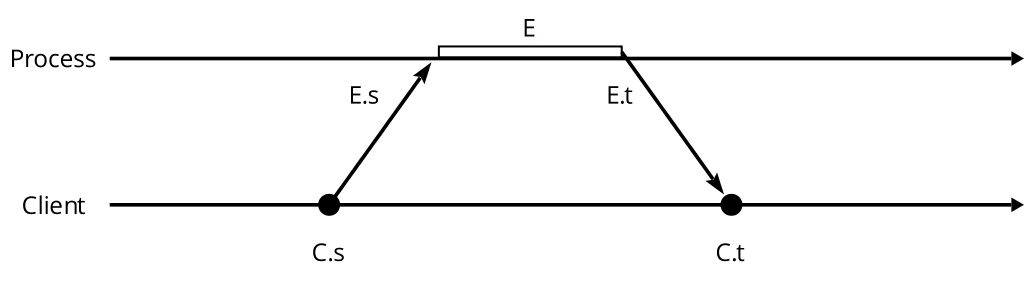
\includegraphics[scale=0.4]{images/request.png}
  \caption{Lifetime of a client request}
  \label{fig:request}
\end{figure}

While handling the request, the process may coordinate with other
processes in the background by sending and receiving more messages. For
example, the process may propagate the client's request to other
processes, retrieve up-to-date values from other processes to give to
the client, or delay handling the client's request in order to handle
other requests.

We assume clients submit two types of requests to processes. A
\emph{read request} is a request to lookup the current value of a
variable. A request to read the variable \(x\) that returns value
\(a\) is written \(R(x,a)\). A \emph{write request} is a request to
set the current value of a variable. Notation \(W(x,a)\) represents
writing value \(a\) to \(x\). We assume all processes provide access
to the same set of shared variables.

\subsubsection{Causal precedence/external order}
\label{causal-precedencehappens-beforeexternal-order}

We shall consider the full set of events across a distributed system,
such as shown in Figure \ref{fig:externalorderexec}.  This is called an
\emph{execution}. Consistency models constrain the set of allowable
return values in response to clients' requests.

\begin{figure}[h]
  \center
  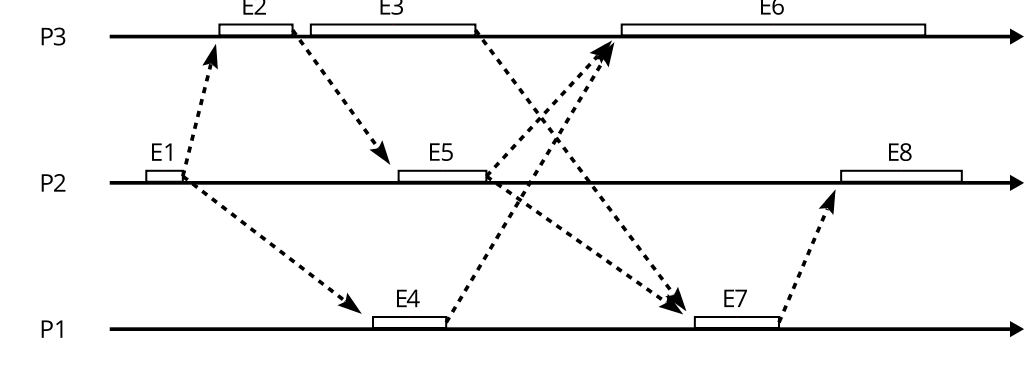
\includegraphics[scale=0.4]{images/externalorder.png}
  \caption{Depiction of external order between concurrent events across three processes. Intra-process and transitive edges are not depicted.}
  \label{fig:externalorderexec}
\end{figure}

We shall assume that requests handled by a single process do not
overlap in time. This can be enforced with local serialization methods
such as two-phase locking (CITE) that can be used to isolate
concurrent transactions from each other, providing the abstraction of
a system that handles requests one at a time. On the other hand, any
two processes may handle two events at the same physical time, so that
there is no obvious total order of events across the system. Instead,
one has a partial order called \emph{external order}.  Intuitively, it
is the partial order of events that would be witnessed by an observer
recording the real time at which systems begin and finish responding
to requests.

\begin{definition}
  Let $E$ be an execution. Request $E1$ \emph{externally precedes}
  request $E2$ if $E1.t < E2.s$. That is, if the first request
  terminates before the second request is accepted. This induces an
  irreflexive partial order called \emph{external order}.
\end{definition}

Recall that an irreflexive partial order is a binary relation \(<\) such
that \(A \not < A\), \(A < B \implies B \not < A\), and
\(A < B, B < C \implies A < C\).

Because we assume processes handle events one-at-a-time, the events
handled at any one process are totally ordered by external order---one
event cannot start before another has finished. If \(E1\) and \(E2\) are
events at \emph{different} processes, they need not be comparable by
external order, i.e.~neither \(E1.t < E2.s\) nor \(E2.t < E1.s\), making
them \emph{physically concurrent}.

\begin{definition}
  If two events overlap in physical time (equivalently, if they are
  not comparable by external order), we call the events
  \emph{physically concurrent} and write $E1 || E2$.
\end{definition}

Physical concurrency is a reflexive and symmetric---but usually not
transitive--- binary relation. Such structures are often called
\emph{compatibility relations.} The general intuition is that anything
is compatabile with itself (reflexivity), and the compatibility of two
objects does not depend on their order (symmetry). But if \(A\) and
\(B\) are compatible with \(C\), it need not be the case that \(A\)
and \(B\) are compatible with each other.

Figure \ref{fig:externalorderexec} shows the external order relation
for an execution. To save space we elide arrows between two events of
the same process and arrows that can be inferred by transitivity. This
corresponds to the directed acyclic graph structure shown in
\ref{fig:externalorderdag}.

\begin{figure}[h]
    \center
    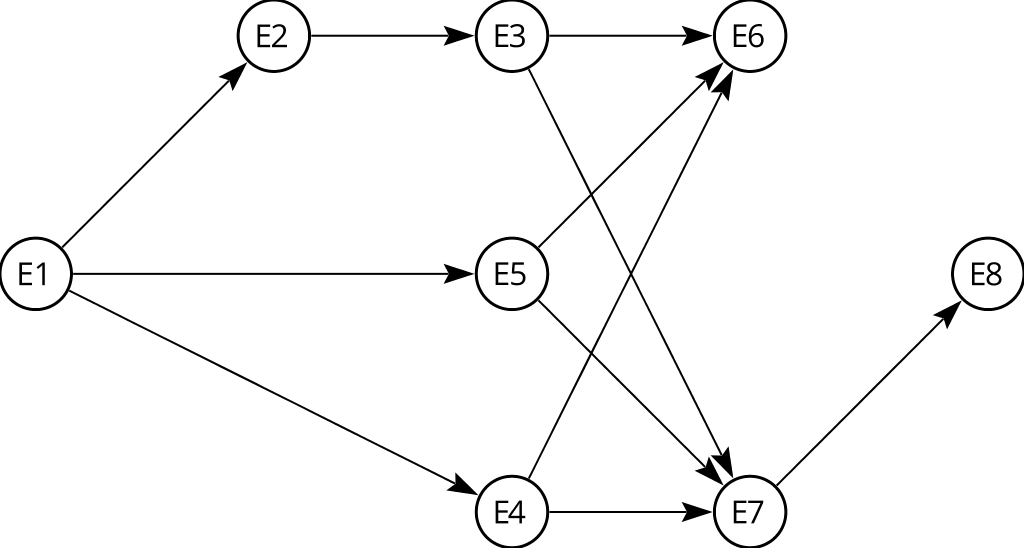
\includegraphics[scale=0.25]{images/partialorder.png}
    \caption{The directed acyclic graph (DAG) induced by external order.}
    \label{fig:externalorderdag}
\end{figure}

The reader may wonder if we can consider events to be totally ordered,
say by pairing them with a timestamp that records their physical start
time to resolve ties like \(x || y\). This order is not generally useful
for a couple reasons. First, we assume processes have only loosely
synchronized clocks, so timestamps from two different processes may not
be comparable. Additionally, even systems that enforce linearizable
consistency (c.f. Section \ref{sec:atomic}) do not necessarily handle
requests in order of their physical start times.

\subsection{Consistency Models}
\label{memory-consistency-models}

A fundamental goal for distributed computing systems is to
``{[}appear{]} to the users of the system as a single coherent
computer'' \cite{TanenbaumSteen07}. Enforcing consistency means
clients are presented with the abstraction of a shared world, as if
they are all connected to a central computer rather than than the
complex system of loosely coupled computers they are actually using.

Considering the shared memory abstraction, the requirement is that all
nodes present a \emph{mutually-consistent} view of the shared memory
to system clients. That is, as far as clients are concerned, it should
appear there is a single source of truth that all system nodes have
instantaneous access to. Bad things can happen when consistency is
violated:

\begin{itemize}
\item If two air traffic controllers were presented with conflicting
  information about the trajectory of aircraft, they could potentially
  issue dangerously incongruous instructions to pilots.
\item Messages between users that are delivered in the wrong order can
  lead to misunderstandings. For instance, it may be appear to Bob
  that Alice is responding to a different question than the one she
  meant to if her messages arrive in the wrong order.
\item A bank client would be unhappy if deposits that appear in their
  account online are not reflected when they check their balance at an
  ATM, or if they seem to disappear after refreshing the webpage.
\item Resource-dispatching systems are not useful if a resource that
  appears to be available cannot be used because the information is
  out of date. Conversely, inefficiencies result if clients think
  available resources are actually unavailable.
\end{itemize}

Strongly consistent systems are easier to understand and reason
about. Violating consistency means the abstraction of a shared
universe is broken, which can invalidate clients' mental model of the
system, make the system's behavior harder to predict, or cause safety
requirements to be violated. Clearly, all other things being equal,
one wants distributed systems to have as much consistency as
possible. However, we shall see that strong notions of consistency are
brittle in the sense that they generally cannot be achieved for the
kinds of systems we consider in this document.

What precisely constitutes consistency? A \emph{memory consistency
model} formally constrains the allowable system responses during
executions. ``Strong'' models are generally understood as ones
providing the illusion that all clients are accessing a single global
database. As we will see, this still leaves room for different
possible behaviors (i.e.~allows non-determinism in the execution of a
distributed application), but the allowable behavior is tightly
constrained.  Weaker models tolerate deviation from this standard. For
a given application, the most appropriate model depends on the
semantics expected by the application and its clients, which must be
weighed against other requirements.

\subsubsection{Linearizability/atomic consistency}
\label{sssec:linearizability}

\emph{Linearizability} (Herlihy and Wing 1990) is essentially the
strongest common consistency model. It is known variously as atomic
consistency, strict consistency, and sometimes external consistency. In
the context of database transactions (which come with other guarantees,
like isolation, that are more specific to databases), the analogous
condition is called strict serializability. A linearizable execution is
defined by three features:

\begin{itemize}
  \tightlist
\item
  All processes act like they agree on a single, global total order
  defined across all accesses.
\item
  This sequential order is consistent with the actual external order.
\item
  Responses are semantically correct, meaning a read request \(R(x, a)\)
  returns the value of the most recent write request \(W(x, a)\) to
  \(x\).
\end{itemize}

\begin{figure}\begin{subfigure}[a]{1\textwidth} \center
    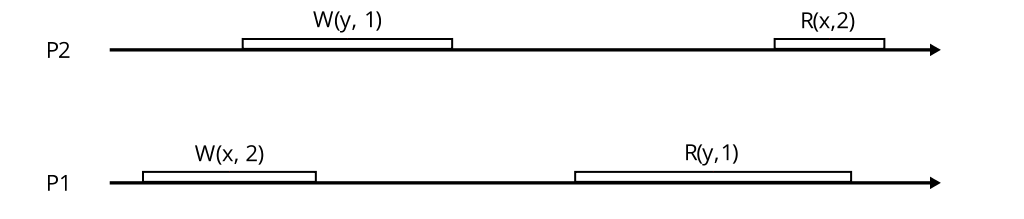
\includegraphics[scale=0.4]{images/linear1.png} \caption{A
      linearizable execution. Any choice of linearization works here.}
    \label{fig:linear_example11} \end{subfigure}
  \begin{subfigure}[b]{1\textwidth} \center
    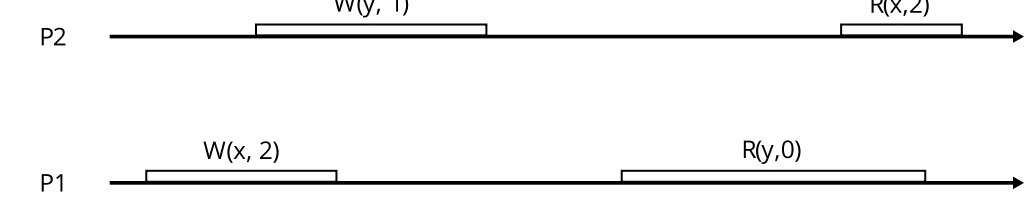
\includegraphics[scale=0.4]{images/nonlinear0.png} \caption{A
      non-linearizable execution. The request to read $y$ returns a
      stale value. } \label{fig:linear_example12} \end{subfigure}
  \caption{A linearizable and non-linearizable execution.}
  \label{fig:linear_example1} \end{figure}

Figure \ref{fig:linear_example11} shows a prototypical example of a
linearizable execution. We assume that all memory locations are
initialized to \(0\) at the system start time. Intuitively, it should
appear to an external observer that each access instantaneously took
effect at some point between its start and end time. Hence, the request
to read the value of \(y\) returns \(1\), because at some point between
\(W(y,1).s\) and \(W(y,1).t\) that change took effect. If client on
\(P_1\) read a stale value, we would say the execution is not
linearizable. Figure \ref{fig:linear_example12} shows an
non-linearizable execution that returns stale data instead of reflecting
the write access to \(y\) on \(P2\).

Linearizability can be precisely defined in terms of
\emph{linearizations.}

\begin{definition}
  A \emph{linearization point} $t \in \mathbb{R} \in [E.s, E.t]$ for an
  event $E$ is a time between the event's start and termination. An
  execution is \emph{linearizable} if and only if there is a choice of
  linearization point for each access, which induces a total order called a \emph{linearization},
  such that $E$ is equivalent to
  the serial execution of events when totally ordered by their
  linearization points.
\end{definition}

\begin{figure}[p]
  \begin{subfigure}[a]{1\textwidth}
    \center
    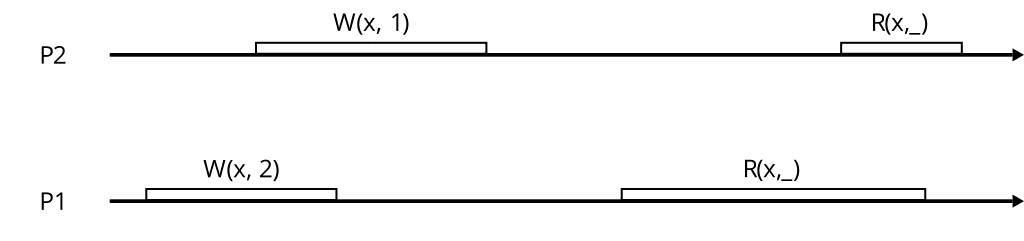
\includegraphics[scale=0.4]{images/linearTemplate.png}
    \caption{An execution with read responses left unspecified.}
    \label{fig:nonlinear}
  \end{subfigure}
  \begin{subfigure}[b]{1\textwidth}
    \center
    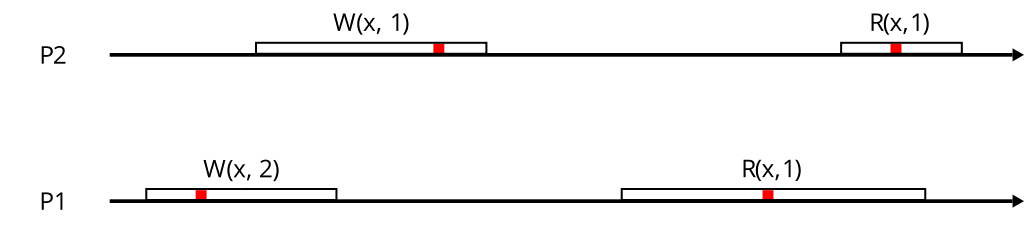
\includegraphics[scale=0.4]{images/linear3.png}
    \caption{A linearizable execution for which both reads return $1$.}
  \end{subfigure}
  \begin{subfigure}[c]{1\textwidth}
    \center
    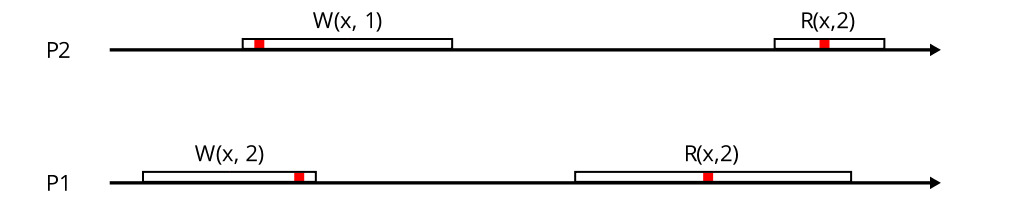
\includegraphics[scale=0.4]{images/linear2.png}
    \caption{A linearizable execution for which both reads return $2$.}
  \end{subfigure}
  \caption{Two linearizable executions of the same underlying events that return different responses. Possible linearization points are shown in red.}
  \label{fig:linearization}
\end{figure}

\begin{figure}[p]
  \begin{subfigure}[a]{1\textwidth}
    \center
    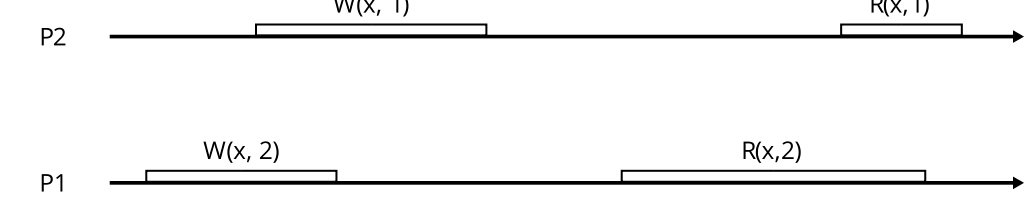
\includegraphics[scale=0.4]{images/nonlinear1.png}
    \caption{A nonlinearizable execution with the read access returning disagreeing values. We will see later (Figure \ref{fig:sequential}) that this execution is still sequentially consistent. }
    \label{fig:nonlinear1}
  \end{subfigure}
  \begin{subfigure}[b]{1\textwidth}
    \center
    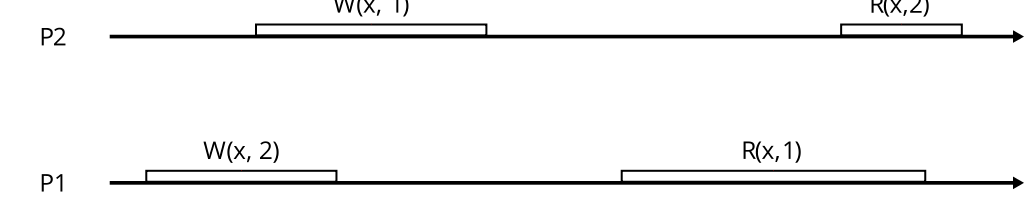
\includegraphics[scale=0.4]{images/nonlinear2.png}
    \caption{Another nonlinearizable execution with read access values swapped. This execution is not sequentially consistent.}
    \label{fig:nonlinear2}
  \end{subfigure}
  \caption{Two non-linearizable executions of the same events shown in Figure \ref{fig:linearization}.}
  \label{fig:nonlinearizable}
\end{figure}

Linearization points are demonstrated in Figure \ref{fig:linearization}.
The figure shows different linearizable behaviors in response to the
same underlying set of accesses. It is assumed no distinct access can
have the same linearization point, so that we get a total order. This
demonstrates that linearizability still leaves some room for
non-determinism in the execution of distributed applications. In this
example, the requests must both return 1 or 2. The constraint is that
the values must agree---linearizability forbids the situation in which
one client reads \(1\) and another reads \(2\) (Figure
\ref{fig:nonlinearizable}).

\begin{definition}
  We say an entire system is linearizable when all
  possible executions of the system are linearizable.
\end{definition}

\subsubsection{Sequential consistency}
\label{sequential-consistency}

Enforcing atomic consistency means that an access \(E\) at process
\(P_i\) cannot return to the client until every other process has been
informed about \(E\). For many applications this is an unacceptably high
penalty. A weaker model that is still strong enough for most purposes is
\emph{sequential} consistency. This is an appropriate model if a form of
strong consistency is required, but the system is agnostic about the
precise physical time at which events start and finish, provided they
occur in a globally agreed upon order.

A sequentially consistent system ensures that any execution is
equivalent to some global serial execution, even if this is serial order
is not the one suggested by the real-time ordering of events. When
real-time constraints are not important, this provides essentially the
same benefits as linearizability. For example, it allows programmers to
reason about concurrent executions of programs because the result is
always guaranteed to represent some possible interleaving of
instructions, never allowing instructions from one program to execute
out of order.

\begin{definition}
  \label{def:sequentiallyconsistent}
  A \emph{sequentially consistent} execution is
  characterized by three features:
  \begin{itemize}
  \item All processes act like they agree on a single, global total order
    defined across all accesses.
  \item This sequential order is consistent with the program order of each process.
  \item Responses are semantically correct, meaning reads return the most recent writes (as determined by the global order)
  \end{itemize}
\end{definition}

Processes in a sequentially consistent system are required to agree on a
total order of events, presenting the illusion of a shared database from
an application programmer's point of view. However, this order need not
be given by external order. Instead, the only requirement is that
sequential history must agree with process order, i.e.~the events from
each process must occur in the same order as in they do in the process.
This is nearly the definition of linearizability, except that external
order has been replaced with merely program order. We immediately get
the following lemma.

\begin{lemma}
  \label{lem:linearsequential}
  A linearizable execution is sequentially consistent.
\end{lemma}
\begin{proof}
  This follows because process order is a subset of external order.
\end{proof}

\begin{figure}
  \begin{subfigure}[a]{1\textwidth}
    \center
    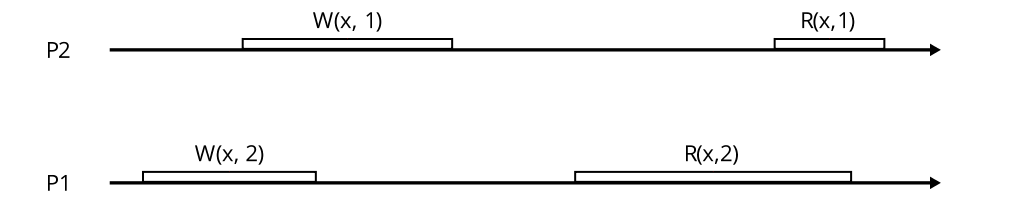
\includegraphics[scale=0.4]{images/sequential1.png}
    \caption{A non-linearizable, sequentially consistent execution.}
    \label{fig:sequential1}
  \end{subfigure}
  \begin{subfigure}[b]{1\textwidth}
    \center
    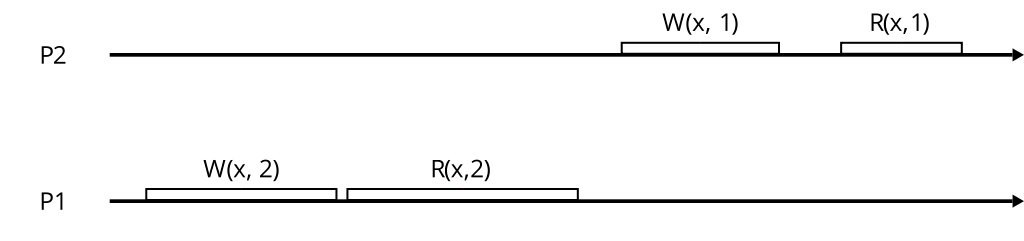
\includegraphics[scale=0.4]{images/sequential2.png}
    \caption{An equivalent interleaving of \ref{fig:sequential1}.}
    \label{fig:interleaving1}
  \end{subfigure}
  \caption{A sequentially consistent execution and a possible interleaving.}
  \label{fig:sequential}
\end{figure}

Visually, sequential consistency allows reordering an execution by
sliding events along each process' time axis like beads along a string.
Two events from the same process cannot pass over each other as this
would violate program order, but events on different processes may be
commuted past each other, violating external order. This sliding allows
defining an arbitrary interleaving of events, a totally ordered
execution with no events overlapping. From this perspective, while
linearizability requires the existence of a linearization, sequential
consistency requires the existence of an equivalent interleaving.

The converse of Lemma \ref{lem:linearsequential} does not hold. For
example, Figure \ref{fig:sequential1} was previously shown (Figure
\ref{fig:nonlinear1}) as a nonlinearizable execution. However, it is
sequentially consistent, as evidenced by the interleaving in Figure
\ref{fig:interleaving1} that slides the events \(W(x,1)\) and \(R(x,2)\)
past each other.

\begin{figure}
  \begin{subfigure}[a]{1\textwidth}
    \center
    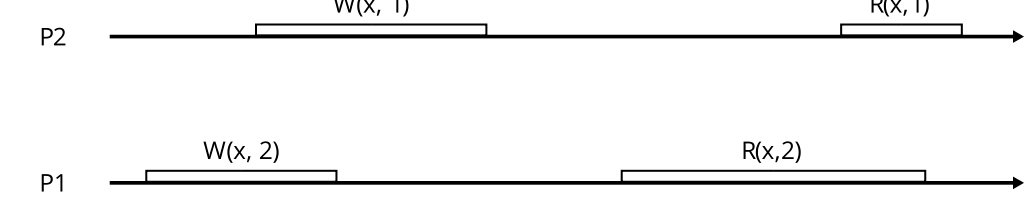
\includegraphics[scale=0.4]{images/nonsequential1.png}
    \caption{A non-sequentially consistent execution.}
    \label{fig:nonsequential1}
  \end{subfigure}
  \begin{subfigure}[b]{1\textwidth}
    \center
    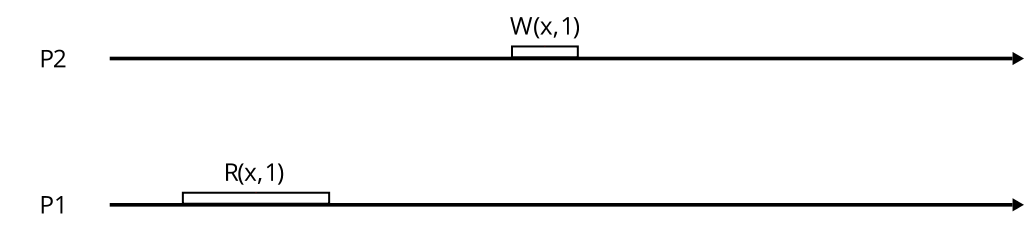
\includegraphics[scale=0.4]{images/nonsequential_x.png}
    \caption{The sequentially consistent history of $x$.}
    \label{fig:sequentialx}
  \end{subfigure}
  \begin{subfigure}[b]{1\textwidth}
    \center
    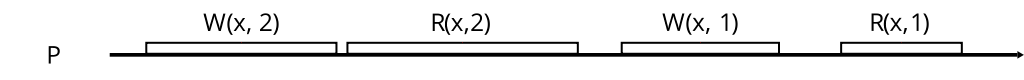
\includegraphics[scale=0.4]{images/nonsequential_y.png}
    \caption{The sequentially consistent history of $y$.}
    \label{fig:sequentialy}
  \end{subfigure}
  \caption{A non-sequentially consistent execution with sequentially-consistent executions at each variable.}
  \label{fig:nonsequential}
\end{figure}

\subsubsection{Causal consistency}
\label{causal-consistency}

\emph{Causal} consistency (CITE) is a weak (i.e. non-strong)
consistency model


\subsection{The CAP Theorem}
\label{the-cap-theorem}

Real-world systems often fall short of behaving as a single perfectly
coherent system. The root of this phenomenon is a deep and
well-understood tradeoff between system coherence and performance.
Enforcing consistency comes at the cost of additional communications,
and communications impose overheads, often unpredictable ones.

Fox and Brewer \cite{1999foxbrewer} are crediting with observing a
particular tension between the three competing goals of consistency,
availability, and partition-tolerance. This tradeoff was precisely
stated and proved in 2002 by Gilbert and Lynch
\cite{2002gilbertlynchCAP}.  The theorem is often somewhat
misunderstood, as we discuss, so it is worth clarifying the terms
used.

\paragraph{Consistency}

Gilbert and Lynch define a consistency system as one whose executions
are always linearizable.

\paragraph{Availability}

A CAP-available system is one that will definitely respond to every
client request at some point.

\paragraph{Partition tolerance}

A partition-tolerant system continues to function, and ensure whatever
guarantees it is meant to provide, in the face of arbitrary partitions
in the network (i.e., an inability for some nodes to communicate with
others). It is possible that a partition never recovers, say if a
critical communications cable is permanently severed.

A partition-tolerant CAP-available system cannot indefinitely suspend
handling a request to wait for network activity like receiving a
message. In the event of a partition that never recovers, this would
mean the process could wait indefinitely for the partition to heal,
violating availability. On the other hand, a CAP-consistent system is
not allowed to return anything but the most up-to-date value in response
to client requests. Keep in mind that any (other) process may be the
originating replica for an update. Some reflection shows that the full
set of requirements is unattainable---a partition tolerant system simply
cannot enforce both consistency and availability.

\begin{theorem}[The CAP Theorem]
  \label{thm:cap}
  In the presense of indefinite network partitions, a distributed system
  cannot guarantee both linearizability and eventual-availability.
\end{theorem}
\begin{proof}
  Technically, the proof is almost trivial. We give only the informal
  sketch here, leaving the interested reader to consult the more formal
  analysis by Gilbert and Lynch. The key technical assumption is that a
  processes' behavior can only be influenced by the messages it actually
  receives---it cannot be affected by messages that are sent to it but
  never delivered.

  In Figure \ref{fig:linear_example11}, suppose the two processes are on
  opposite sides of a network partition, so that no information can be
  exchanged between them (even indirectly through a third party). If we
  just consider the execution of $P_2$ by itself, without $P_1$,
  linearizability would require it to read the value $2$ for $y$. If we
  do consider $P_1$, linearizability requires that the read access to
  $y$ must return $1$. But if $P_2$ cannot send messages to $P_1$, then
  $P_2$'s behavior cannot be influenced by the write access to $y$, so
  it would still have to return $2$, violating
  consistency. Alternatively, it could delay returning any result until
  it is able to exchange messages with $P_1$. But if the partition never
  recovers, $P_1$ will wait forever, violating availability.
\end{proof}

\subsubsection{CAP for Sequential Consistency}

Sequential consistency is a relaxation of atomic consistency, but not by
much. The model is still too strict to enforce under partition
conditions.

\begin{lemma}[CAP for sequential consistency]
  \label{thm:cap-sequential}
  An eventually-available system cannot provide sequential consistency in the presense of network partitions.
\end{lemma}
\begin{proof}

  The proof is an adaptation of Theorem \ref{thm:cap}. Suppose $P_1$ and
  $P_2$ form of CAP-available distributed system and consider the
  following execution: $P_1$ reads $x$, then assigns $y$ the value
  $1$. $P_2$ reads $y$, then assigns $x$ the value $1$. (Note that this
  is the sequence of requests shown in Figure \ref{fig:nonsequential1},
  but we make no assumptions about the values returned by the read
  requests). By availability, we know the requests will be handled (with
  responses sent back to clients) after a finite amount of time. Now
  suppose $P_1$ and $P_2$ are separated by a partition so they cannot
  read each other's writes during this process. For contradiction,
  suppose the execution is equivalent to a sequential order.

  If $W(y,1)$ precedes $R(y)$ in the sequential order, then $R(y)$ would
  be constrained to return to $1$. But $P_2$ cannot pass information to
  $P_1$, so this is ruled out. To avoid this situation, suppose the
  sequential order places $R(y)$ before $W(y,1)$, in which case $R(y)$
  could correctly return the initial value of $0$. However, by
  transitivity the $R(x)$ event would occur after $W(x,1)$ event, so it
  would have to return $1$. But there is no way to pass this information
  from $P_1$ to $P_2$. Thus, any attempt to consistently order the
  requests would require commuting $W(y,1)$ with $R(x)$ or $W(x,1)$ with
  $R(y)$, which would violate program order.
\end{proof}


\subsubsection{Consequences of CAP}
\label{interpretation-of-the-cap-theorem}

While the proof of the CAP theorem is simple, its interpretation is
subtle and has been the subject of much discussion in the years since
\cite{2012CAP12Years}. It is sometimes assumed that the CAP theorem claims that
a distributed system can only offer two of the properties C, A, and P.
In fact, the theorem constrains, but does not prohibit the existence of,
applications that apply some relaxed amount of all three features. The
CAP theorem only rules out their combination when all three are
interpreted in a highly idealized sense.

In practice, applications can tolerate much weaker levels of consistency
than linearizability. Furthermore, network partitions are usually not as
dramatic as an indefinite communications blackout. Real conditions in
our context are likely to be chaotic, featuring many smaller disruptions
and delays and sometimes larger ones. Communications between different
clients may be affected differently, with nearby agents generally likely
to have better communication channels between them than agents that are
far apart. Finally, CAP-availability is a suprisingly weak condition.
Generally one cares about the actual time it takes to handle user
requests, but the CAP theorem exposes difficulties just ensuring the
system handles requests at all. Altogether, the extremes of C, A, and P
in the CAP theorem are not the appropriate conditions to apply to many,
perhaps most, real-world applications.

\paragraph{The safety/liveness tradeoff}

The tension between consistency and availability is a prototypical
example of a deeper tension in computing: that between safey and
liveness properties \cite{10.1145/5505.5508,2012perspectivesCAP}. These terms can be understood as follows.

\begin{itemize}
\item
  \textbf{Safety} properties ensure that a system avoids doing something
  ``bad'\,' like violating a consistency invariant. Taken to the
  extreme, one way to ensure safety is to do nothing. For instance, we
  could enforce safety by never responding to read requests in order to
  avoid offering information that is inconsistent with that of other
  nodes.
\item
  \textbf{Liveness} properties ensure that a system will eventually do
  something ``good'\,', like respond to a client. Taken to the extreme,
  one very lively behavior would be to immediately respond to user
  requests, without taking any steps to make sure this response is
  consistent with that of other nodes.
\end{itemize}

Note that ``safety'' is narrow sense, meaning a constraint on a system's
allowable responses to clients, while liveness properties require the
system to ``do'' something instead of delaying forever. Clearly, it is
important for systems in safety-related applications to have some amount
of liveness, and not just ``safety'' properties. Liveness and safety are
both good.

Because of the tension between them, building applications that provide
both safety and liveness features is challenging. The fundamental
principle is that if we want to increase how quickly a system can
respond to requests, eventually we must relax our constraints on what
the system is allowed to return.

\newpage
\section{Desiderata and assumptions}
\label{sec:desiderata}

\subsection{Assumptions}
\label{ssec:assumptions}

\begin{itemize}
\item Only very loose clock synchronization. However, we may fairly assume that nodes can measure the passage of time. Real timestamps may be collected on data (for example, for later analysis), but the correct configuration of these clocks cannot be relied upon, particularly at lower levels of abstraction.
\item
\end{itemize}

\subsection{Desiderata}
\label{ssec:desiderata}

Having discussed some of the fundamental distributed systems issues that
arise under real-world network conditions, we turn our attention to
three desiderata we will use to frame and analyze the models discussed
in Sections \ref{sec:continuous-consistency} and \ref{sec:data-fusion}.

The CAP theorem, and others like it, place fundamental limitations on
the consistency of real-world distributed systems. In the absense of a
``perfect'' system, engineers are forced to make tradeoffs. Ideally,
these tradeoffs should be tuned for the specific application in mind---a
protocol that works well in a datacenter might not work well in a
heterogeneous geodistributed setting. This section lists three desirable
features of distributed systems and frameworks for reasoning about or
implementing them. We chose this set based on the particular details of
civil aviation and disaster response, where safety is a high priority
and usage/communication patterns may be unpredictable.

\hypertarget{d1-quantifiable-bounds-on-inconsistency}{%
  \subsubsection{D1: Quantifiable bounds on
    inconsistency}\label{d1-quantifiable-bounds-on-inconsistency}}

\emph{A distributed application should quantify the amount of
consistency it delivers. That is, it should (1) provide a mathematical
way of measuring inconsistency between system nodes, and (2) bound
this value while the system is available.}

The CAP theorem implies that an available data replication application
cannot bound inconsistency in all circumstances. When bounded
inconsistency cannot be guaranteed, a system satisfying D1 may become
unavailable. Alternatively, a reasonable behavior would be to continue
providing some form of availability, but alert the user that due to
network and system use conditions the requisite level of consisteny
cannot be guaranteed by the application, leaving the user with the
choice to assess the risk and continue using the system with a weaker
safety guarantees.

\hypertarget{d2-accommodation-of-heterogeneous-nodes}{%
  \subsubsection{D2: Accommodation of heterogeneous
    nodes}\label{d2-accommodation-of-heterogeneous-nodes}}

\emph{An application should not assume that there is a typical system
node. Instead, the system should accomdate a diverse range of
heterogeneous clients presenting different capabilities, tasks, and
risk-factors.}

One can expect a variety of hardware in the field. For example,
wildfires often involve responses from many different fire departments,
and it must be assumed that they are not always using identical systems.
Different participants in the system may be solving different tasks,
with different levels of access to the network, and they present
different risks. With these sorts of factors in mind, one should hope
for frameworks that are as general as possible to accomodate a wide
variety of clients.

\hypertarget{d3-optimization-for-a-geodistributed-wide-area-network}{%
  \subsubsection{D3: Optimization for a geodistributed wide area
    network}\label{d3-optimization-for-a-geodistributed-wide-area-network}}

\emph{An application should be optimized for the sorts of
communication patterns that occur in geodistributed wide area networks
(WANs) under real-world conditions.}

Consider two incidents. Wouldn't want to enforce needless global
consistency, particularly if the agents in one area do not have the same
consistency requirements for another area.

Network throughput has some (perhaps approximately linear) relationship
with throughput. Communications patterns are likely far from uniform
too. In fact, these two things likely coincide---it is often that nodes
which are nearby have a stronger need to coordinate their actions than
nodes which are far away. For example, consider manoeauvering airplanes
to avoid crash.

\newpage

\hypertarget{resilient-network-architectures}{%
  \section{Resilient Network
    Architectures}\label{resilient-network-architectures}}

\label{sec:networking}

\hypertarget{state-of-the-art}{%
  \subsection{State of the art}\label{state-of-the-art}}

\begin{itemize}
  \tightlist
\item
  COWs and COLTs
\end{itemize}

\hypertarget{ad-hoc-networking}{%
  \subsection{Ad-hoc networking}\label{ad-hoc-networking}}

\hypertarget{physical-communications}{%
  \subsubsection{Physical communications}\label{physical-communications}}

The details of the physical communication between processes is outside
the scope of this memo. We make just a few high-level observations about
the possibilities, as the details of the network layer are likely to
have an impact on distributed applications, such as the shared memory
abstraction we discuss below and in Section
\ref{sec:continuous-consistency}. For such applications, it may be
important to optimize for the sorts of usage patterns encountered in
real scenarios, which are affected by (among other things) the low-level
details of the network.

The \emph{celluar} model (Figure \ref{fig:centralized}) assumes nodes
are within range of a powerful, centralized transmission station that
performs routing functions. Message passing takes place by transmitting
to the base station (labeled \(R\)), which routes the message to its
destination. Such a model could be supported by the ad-hoc deployment of
portable cellphone towers transported into the field, for instance.

The \emph{ad-hoc} model (Figure \ref{fig:decentralized}) assumes nodes
communicate by passing messages directly to each other. This requires
nodes to maintain information about things like routing and the
approximate location of other nodes in the system, increasing complexity
and introducing a possible source of inconsistency. However, it may be
more workable given (i) the geographic mobility of agents in our
scenarios (ii) difficult-to-access locations that prohibit setting up
communication towers (iii) the inherent need for system flexibility
during disaster scenarios.

\begin{figure}[h]
  \centering
  \begin{subfigure}[b]{0.48\textwidth}
    \centering
    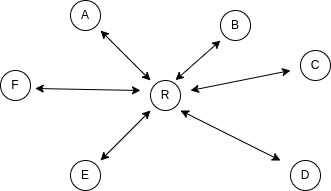
\includegraphics[width=\textwidth]{images/Centralized.png}
    \caption{Cellular network topology}
    \label{fig:centralized}
  \end{subfigure}
  \hfill
  \begin{subfigure}[b]{0.48\textwidth}
    \centering
    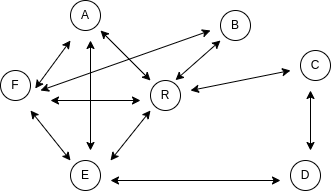
\includegraphics[width=\textwidth]{images/Decentralized.png}
    \caption{Ad-hoc network topology}
    \label{fig:decentralized}
  \end{subfigure}
  \caption{Network topology models for geodistributed agents. Edges represent communication links (bidirectional for simplicity).}
  \label{fig:nettopology}
\end{figure}

One can also imagine hybrid models, such as an ad-hoc arrangement of
localized cells. In general, one expects more centralized topologies to
be simpler for application developers to reason about, but to require
more physical infrastructure and support. On the other hand, the ad-hoc
model is more fault resistant, but more complicated to implement and
potentially offering fewer assurancess about performance. In either
case, higher-level applications such as shared memory abstractions
should be tuned for the networking environment. It would be even better
if this tuning can take place dynamically, with applications
reconfiguring manually or automatically to the particulars of the
operating environment. This requires examining the relationship between
the application and networking layers, rather than treating them as
separate blackboxes.

\hypertarget{delay-tolerant-networking}{%
  \subsection{Delay-tolerant networking}\label{delay-tolerant-networking}}

\hypertarget{ad-hoc-dtns}{%
  \subsection{Ad-hoc DTNs}\label{ad-hoc-dtns}}

An interesting possibility is for the \emph{network} to automatically
configure itself to the quality-of-service needs of the application. For
example, a client that receives a lot of requests may be marked as a
preferred client and given higher-priority access to the network. If UAV
vehicles can be used to route messages by acting as mobile transmission
base stations, one can imagine selecting a flight pattern based on
networking needs. For example, if the communication between two
firefighting teams is obstructed by a geographical feature, a UAV could
be dispatched to provide overhead communication support. Such an
arrangement could greatly blur the line between the networking and
application layers.

\hypertarget{software-defined-networking}{%
  \subsection{Software-defined
    networking}\label{software-defined-networking}}

\hypertarget{verification-of-networking-protocols}{%
  \subsection{Verification of networking
    protocols}\label{verification-of-networking-protocols}}

\newpage

\hypertarget{continuous-consistency}{%
  \section{Continuous Consistency}\label{continuous-consistency}}

\label{sec:continuous-consistency}

Strong consistency is a discrete proposition: an application provides
strong consistency or it does not. For many real-world applications, it
evidently makes sense to work with data that is consistent up to some
\(\epsilon \in \mathbb{R}^{\geq 0}\). Thus, we shift from thinking about
consistency as an all-or-nothing condition, towards consistency as a
bound on inconsistency.

The definition of \(\epsilon\) evidently requires a more or less
application-specific notion of divergence between replicas of a shared
data object. Take, say, an application for disseminating the most
up-to-date visualization of the location of a fire front. It may be
acceptable if this information appears 5 minutes out of date to a
client, but unacceptable if it is 30 minutes out of date. That is, we
could measure consistency with respect to \emph{time}. One should expect
the exact tolerance for \(\epsilon\) will be depend very much on the
client, among other things. For example, firefighters who are very close
to a fire have a lower tolerance for stale information than a central
client keeping only a birds-eye view of several fire fronts
simultaneously.

Now suppose many disaster-response agencies coordinate with to update
and propagate information about the availability of resources. A client
may want to lookup the number of vehicles of a certain type that are
available to be dispatched within a certain geographic range. We may
stipulate that the value read by a client should always be \(4\) of the
actual number, i.e.~we could measure inconsistency with respect to some
numerical value.

In the last example, the reader may wonder we should tolerate a client
to read a value that is incorrect by 4, when clearly it is better to be
incorrect by 0. Intuitively, the practical benefit of tolerating weaker
values is to tolerate a greater level of imperfection in network
communications. For example, suppose Alice and Bob are individually
authorized to dispatch vehicles from a shared pool. In the event that
they cannot share a message.

Or, would could ask that the the value is a conservative estimate,
possibly lower but not higher than the actual amount. In these examples,
we measure inconsistency in terms of a numerical value.

As a third example,

By varying \(\epsilon\), one can imagine consistency as a continuous
spectrum. In light of the CAP theorem, we should likewise expect that
applications with weaker consistency requirements (high \(\epsilon\))
should provide higher availability, all other things being equal.

Yu and Vahdat explored the CAP tradeoff from this perspective in a
series of papers \cite{2000tact,2000tactalgorithms,10.5555/1251229.1251250,DBLP:conf/icdcs/YuV01,2002tact}
propose a theory of \emph{conits}, a logical unit of data subject to
their three metrics for measuring consistency. By controlling the
threshold of acceptable inconsistency of each conit as a continuous
quantity, applications can exercise precise control the tradeoff between
consistency and performance, trading one for the other in a gradual
fashion.

They built a prototype toolkit called TACT, which allows applications to
specify precisely their desired levels of consistency for each conit. An
interesting aspect of this work is that consistency can be tuned
\emph{dynamically}. This is desirable because one does not know a priori
how much consistency or availability is acceptable.

The biggest question one must answer is the competing goals of
generality and practicality. Generality means providing a general notion
of measuring \(\epsilon\), while practicality means enforcing
consistency in a way that can exploit weakened consistency requirements
to offer better overall performance.

\begin{itemize}
\item
  The tradeoff of CAP is a continuous spectrum between linearizability
  and high-availability. More importantly, it can be tuned in real time.
\item
  TACT captures neither CAP-consistency (i.e.~neither atomic nor
  sequential consistency) nor CAP-availability (read and write requests
  may be delayed indefinitely if the system is unable to enforce
  consistency requirements because of network issues).
\end{itemize}

\hypertarget{causal-consistency-1}{%
  \subsection{Causal consistency}\label{causal-consistency-1}}

Causal consistency is that each clients is consistent with a total order
that contains the happened-before relation. It does not put a bound on
divergence between replicas. Violations of causal consistency can
present clients with deeply counterintuitive behavior.

\begin{itemize}
  \tightlist
\item
  In a group messaing application, Alice posts a message and Bob
  replies. On Charlie's device, Bob's reply appears before Alice's
  original message.
\item
  Alice sees a deposit for \$100 made to her bank account and, because
  of this, decides to withdraw \$50. When she refreshes the page, the
  deposit is gone and her account is overdrawn by \(50\). A little while
  later, she refreshes the page and the deposit reappears, but a penalty
  has been assessed for overdrawing her account.
\end{itemize}

In these scenarios, one agent takes an action \emph{in response to} an
event, but other processes observe these causally-related events taking
place in the opposite order. In the first example, Charlie is able to
observe a response to a message he does not see, which does not make
sense to him. In the second example, Alice's observation at one instance
causes her to take an action, but at a later point the cause for her
actions appears to have occurred after her response to it. Both of these
scenarios already violate atomic and sequential consistency because
those models enforce a system-wide total order of events. Happily, they
are also ruled out by causally consistent systems. The advantage of the
causal consistency model is that it rules out this behavior without
sacrificing system availability, as shown below.

Causal consistency enforces a global total order on events that are
\emph{causally related}. Here, causal relationships are estimated very
conservatively: two events are potentially causally if there is some way
that the outcome of one could have influenced another.

\begin{figure}
  \center
  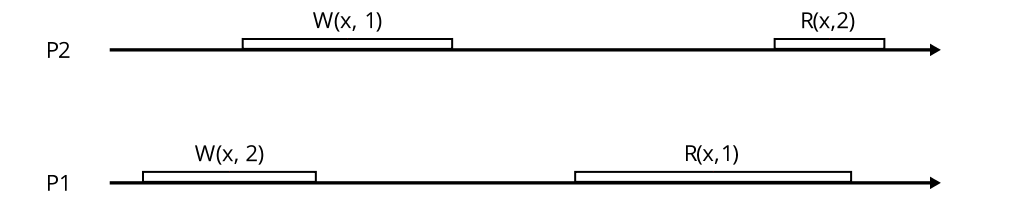
\includegraphics[scale=0.4]{images/causal1.png}
  \caption{A causally consistent, non-sequentially-consistent execution}
\end{figure}

\begin{lemma}
  Sequential consistency implies causal consistency.
\end{lemma}
\begin{proof}
  This is immediate from the definitions. Sequential consistency
  requires all processes to observe the same total order of events,
  where this total order must respect program order. Causal consistency
  only requires processes to agree on events that are potentially
  causally related. Program order is a subset of causal order, so any
  sequential executions also respects causal order.
\end{proof}

However, causal consistency is not nearly as strong as sequential
consistency, as processes do not need to agree on the order of events
with no causal relation between them. This weakness is evident in the
fact that the CAP theorem does not rule out highly available systems
that maintain causal consistency even during network partitions.

\begin{lemma}
  A causally consistent system need not be unavailabile during partitions.
\end{lemma}
\begin{proof}

  Suppose $P_1$ and $P_2$ maintain replicas of a key-value store, as
  before, and suppose they are separated by a partition. The strategy is
  simple: each process immediately handles read requests by reading from
  its local replica, and handles write requests by applying the update
  to its local replica. It is easy to see this leads to causally
  consistent histories. Intuitively, the fact that no information flows
  between the processes also means the events of each process are not
  related by causality, so causality is not violated.  \end{proof}

Note that in this scenario, a client's requests are always routed to the
same processor. If a client's requests can be routed to any node, causal
consistency cannot be maintained without losing availability. One
sometimes says that causal consistency is ``sticky available'' because
clients must stick to the same processor during partitions.

The fact that causal consistency can be maintained during partitions
suggests it is too weak. Indeed, there are no guarantees about the
difference in values for \(x\) and \(y\) across the two replicas.

\hypertarget{tact-system-model}{%
  \subsection{TACT system model}\label{tact-system-model}}

As in Section \ref{sec:background}, we assume a distributed set of
processes collaborate to maintain local replicas of a shared data object
such as a database. Processes accept read and write requests from
clients to update items, and they communicate with each other to ensure
to ensure that all replicas remain consistent.

However, access to the data store is mediated by a middleware library,
which sits between the local copy of the replica and the client. At a
high level, TACT will allow an operation to take place if it does not
violate user-specific consistency bounds. If allowing an operation to
proceed would violate consistency constraints, the operation blocks
until TACT synchronizes with one or more other remote replicas. The
operation remains blocked until TACT ensures that executing it would not
violate consistency requirements.

\[\textrm{Consistency} = \langle \textrm{Numerical error, \textrm{Order error}, \textrm{Staleness}} \rangle.\]

Processes forward accesses to TACT, which handles commiting them to the
store. TACT may not immediately process the request---instead it may
need to coordinate with other processes to enforce consistency. When
write requests are processed (i.e.~when a response is sent to the
originating client), they are only commited in a \emph{tenative} state.
Tentative writes eventually become fully committed at some point in the
future, but when they are commited, they may be reordered. After
fullying committing, writes are in a total order known to all processes.

\begin{figure}[h]
  \center
  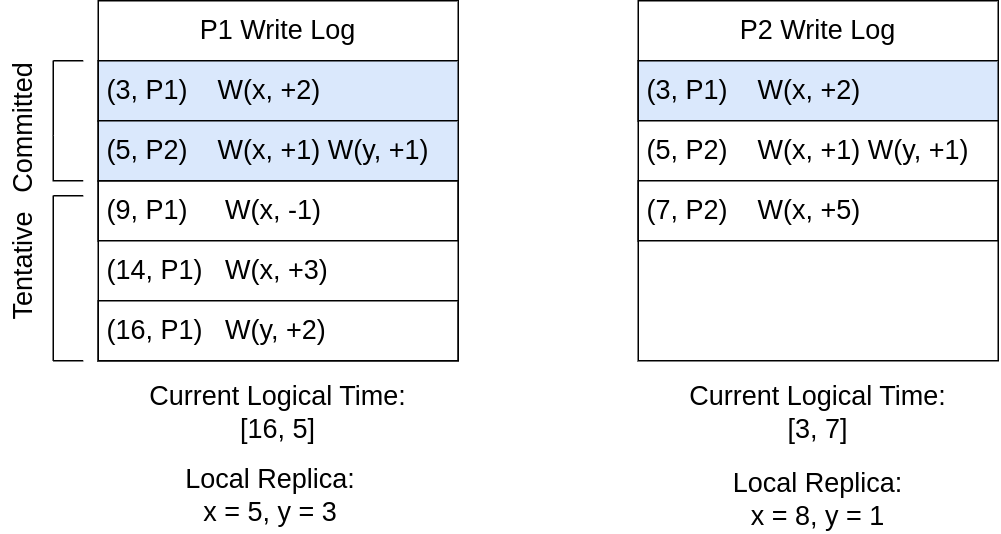
\includegraphics[scale=0.4]{images/TACT Logs.png}
  \caption{Snapshot of two local replicas using TACT}
  \label{fig:tact_logs}
\end{figure}

A write access \(W\) can separately quantify its \emph{numerical weight}
and \emph{order weight} on conit \(F\). Application programmers have
multiple forms of control:

Consistency is enforced by the application by setting bounds on the
consistency of read accesses. The TACT framework then enforces these
consistency levels.

\hypertarget{measuring-consistency-on-conits}{%
  \subsection{Measuring consistency on
    conits}\label{measuring-consistency-on-conits}}

\hypertarget{numerical-consistency}{%
  \paragraph{Numerical consistency}\label{numerical-consistency}}

\hypertarget{order-consistency}{%
  \paragraph{Order consistency}\label{order-consistency}}

When the number of tentative (uncommitted) writes is high, TACT executes
a write commitment algorithm. This is a \emph{pull-based} approach which
pulls information from other processes in order to advance \(P_i\)'s
vector clock, raising the watermark and hence allowing \(P_i\) to commit
some of its writes.

\hypertarget{real-time-consistency}{%
  \paragraph{Real time consistency}\label{real-time-consistency}}

\hypertarget{enforcing-inconsistency-bounds}{%
  \subsection{Enforcing inconsistency
    bounds}\label{enforcing-inconsistency-bounds}}

\hypertarget{numerical-consistency-1}{%
  \paragraph{Numerical consistency}\label{numerical-consistency-1}}

We describe split-weight AE. Yu and Vahdat also describe two other
schemes for bounding numerical error. One, compound AE, bounds absolute
error trading space for communication overhead. In their simulations,
they found minimal benefits to this tradeoff in general. It is possible
that for specific applications the savings are worth it. They also
consider a scheme, Relative NE, which bounds the relative error.

\hypertarget{order-consistency-1}{%
  \paragraph{Order consistency}\label{order-consistency-1}}

\hypertarget{real-time-consistency-1}{%
  \paragraph{Real time consistency}\label{real-time-consistency-1}}

\hypertarget{future-work}{%
  \subsection{Future work}\label{future-work}}

\hypertarget{data-fusion}{%
  \section{Data Fusion}\label{data-fusion}}

\cite{1999:lucien-datafusion}

\label{sec:data-fusion}

Strong consistency models provide the abstraction of an idealized global
truth. In the case of conits, the numerical, commit-order, and real-time
errors are measured with respect to an idealized global state of the
database. This state may not exist on any one replica, but it is the
state each replica would converge to if it were to see all remaining
unseen updates.

We consider distributed applications that receive data from many
different sources, such as from a sensor network (broadly defined). It
will often be the case that some sources of data should be expected to
agree with each other, but they may not. A typical scenario, we want to
integrate these data into a larger model of some kind. Essentially take
a poll, and attempt to synthesize a global picture that agrees as much
as possible with the data reported from the sensor network.

Here, we need a consistency model to measure how successful our attempts
are to synthesize a global image. And to tell us how much our sensors
agree. Ideally, we could use this system to diagnose disagreements
between sensors, identifying sensors that appear to be malfunctioning,
or to detect abberations that necessitate a response.

\hypertarget{fusion-centers}{%
  \subsection{Fusion centers}\label{fusion-centers}}

To be written.

\hypertarget{sheaf-theory}{%
  \subsection{Sheaf theory}\label{sheaf-theory}}

\hypertarget{introduction-to-presheaves}{%
  \subsubsection{Introduction to
    presheaves}\label{introduction-to-presheaves}}

\begin{definition}
  A \emph{partially order-indexed family of sets} is a family of sets indexed by a partially-ordered set,
  such that orders between the indices correspond to functions between the sets.
\end{definition}

We can also set \((P, \leq)\) \emph{acts on} the set
\(\{S_i\}_{i \in I}\).

\begin{definition}
  A \emph{semiautomaton} is a monoid paired with a set.
\end{definition}

This is also called a \emph{monoid action} on the set.

\begin{definition}
  A copresheaf is a *category acting on a family of sets*.
\end{definition}

\begin{definition}
  A presheaf is a *category acting covariantly on a family of sets*.
\end{definition}

\hypertarget{introduction-to-sheaves}{%
  \subsubsection{Introduction to sheaves}\label{introduction-to-sheaves}}

To be written.

\hypertarget{the-consistency-radius}{%
  \subsubsection{The consistency radius}\label{the-consistency-radius}}

To be written.

\hypertarget{conclusion}{%
  \section{Conclusion}\label{conclusion}}

\label{sec:conclusion}

To be written.

\section*{Bibliography}\label{bibliography}
\addcontentsline{toc}{section}{Bibliography}

\bibliographystyle{abbrv}
\bibliography{bibliography}

\end{document}
